\documentclass[twoside,AutoFakeBold=true]{ZJUthesisv2}
% 该文档中首字符为“%”的均为注释行,不会在论文中出现
% 论文默认为双面模式,需单面模式请将第一行换为如下所示:
% \documentclass[oneside]{ZJUthesis}
% \documentclass[twoside]{ZJUthesis}

% 取消目录中链接的颜色,方便打印
% 如需颜色,请将“false”改为“true”
%\usepackage{hyperref}
\hypersetup{colorlinks=false}

% 这里几行代码使得目录中的“第几章” 和后面的章节名称不致发生重叠
\makeatletter
\renewcommand{\numberline}[1]{%
\settowidth\@tempdimb{#1\hspace{0.5em}}%
\ifdim\@tempdima<\@tempdimb%
  \@tempdima=\@tempdimb%
\fi%
\hb@xt@\@tempdima{\@cftbsnum #1\@cftasnum\hfil}\@cftasnumb}
\makeatother

\usepackage{enumitem}
% \usepackage[linesnumbered,ruled,vlined]{algorithm2e}
\usepackage{caption}
\usepackage{algorithm}
\usepackage{algorithmicx}
\usepackage{algpseudocode}
\renewcommand{\algorithmicrequire}{\textbf{Input:}}  
\renewcommand{\algorithmicensure}{\textbf{Output:}}  

\usepackage{listings} 
\usepackage{xcolor}
\lstset{numbers=left,numberstyle=\tiny,keywordstyle=\color{blue!70},commentstyle=\color{red!50!green!50!blue!50},frame=shadowbox, rulesepcolor=\color{red!20!green!20!blue!20},escapeinside=``,xleftmargin=2em,xrightmargin=2em, aboveskip=1em}

\usepackage{makecell}

\begin{document}
%%%%%%%%%%%%%%%%%%%%%%%%%%%%%
%% 正文字体设定
%%%%%%%%%%%%%%%%%%%%%%%%%%%%%
% \songti
\fangsong


%%%%%%%%%%%%%%%%%%%%%%%%%%%%%
%% 论文封面部分
%%%%%%%%%%%%%%%%%%%%%%%%%%%%%
% 中文封面内容

% 中图分类号
\classification{TP242.6}

% 单位代码
\serialnumber{10335}

% 密级,如需密级则将其前“%”去掉
\SecretLevel{无}

% 学号
\PersonalID{21532112}
% \PersonalID{}

\title{采用随机蕨回归的工业零件六维姿态估计}
% 如果标题一行写不下,就写成两行,在下面的命令里写第二行,不需要两行则注释掉
% \titletl{物体六维位姿估计与检测}
% \titletl{test}

%英文题目
\Etitle{6D Pose Estimation of Industrial Parts }
% 如果一行写不下,同中文题目设定,一行写不下则写两行,不需要就注释掉
\Etitletl{Based on Random Ferns Regression}

% 作者
\author{陈乙宽}
% \author{}

\degree{硕士}

% 导师
\supervisor{熊\quad 蓉\quad 教\quad 授}
% \supervisor{}

% 合作导师,如果有的话,去掉注释,
%\cpsupervisor{某 \quad某某}

% 专业名称
\major{控制科学与工程}

% 研究方向
\researchdm{机器人}

% 所属学院
\institute{控制科学与工程学院}

%论文提交日期
\submitdate{2018年1月10日}

% 答辨日期
\defenddate{2018年3月10日}
\defenddateE{March 10th, 2018}

% 生成封面
\makeCoverPage

%---------------------------以下匿名-----------------------

%%%%%%%%%%%%%%%%%%%%%%%%%%%%%%
%% 中文题名页内容
%%%%%%%%%%%%%%%%%%%%%%%%%%%%%%
% 论文评阅人信息 注意两字名与三字名,两字职称与三字职称的写法,便于对齐
% 多余的名额直接注释掉即可,比如三个评阅人,把评阅人D,E注释掉即可
% \reviewersA{丘处机\hspace{1.5em}真人\hspace{1.5em}登州滨都宫\hspace{1em}}
% \reviewersB{葛\quad 洪\hspace{1.5em}方士\hspace{1.5em}罗浮山道观\hspace{1em}}
% \reviewersC{寇谦之\hspace{1.5em}天师\hspace{1.5em}嵩山中岳道场}
% \reviewersD{张三丰\hspace{1.5em}真君\hspace{1.5em}武当玉虚宫\hspace{1em}}
% \reviewersE{孙玄清\hspace{1.5em}真人\hspace{1.5em}崂山明霞洞\hspace{1em}}
\reviewersA{杨马英\hspace{1.5em}教授\hspace{1.5em}浙江工业大学\hspace{1em}}
\reviewersB{匿\quad 名}
\reviewersC{匿\quad 名}
\reviewersD{匿\quad 名}
\reviewersE{}

% 答辩委员会信息,如果某一个单位比较长,
% 请在其它较短后面补上{hspace{Xem}},X是比最长的单位名少几个字
% 如果实际人数少于6人,多余的注释掉即可
% \chairman{唐三藏\hspace{1.5em}功佛\hspace{1.5em}洛阳大慈恩寺}
% \commissionerA{惠\quad 能\hspace{1.5em}方丈\hspace{1.5em}曹溪宝林寺\hspace{1em}}
% \commissionerB{智\quad 顗\hspace{1.5em}方丈\hspace{1.5em}天台山国清寺}
% \commissionerC{法\quad 藏\quad 大和尚\quad 洛阳佛授记寺}
% \commissionerD{道\quad 济\hspace{1.5em}和尚\hspace{1.5em}临安灵隐寺\hspace{1em}}
% \commissionerE{降\quad 龙\hspace{1.5em}尊者\hspace{1.5em}天竺大雷音寺}
\chairman{}
\commissionerA{}
\commissionerB{}
\commissionerC{}
\commissionerD{}
\commissionerE{}

% 生成中文题名页
\maketitle


%%%%%%%%%%%%%%%%%%%%%%%%%%%%%%
%% 英文封面内容,硕士论文可不要此页
%%%%%%%%%%%%%%%%%%%%%%%%%%%%%%
% %英文题目
% \Etitle{6D Pose Estimation and Detecting of Objects for}
% % 如果一行写不下,同中文题目设定,一行写不下则写两行,不需要就注释掉
% \Etitletl{Industrial Programming by Demonstration}
%英文题目
\englishtitle{6D Pose Estimation and Detecting of Objects for}
% 如果一行写不下,同中文题目设定,一行写不下则写两行,不需要就注释掉
\englishtitletl{Industrial Pipeline}
% % 英文题名
% \englishtitle{HVlab~\LaTeX~Fast Guide}
% % 如果题名一行写不下,就写到第二行,不需要则将其注释掉
% \englishtitletl{The Second Edition}

% 评阅人信息,名字,职称,单位尽量用简写,否则会写不下
% \EreviewersA{Name\hspace{1.5em}Professional Title\hspace{1.5em}Organization}
% \EreviewersB{Name\hspace{1.5em}Professional Title\hspace{1.5em}Organization}
% \EreviewersC{Name\hspace{1.5em}Professional Title\hspace{1.5em}Organization}
% \EreviewersD{Name\hspace{1.5em}Professional Title\hspace{1.5em}Organization}
% \EreviewersE{Name\hspace{1.5em}Professional Title\hspace{1.5em}Organization}
\EreviewersA{Maying Yang\hspace{1.5em}Professor\hspace{1.5em}ZJUT}
\EreviewersB{Anonymous}
\EreviewersC{Anonymous}
\EreviewersD{Anonymous}
\EreviewersE{}

% 答辩委员会信息,同样尽量用简写,否则会写不下
% \Echairman{Name\hspace{1.5em}Professional Title\hspace{1.5em}Organization}
% \EcommissionerA{Name\hspace{1.5em}Professional Title\hspace{1.5em}Organization}
% \EcommissionerB{Name\hspace{1.5em}Professional Title\hspace{1.5em}Organization}
% \EcommissionerC{Name\hspace{1.5em}Professional Title\hspace{1.5em}Organization}
% \EcommissionerD{Name\hspace{1.5em}Professional Title\hspace{1.5em}Organization}
% \EcommissionerE{Name\hspace{1.5em}Professional Title\hspace{1.5em}Organization}
\Echairman{}
\EcommissionerA{}
\EcommissionerB{}
\EcommissionerC{}
\EcommissionerD{}
\EcommissionerE{}

% 生成英文封面
\makeenglishtitle


%%%%%%%%%%%%%%%%%%%%%%%%%%%%%%
%% 原创声明与版权协议页
%%%%%%%%%%%%%%%%%%%%%%%%%%%%%%

\SignautreDateA{}{}{}
\SignautreDateB{}{}{}
\SignautreDateC{}{}{}
% 生成原创声明与版权协议页
\makeOSandCPRTpage

% ---------------------------以上匿名-----------------------

%%%%%%%%%%%%%%%%%%%%%%%%%%%%%%
%% 论文部分开始
%%%%%%%%%%%%%%%%%%%%%%%%%%%%%%
\ZJUfrontmatter

%%%%%%%%%%%%%%%%%%%%%%%%%%%%%%
%% 勘误页,一般没有
%%%%%%%%%%%%%%%%%%%%%%%%%%%%%%
%\begin{corrigenda}
这是一个勘误\index{勘误}章节,一般情况下是没有的。
\end{corrigenda}


%%%%%%%%%%%%%%%%%%%%%%%%%%%%%%
%% 致谢页
%%%%%%%%%%%%%%%%%%%%%%%%%%%%%%
% \begin{thanks}
在我写这个文档的过程中,得到了网络上很多网贴的帮助,在此感谢baidu,Google,感谢
~CTeX 社区http://www.ctex.org,\LaTeX{}学习园地:http://blog.sina.com.cn/wangzhaoli11,
中科大~CTAN~镜像http://mirrors.ustc.edu.cn/CTAN/,水木社区\TeX{}版等网站、论坛,
其他一些较小的个人网站,论坛不再一一点名,在此一并感谢。
感谢浙江大学数学系提供的原始模版,感谢88\TeX{}版。
\end{thanks}

\begin{thanks}
时间飞逝,转眼就在浙江大学控制科学与工程学院机器人实验室度过了两年半时间里,我将永远不会忘记来自导师、同学、 朋友和家人的指导、帮助、关心和理解。你们的支持是我一直以来的安心科研的动力。
在此期间首先要衷心感谢我的导师,熊蓉教授。

从本科大一就开始着迷于机器人小制作的我,通过熊老师带头组织的“中控杯”机器人竞赛更深刻地体会到了机器人能给我带来的快乐。我也因此走上了研究机器人领域的求学之路,并在本科期间就得到了熊老师细心的指导和点拨。进入研究生后,熊老师依旧不遗余力地给我们传授经验和知识,同时给我以及整个实验室同学提供了绝对丰富的科研平台,让我能够顺利地进行各种实验。除此之外,熊老师总是能够在我科研遇到瓶颈的时候给我带来如母亲般地关怀,并且能给出非常好的建议和启发,带我从低谷中爬出。不光在科研上我能够在熊老师的指导下快速成长,每周一次的组会熊老师必定亲自指导我们如何展示自己的科研工作,如何清晰地表达自己的想法和成果。以及在文献撰写中,每一次都能得到熊老师细心的点评,让我从中学到了严谨的治学态度。生活中,熊老师也特别和蔼可亲,能够在团建活动中给我们带来食堂里吃不到的美味佳肴,还常常在出差途中不忘给我们捎带当地特色的礼物,分外感动。机器人实验室大家庭里,熊老师一直都是我们的姐姐,在实验室里的生活也将成为我一生中珍贵的记忆。

其次,也要感谢浙江大学机器人实验室里与我朝夕相处的每一位同学,你们的陪伴和帮助给了我前进 的动力。尤其感谢方立师兄、誉洪生师兄、王亚彪师兄、王鹏师兄、胡晋师兄、王军南师兄以及赵永生师兄在平时学术上给予的大力指导,从你们身上我学到的东西甚至超过了平时上课所学的内容。同时也要感谢王文、陈颖、李东轩、唐立、王浩、吴珺等和我一起进入实验室的挚友们,与你们相处的过程中我受益颇深。我将永远不会忘记与你们在一起的时光。

最后,感谢父母的养育之恩,也是你们一步一步的引导和教育才能让我慢慢走到今天。感谢周围所有理解我支持我的同学和益友,是你们的陪伴让我的生活充满阳光。

\end{thanks}


%%%%%%%%%%%%%%%%%%%%%%%%%%%%%%
%% 序言页
%%%%%%%%%%%%%%%%%%%%%%%%%%%%%%
% \begin{preface}
	
一晃又是快两年过去了,在使用中,我又对这个模版的部分内容进行了一定的微调,主要体现在:目录默认为分层结构,不再是以前默认是都顶格的结构;对脚注与正文的距离进行了调整,避免出现以前版本中的脚注离底部距离过大的问题;增加了对子图的支持;修正了第四级标题的字体等。整体上与上一版的没有大的区别,只有一些外观上的优化。这一版也基本是这个模版的最终稿了。接下来的部分仍然是以前的序言,仍然跟在下面。
	
上一版发布于2011年10月26日,发布之后的近两年来,陆陆续续收到一些邮件问关于使用中的一些问题,
我也算基本上做到一一解答。
同进也在着手准备根据提到的问题对这一版模版进行一定的修订,增补一些使用中普遍关心的难点问题。
因为事务冗杂缠身,加上关于参考文献格式调整部分的内容一直没有时间看明白,这个事情就一直拖下来了。
直到前一段断断续续看完了参考文献格式整理部分的帮助资料,搞清楚了它的实现思路原理,
才算又着手修订这一版教程。

在这过去的一年多里,接触到了\XeTeX{},对其强大的直接调用系统字体的能力表示赞叹,
于是将这个模版切换到了\XeTeX{}的环境下,将文件代码换成了对多语言兼容更好的UTF-8代码,
但同时保留对GBK码的兼容,具体不同之处会在后面的章节中提到。
因此新的一版分为UTF-8和GBK两个版本进行发布,两个版本使用上只有很细微的区别,
一般使用过程中可以忽略这个差别。

以下是原来的序言,此处照旧附上。


很早就听说过\LaTeX\index{\LaTeX}了,但却一直没有真正学习过,直到今年,需要处理一些大文档,想起了\LaTeX{}。
重新翻出\LaTeX{}的文档,从CCT开始,至于为什么是CCT,
因为Ctex\index{CTeX}提供的那个CTeX FAQ里对中文的第一个例子,就是以CCT
为例写的。
CCT是中科院的张林波研究员写的,帮助文档都是中文,看起来比较容易,但毕竟是好几年前的版本了,
更新也并不是那么及时,而且CCT\index{CCT}早期版本的字体是点阵字体,边缘很粗糙,
虽然不影响打印,但在这个年代还在用着这样的字体,着实不是那么舒服。
我又开始了第二个例子,CJK的尝试,在尝试CJK\index{CJK}的过程中,
无意中看到了CTeX的ctexart,ctexbook和ctexrep这几个基本模版,这才找到CTeX的门,
筒子们不要笑我绕了这么一大圈才摸进了CTeX的门,虽然从开始就使用的是CTeX的发行版。

这里也要说一下,CTeX提供的部分帮助文档内容也比较老了,一些操作现在新的软件虽然仍然兼容,
但已经不是新版软件推荐的做法了,比如,CTeX FAQ里面对于pdf文件的生成,
依然是先由latex.exe生成dvi文件,再由dvi文件生成ps文件,最后再生成pdf文件。
实际上,现在流行的新版\TeX{}类软件都已经将pdfTeX\index{pdfTeX}作为默认引擎,支持直接生成pdf文件,
而且dvi、ps文件的打开速度比pdf反而要慢许多。我使用的是64位系统,CTeX提供的安装包只支持32位系统,
我单独安装的MikTeX\index{MikTeX} x64\index{x64}版使用CTeX模版生成的dvi文件使用dvips\index{dvips}处理时会找不到字体,
因为这个问题,我找了很久,最后的结论是:dvips可以放弃了,直接使用dvipdfm\index{dvipdfm}更合适。

后来几天在\LaTeX{}的实践中看不少相关细节,开始对其模版产生了兴趣,
在88上\TeX{}版把置顶的ZJUthesis下了下来,就是写这个模版的基础,数学系模版。
下下来后发现这个模板给的例子pdf与当前学校使用的2008年论文模版差别老大了,从封面到目录,
章节格式,都是完全不一样,因此,决定着手做一个与学样提供的Word模版比较接近的模版。

在以2006年数学系模版为基础进行新模版编写的过程中,学了不少方法,
也发现老模版不少过时或者不合适的地方。
第一个学到的就是,从模版一开头就发现这个模版是以ctexbook这个模版为基础制作的,
做到模版完成的时候,
发现88的\TeX{}版置顶模版已经更新,我以为我白做了,
下下来一看,原来这个新的模版不是以ctexbook为基础制作的,而是更基础的\LaTeXe\index{\LaTeX}
对比自己基本完工的模版,才发现ctexbook为我省了很多工作量。只是一些修修改改就做到了很接近学校
word模版的效果。
ctexbook的新版已经直接将hyperref包打了进去,2006年数学系模版对hyperref\index{hyperref}的引用判断部分已经明显示过时,在用新版MikTeX运行的时候直接报错了。
在编写封面的时候,发现2006年的模版用了一个五列的表格,可这部分的内容只需要两列就够了,
直到我某天下载了中科院的模版后才明白,2006年版模版是从中科院模版改编而来,
中科院模版在封面上名字等内容的排列方式需要采用五列表格。这一部分,我也将其重新编写。

随着时代的推进,\LaTeX{}的各种功能包日渐丰富,很多过去只能从\LaTeXe{}代码写的功能,
如今可以通过相应的功能包直接实现,在这个模版中,我使用了几个新的功能包,
其中最新的当属刚刚发布的hyperref更新包,增加了hidelinks命令,可以直接将链接的边框去掉,
不用采用将边框颜色设为白色的方式了。

就像\LaTeX{}的版本总是在接近$\pi$的值一样,这份模版并不是完美的,比如对数学系的定理体系支持不足,
留在以后版本再发布或者请有兴趣的爱好者共同修改。编写这一版本的基本目的是没有任何\LaTeX{}基础的同学可以比较轻松地利用它给自己的毕业论文排一个满意的版面,整个模版没有留太多选项,
可供修改的选项只有两个:单面双面的选择和链接的颜色的有无。在模版中,我对绝大多数的语句,
都做了中文注释,解释其作用,方便有兴趣的同学研究,我也是一个初学者,作出的这份模版,
我想,应该是比较适合初学者胃口的。

\end{preface}


%%%%%%%%%%%%%%%%%%%%%%%%%%%%%%
%% 摘要
%%%%%%%%%%%%%%%%%%%%%%%%%%%%%%
\begin{abstract}
% 随着工业机器人应用领域的不断发展,简化机器人编程、降低对专业人才依赖、加快编程速度成为一个重要发展需求,也成为工业机器人领域的重要研究课题之一。演示编程提供了一种新的向机器人传递信息的方式,是简化机器人编程的重要途径。与传统机器人编程方法相比,它可以大大降低行业应用技术人员在机器人使用和编程方面所需的专业性知识要求,对于机器人的推广应用具有重要意义。物体的六维位姿估计是演示编程技术中一个非常重要的环节。通过自动化的视觉系统对工业零件进行位姿估计,可以简化机器人编程中对机器人操作点位的部署过程,从而提高工业生产的效率。但目前没有一套较为实用的物体位姿估计算法,因此本文提出了一套简单易用的物体六维位姿估计算法框架,其核心思想对于演示编程技术的发展具有一定促进意义。本文主要研究内容与成果如下:
随着工业机器人应用领域的不断发展,物体的六维位姿估计是成为当下进一步提高自动化水平的一个重要研究内容。通过自动化的视觉系统对工业零件进行位姿估计,可以简化对机器人操作点位的部署过程,大大解放人力,从而提高工业生产的效率。本文面向目前柔性制造领域中工业零部件存在姿态随机、存在局部遮挡等问题提出了一套简单易用的物体六维位姿估计算法框架,其核心思想是通过仿真环境借助级联回归框架来构建物体位姿估计模型。本文主要研究内容与成果如下:

\begin{itemize}
\item 归纳整理了随机蕨算法应用于回归问题的解决方案,并提出了一种面向大噪声干扰增加掩码机制的改进随机蕨回归算法。随机蕨算法在研究初期被用于解决分类问题,具有比随机森林算法更为优秀的精度以及效率,但缺点在于不能应用于回归问题。本文通过总结前人经验,给出了随机蕨算法应用于回归问题的解决方案。并针对实际问题中很多特征输入存在较大干扰的情况,提出了一套改进的随机蕨算法。经过本文改进后的随机蕨算法可以利用较易获取的特征置信度掩码进行有选择作出修正,使得随机蕨算法在遇到局部大噪声干扰的情况下仍然可以保持较好的回归精准度,提升了鲁棒性。

\item 搭建了一套深度相机仿真环境平台,通过借助OpenGL工具,能够实现在短时间内给出大量带有真值标注的仿真深度图像数据。这些仿真数据可以用于训练对应工业零件的位姿估计模型,从而为物体位姿估计算法开发提供了高效方便的基础环境。该仿真环境能够预先加载工业现场的深度背景信息,同时也可以模拟复杂环境下物体被随机遮挡的情况,使得最后得到的仿真深度图像更为真实以及丰富,从而让位姿估计模型的训练结果与真实数据训练出的模型更为接近。最后还提出了如何对真实深度相机采集到的深度图像中的空洞进行修补的办法,进一步缩小了仿真深度图像与真实深度图像之间差别。

\item 提出了一种像素差特征的图像特征描述方法和采用改进随机蕨回归的物体六维位姿估计算法。首先提出了一种基于深度图像中的像素差特征的全新深度图像特征描述方法。该特征描述方法具有非常高的计算效率,同时具有尺度不变性,能够很好捕捉深度图像中指定位置的物体位姿信息。然后采用有监督学习的特征哈希表达方法,显著提高原始特征的信噪比,使得物体位姿估计模型的训练更加鲁棒。随后借助本文提出的随机蕨回归算法,提出了一套针对物体位姿估计的级联回归算法框架,修正了普通级联回归算法框架中回归目标过于固定的不足。最后还利用改进后的随机蕨回归算法,提出了一种遮挡情况下物体位姿估计算法,以及利用位姿回归所用的特征描述进行物体检测,形成一套完整的从物体定位到物体位姿估计算法框架。
\end{itemize}


\keywords{位姿估计,随机蕨,仿真深度相机,物体检测}
\end{abstract}


%%%%%%%%%%%%%%%%%%%%%%%%%%%%%%
%% 英文摘要
%%%%%%%%%%%%%%%%%%%%%%%%%%%%%%
\begin{englishabstract}
The quick brown fox jump over the lazy dog.

\TeX\index{\TeX}

\englishkeywords{\TeX}

\end{englishabstract}


%%%%%%%%%%%%%%%%%%%%%%%%%%%%%%
%% 插图列表
%%%%%%%%%%%%%%%%%%%%%%%%%%%%%%
% \ZJUListofFigures

%%%%%%%%%%%%%%%%%%%%%%%%%%%%%%
%% 表格列表
%%%%%%%%%%%%%%%%%%%%%%%%%%%%%%
% \ZJUListofTables

%%%%%%%%%%%%%%%%%%%%%%%%%%%%%%
%% 缩写、符号清单、术语表
%%%%%%%%%%%%%%%%%%%%%%%%%%%%%%
% \begin{ListofSymbol}
缩写、符号清单、术语表
\end{ListofSymbol}


%%%%%%%%%%%%%%%%%%%%%%%%%%%%%%
%% 目录页
%%%%%%%%%%%%%%%%%%%%%%%%%%%%%%
\ZJUcontents



%%%%%%%%%%%%%%%%%%%%%%%%%%%%%%
%% 正文内容部分开始
%%%%%%%%%%%%%%%%%%%%%%%%%%%%%%
\ZJUmainmatter

\chapter{绪论}

\section{研究背景}

近年来,具有高效率和高精度优势的工业机器人不断解放人力加速生产,在零件制造业电子产品制造业等工业场景中都发挥着巨大的作用。同时伴随着例如3C、五金、家具等各个离散制造行业的迅速发展,同时这些行业制造普遍具有典型的柔性制造特性,也就是多品种、小批量、短周期,它们的生产节奏和产品迭代频率都相当快。这就给工业机器人部署的快速性、便捷性都提出了非常高的要求。而传统工业机器人的编程模式越来越难以适应这种要求。因此,提高工业机器人的易用性(Ease of Use),特别是简化装配作业编程(Ease of Programming),已经成为工业机器人自动化领域亟需解决的一个问题。

\begin{figure}[htb]
	\subfigure[机械臂非映射式示教]{ 
		\begin{minipage}[b]{0.5\textwidth} 
		\centering
		% \label{fig:SubFigure1} %% label for second subfigure 
		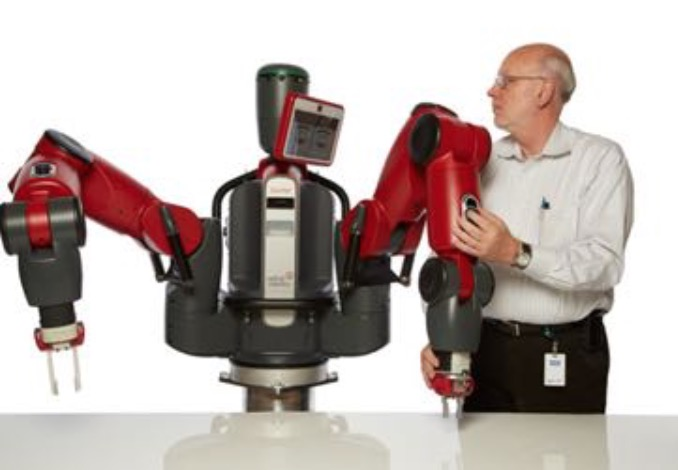
\includegraphics[scale=0.3]{./mypic/机器人示教非映射式.jpg} 
		\end{minipage}}
	\subfigure[机械臂映射式示教]{ 
		\begin{minipage}[b]{0.5\textwidth} 
		\centering
		% \label{fig:SubFigure1} %% label for second subfigure 
		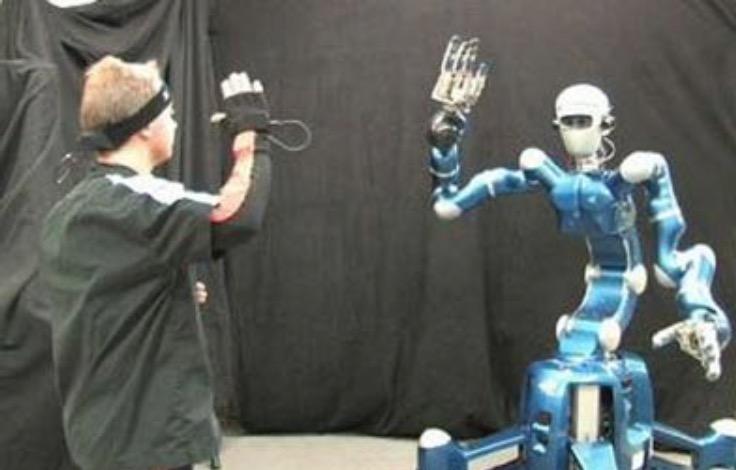
\includegraphics[scale=0.3]{./mypic/机器人示教映射式.jpg} 
		\end{minipage}}
	\caption{两种经典的演示编程示教方式}
\end{figure}

演示编程(Programming by Demonstration, 简称PbD)是目前工业研究一个非常前沿的话题,能够通过非常简单的操作方式降低工业机器人的操作复杂度。演示编程,也称为演示学习(Learning from Demonstation, 简称LfD),是由机器人系统从人的操作演示中提取理解有效信息,进而将该信息转化为机器人的程序和运动以及操作参数,从而使机器人完成相应的操作\cite{billard2008robot}。演示编程提供了一种新的向机器人传递信息的方式,是简化机器人编程的重要途径\cite{argall2009survey}。与传统机器人编程方法相比,它可以大大降低行业应用技术人员在机器人使用和编程方面所需的专业性知识要求,对于机器人的推广应用具有重要意义。但演示编程对机器人系统的智能性,特别是如何从人的操作演示中提取理解有效信息、并将该信息转化为可完成所要求作业任务的机器人程序,提出了巨大挑战。演示编程研究从上个世纪80年代中期开始,经过长期的研究,已经在运动轨迹学习领域取得了较为丰硕的成果,包括示教人演示动作的数据采集、映射和模型学习与泛化应用。上图为两种经典的演示编程示教方式。

对零件或者通用物体的位姿估计是众多演示编程示教任务中的一个基本核心任务。例如下图工业环节所示,需要将一些零件从传送带或者Tray盘上抓去抓取进行装配,或者放置到下一个工业环节中去,这其中就须要工业机器人知晓零件的位姿。通常传统方法是通过将零件整齐有规律地放置在一些有卡位结构的传送带或者Tray盘中,使得零件相对于工业机器人的位姿是绝对固定的。用这样的方法的确能直接解决问题,但同时也带来了例如机械臂标定,Tray盘传送带标定等一系列附加问题。并且这些标定问题通常是非常繁琐,非常浪费人力物力的。再加上目前由于工业场景是多变和复杂的,特别是柔性制造领域,工业零件也随着需求的变化而日新月异,一旦零件规格发生变化或是工艺发生了更新,所有的生产就会立马收到限制,极大降低了工业生产效率。但如果有一套高效便捷的零件位姿估计系统,就完全可以解决上述所有问题,大大降低生产空档时间,提升产出效率。因此对零件的位姿估计的研究具有非常高的工业应用价值和学术研究价值。因此本文将针对零件位姿估计展开研究。

\begin{figure}[htb]
	\subfigure[工业机器人抓取Tray盘上的零件]{ 
		\begin{minipage}[b]{0.5\textwidth} 
		\centering
		% \label{fig:SubFigure1} %% label for second subfigure 
		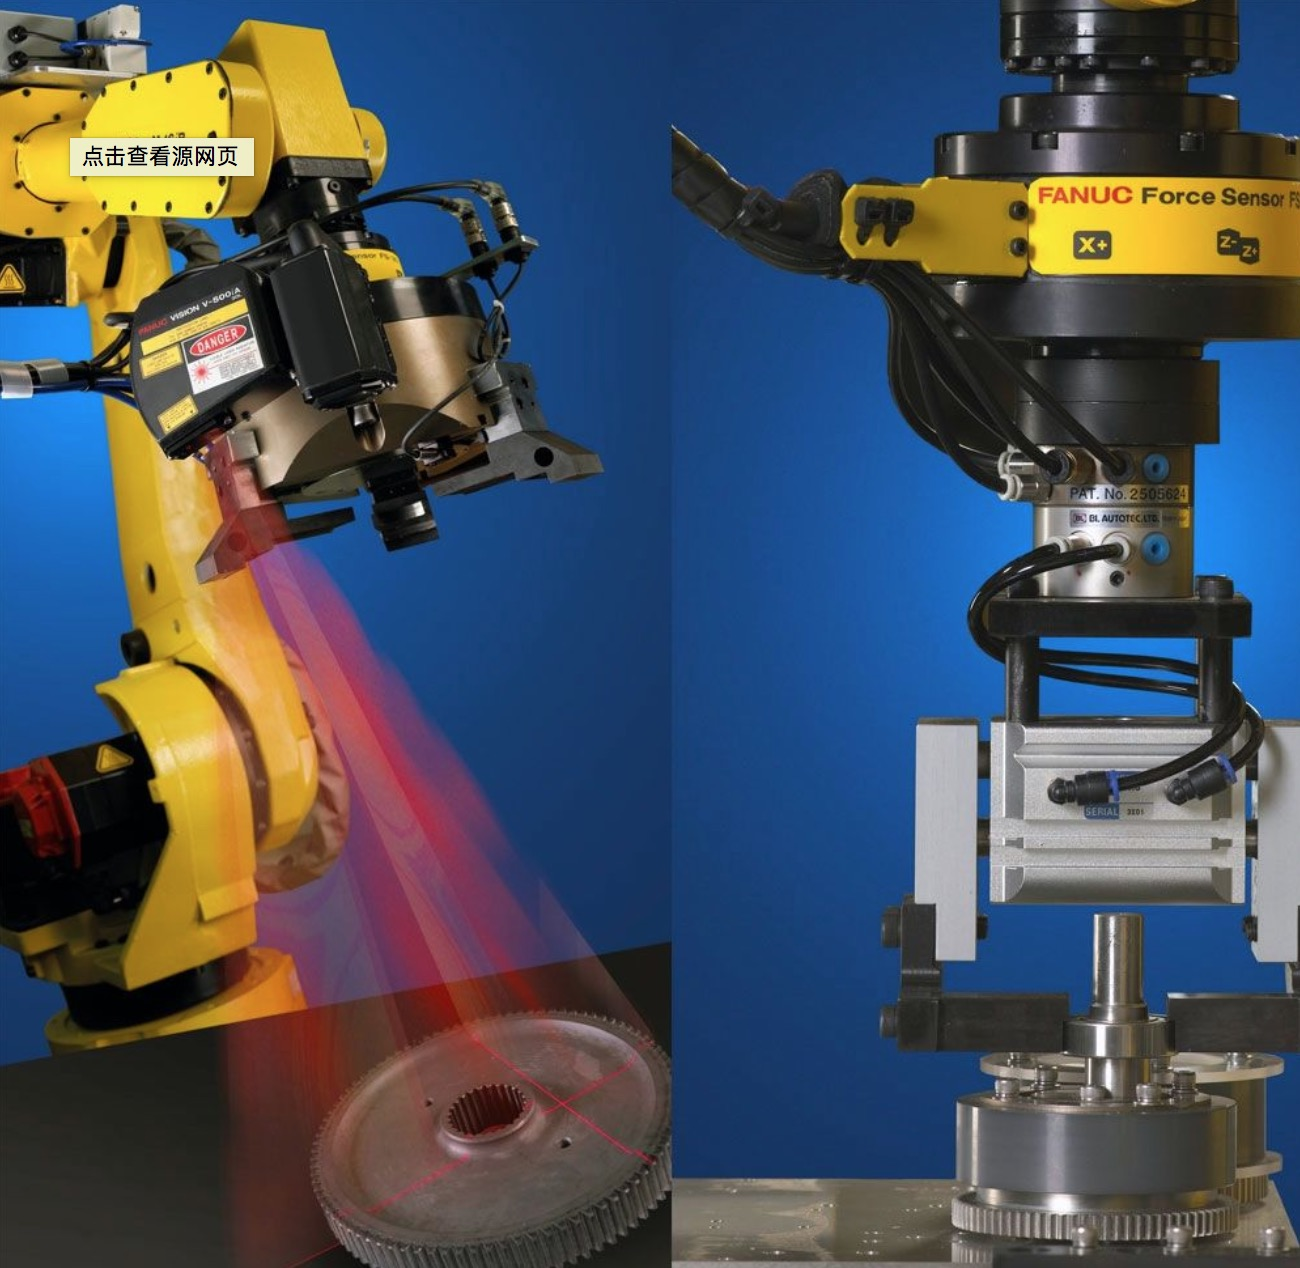
\includegraphics[scale=2.0]{./mypic/工业机器人2.jpg} 
		\end{minipage}}
	\subfigure[工业机器人抓取传送带盘上的零件]{ 
		\begin{minipage}[b]{0.5\textwidth} 
		\centering
		% \label{fig:SubFigure1} %% label for second subfigure 
		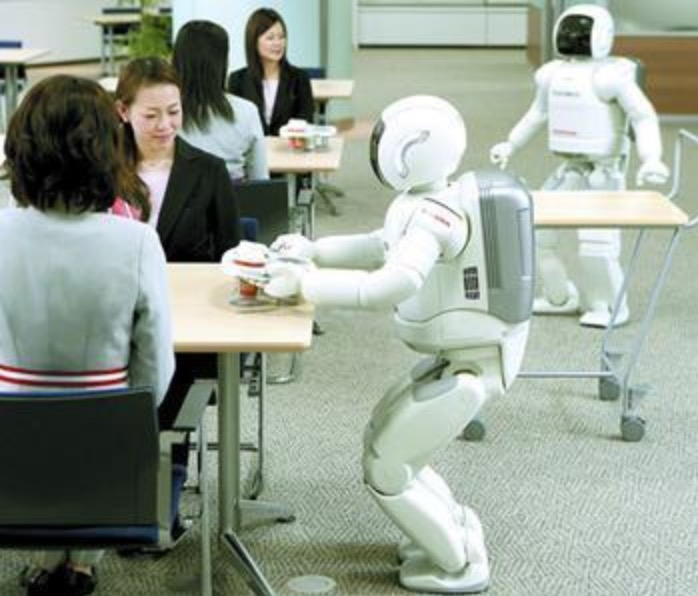
\includegraphics[scale=1.0]{./mypic/工业机器人1.jpg} 
		\end{minipage}}
	\caption{一些工业装配现场}
\end{figure}

在几乎所有工业环境中,计算机视觉是可以作为反馈的一种方便部署并且高效的方法。因此,计算机视觉已经成为了工业机器人研究领域中非常重要的一点。基于工业摄像头的计算机视觉是非常经典的研究内容,因为工业摄像头提供的高清RGB图像信息可以提供非常充足的环境信息,并且有很好的实时性。而近年来,伴随着例如Kinect,Leap Motion,RealSense等各种各样的面阵3D深度传感器的诞生,计算机视觉有了一个全新的维度。下图展示了一些常见的深度传感器。这些面阵3D深度传感器可以提供一个给定视角范围下工业场景的具有较高精度的深度尺寸信息,不再局限于只有RGB颜色信息的二维彩色图像上。并且这些3D深度传感器能在提供深度图像的同时给出与深度图像配准的RGB图像信息,也就是能够对空间中的物体同时进行颜色和深度的描述。这使得计算机视觉在感知上更接近于人眼,理论上可以观测到人眼所能观测到的所有信息。并且随着科技的发展,这些3D深度传感器的精度也在不断提高,传感范围也在不断扩大,其中Intel公司生产的RealSense传感器在近场工作环境下(20cm到120cm之间)精度可达1mm,完全可以应用于例如零件组装等特定工业场景中因此,针对这些3D深度传感器的计算机视觉研究掀起了一股热潮。

\begin{figure}[htb]
	\centering 
	% 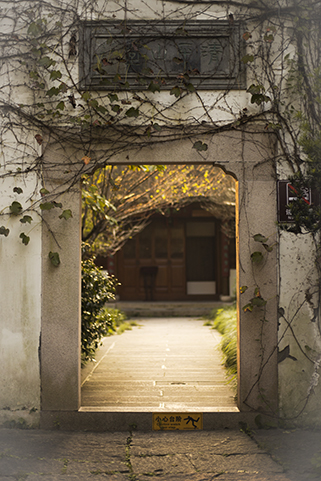
\includegraphics[width=\textwidth]{./Pictures/test.jpg} 
	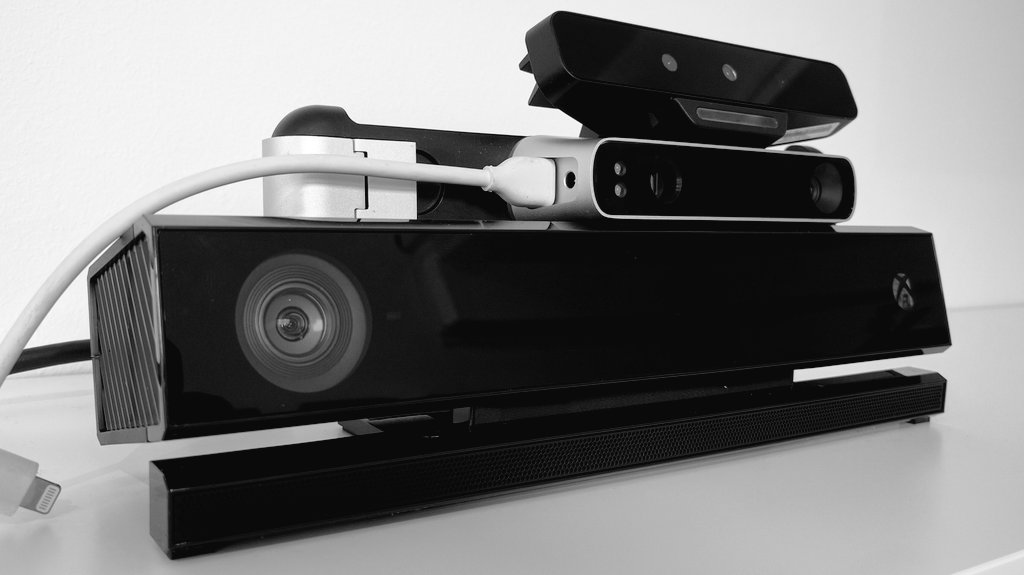
\includegraphics[width=0.8\textwidth]{./mypic/一些深度相机.jpg} 
	\caption{一些深度相机} 
\end{figure}


本文将在此背景下,面向工业装配演示编程中对物体位姿估计的需求,利用深度相机这一新型传感器展开研究和开发,以推动演示编程技术以及工业机器人的自动化发展。


\section{研究现状与趋势} 

物体位姿估计是一个非常大的领域。从目标角度来划分可以有人体姿势位姿估计、人脸特征点定位(五官位姿估计)、人脸朝向位姿估计、车牌位姿估计等各种其它实物的位姿估计。其中每一块内容都有非常多的研究人员投入,并且一直以来都有各种各样的方法和理论被提出,同时各个不同目标的位姿估计方法不断交融与碰撞产生更新颖更优秀的方法,持续促进着整个位姿估计领域整体的发展。但总体而言,物体位姿估计领域的各种优秀的方法可以被大致分为两种类型,一种是基于模版匹配的方法,另一种是基于模型回归的方法。两种方法各有优势也各有短处。

基于模版匹配的方法大致算法流程如下图所示。首先算法需要事先准备,或者事先计算好大量的模版,这些模版中每一个都代表被测物体的一个位姿状态。为了节省计算机资源和存储资源,这些模版在实际应用过程中将通过特征的形式进行存储,作为特征描述库。特征描述随算法不同而各不一样,常见的一些特征描述有SIFT\cite{lowe1999object},SURF\cite{bay2006surf},BRIEF\cite{calonder2010brief},ORB\cite{rublee2011orb}等经典特征描述。这些特征描述往往具有较好的尺度不变性以及对不同光照影响下的稳定性。存储好这些带有位姿信息等模版特征描述之后,便可以在实际位姿估计过程中通过比对输入的新图像的特征描述与特征描述库里的模版,得到一个最为接近的模版,从而最后得到对应的物体位姿。
\begin{figure}[htb]
	\centering 
	% 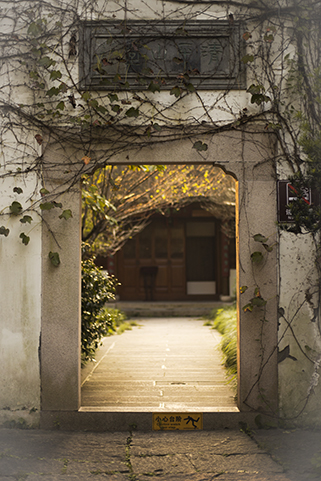
\includegraphics[width=\textwidth]{./Pictures/test.jpg} 
	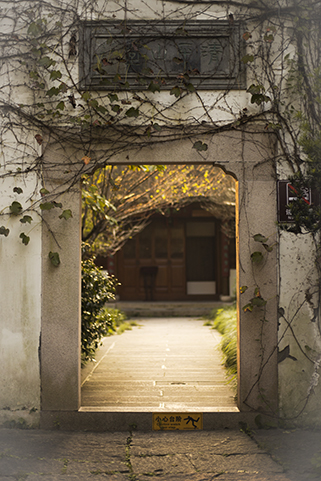
\includegraphics[scale=1.0]{./Pictures/test.jpg} 
	\caption{ljzst} 
\end{figure}

基于模型回归的位姿估计方法算法流程如下图所示。首先也是对目标物体进行特征提取,精准表达出物体的位姿特征。但是不同于基于模版匹配的算法框架,该方法在计算得到物体的特征描述之后不需要与实现准备好的模版库进行匹配,而是直接将位姿特征描述输入一个回归器里,通过回归器直接回归得到物体的位姿姿态。而其中这个位姿回归器则是通过事先大量的带真值标记的样本进行训练得到的。这其中的回归器可以是简单的线性回归,例如最小二乘回归等等,也可以是复杂的非线性回归例如SVM回归\cite{basak2007support}等。
\begin{figure}[htb]
	\centering 
	% 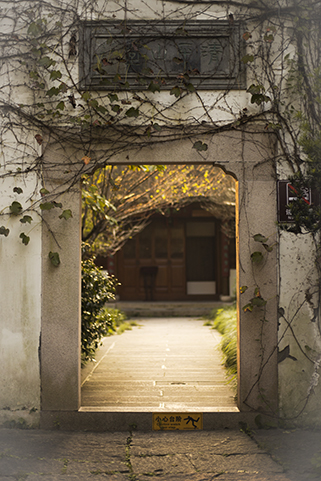
\includegraphics[width=\textwidth]{./Pictures/test.jpg} 
	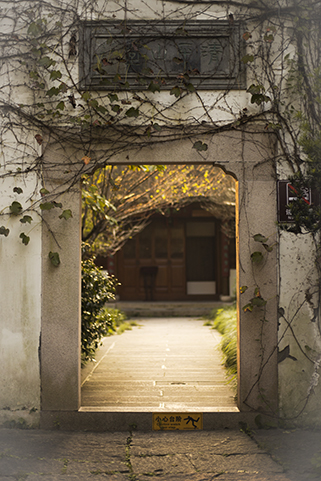
\includegraphics[scale=1.0]{./Pictures/test.jpg} 
	\caption{ljzst} 
\end{figure}

可以直观感受到,基于模版匹配的物体位姿估计方法通常需要较大的预存储空间,因为通常情况下一个物体的姿态会有非常大的变动空间,即使采用离散采样的方式来记录整个位姿空间下对应的各个位姿特征描述,也会有极大量的数据需要存储。一方面这样大量的存储会带来物理资源的需求,同时在进行位姿估计的过程中如果要匹配一对最接近的位姿特征描述,其计算量也是相当大的。相比之下基于模型回归的方法则有更为有竞争力。基于模型回归的方法虽然需要在事先通过学习大量的带标记的样本来得到物体的位姿回归器,但是位姿回归器在经过学习之后得到的模型通常只占有有非常小的数据存储空间。此外,当新的样本输入之后,位姿回归器根据其特征描述可以非常迅速地给出物体最终的位姿结果,不需要大量的计算资源。因此基于模型回归的位姿估计方法在实际应用过程中往往具有相对较强的竞争力。

在基于模型回归的位姿估计框架中,有很大一部分杰出的算法都用到了集成学习算法,并且考虑到位姿回归问题在回归空间上的高度复杂性,采用了非常新颖的级联回归算法进一步提高回归模型的回归能力。因此集成学习算法开始被大量关注并研究,同时级联回归算法框架也被不断应用到不同的领域当中。


\subsection{集成学习算法} % 随机森林与随机蕨 包括特征提取

集成学习方法通常指那些可以生成大量不同模型,并且可以将这些模型以一定的方式进行组合得到新的模型,从而用语解决分类或者回归问题\cite{mendes2012ensemble}。集成学习在很多情况下也被称为Committee、Classifier Fusion、Combination以及Aggregation等\cite{valentini2002ensembles}。从[\citenum{liu2000evolutionary}][\citenum{breiman2001random}][\citenum{rodriguez2006rotation}]等一些文章中可以看出,集成学习在近几年来取得了非常好的成绩,其优势具体表现在它相比单一的模型具有更加强大的鲁棒性以及准确性\cite{garcia2005cooperative}。其大致原理图如下所示:

\begin{figure}[htb]
	\centering 
	% 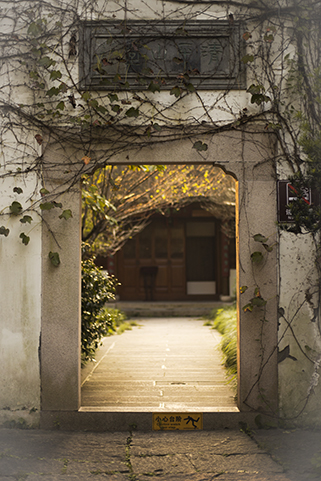
\includegraphics[width=\textwidth]{./Pictures/test.jpg} 
	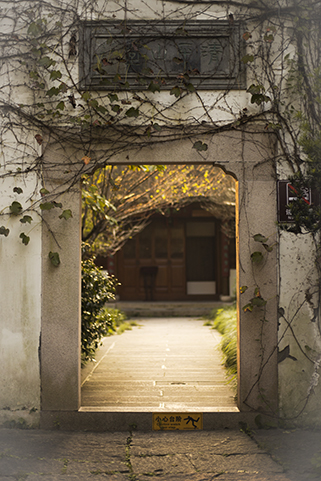
\includegraphics[scale=1.0]{./Pictures/test.jpg} 
	\caption{ljzst} 
\end{figure}


集成学习方法通过将不同模型进行组合得到新模型,按照这些子模型的种类关系可以将集成学习方法大致分为两种,分别是异态集成学习和同态集成学习。

异态集成学习是通过将种类不同的分类器进行集成,其中最为主要常见的两个主要方法为Wolpert等人提出的叠加法(Stack Generalization)\cite{wolpert1992stacked}以及Vilalta等人提出的元学习法(Meta Learning)\cite{vilalta2002perspective}。叠加法的思想是通过将基本的模型分布在多个层次上,再通过这个多层模型完成学习任务。William W等人在[\citenum{cohen2005stacked}]中则利用这种思想构造处了一种更加新颖的串行学习算法,并指出这种串行算法相比不串行在性能上有较大提升。元学习法的主要思想则是通过训练一个元模型来对所有的基本模型的输出进行进一步处理,最终得到问题输出结果。其主要包括两种方法:仲裁法(Arbiter)以及合并法(Combiner)。仲裁法是元模型从所有基本模型的输出结果中选择出合理的结果作为最后输出,例如投票方式。合并法则是通过用某种组合方法把所有基本模型的输出合并成最终输出,较为常见的Bagging\cite{breiman1996bagging}、Boosting\cite{schapire1990strength}等集成方法都是属于合并法。

同态集成学习方法则是指被集成的基本模型都应该属于同一种类的模型,仅仅只是这些基本模型之间的参数有所不同。同态集成学习模型主要有基于朴素贝叶斯的集成方法、基于决策树(Decision Tree,简称DT)的集成方法\cite{kearns1996boosting}、基于人工神经网络(Neuro-Network,简称NN)的集成方法\cite{zhou2002ensembling}\cite{zhou2002selectively}\cite{hansen1990neural}以及基于K—近邻的集成方法\cite{shen2007euk}等等。

异态集成学习方法由于需要提出众多不同模型才能构建更为强大的学习器,而通常情况下对于一个实际问题,要提出不同的模型来共同表述是一件非常困难的事情。相比之下,同态集成学习方法只需要提出一个简单的模型就可以完成复杂问题的学习。因此集成学习方法发展到现在,同态集成学习方法称为一种较为普遍并且表现优秀的一种学习方法,其中最为经典的一种同态集成学习方法就是随机森林\cite{breiman2001random}。随机森林算法是用随机的方式建立一个森林,森林里面有很多的决策树组成,随机森林的每一棵决策树之间是没有关联的。在得到森林之后,当有一个新的输入样本进入的时候,就让森林中的每一棵决策树分别进行一下判断,看看这个样本应该属于哪一类(对于分类算法),然后看看哪一类被选择最多,就预测这个样本为那一类。随机森林可以既可以处理属性为离散值的量,比如ID3算法,也可以处理属性为连续值的量,比如C4.5算法。另外,随机森林还可以用来进行无监督学习聚类和异常点检测。

与随机森林非常相似的另一个异态集成学习方法是随机蕨算法\cite{ozuysal2007fast}。随机蕨算法在2007年由Mustafa Ozuysal等人提出,并被广泛应用。其中最为出色的应用是在Zdenek Kalal等人提出的TLD跟踪算法中\cite{kalal2012tracking},该跟踪算法也称为深度学习大爆炸之前最为有名的跟踪算法之一。随机蕨算法表现出的优秀性质也被后来很多算法借鉴以及采用\cite{dollar2010cascaded}。

在众多优秀的集成学习算法中,本文希望能够挑选一种合适的学习算法,将其转变为适合物体位姿估计的集成学习方法。

\subsection{级联回归算法框架} % 人脸等在这里讲

在很多复杂回归问题中,级联回归算法是一种提高模型回归拟合能力的一种非常有效的方法。级联回归算法的初期想法由Jerome H Friedman等人在文章[\citenum{friedman2001greedy}]中提出。后来由Nigel Duffy等人经过研究在文章[\citenum{duffy2002boosting}]中进行了较为详细的叙述,将级联回归算法的核心思想以及能力进行了验证。随后经过大量的改进,SK Zhou等人将级联回归算法成功应用到了图像处理领域,这也奠定了之后一系列基于图像的级联回归处理算法基础\cite{zhou2005image}。

级联回归算法框架在各个应用场景下都得到了高度的认可,取得了不错的表现。在物体位姿估计领域,P. Doll{\'a}r等人在2010年提出了较为成熟稳定的一种物体位姿估计算法框架\cite{dollar2010cascaded}。在他们提出的文章中,采用了固定线性串流模型结构,通过将一系列回归器串联,每一级回归器充分利用上一层回归器的回归结果,不断补充回归器所能得到的输入信息,从而实现对回归目标更为精准的预测。如下图所示,首先算法需要一个目标所在的初始位姿,这个初始位姿不需要非常精准,然后算法通过对该初始位姿上的特征信息得到一个回归量用于矫正该初始位姿使其更加靠近真实位姿。
\begin{figure}[htb]
	\centering 
	% 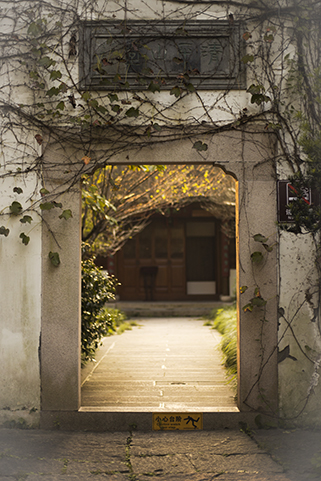
\includegraphics[width=\textwidth]{./Pictures/test.jpg} 
	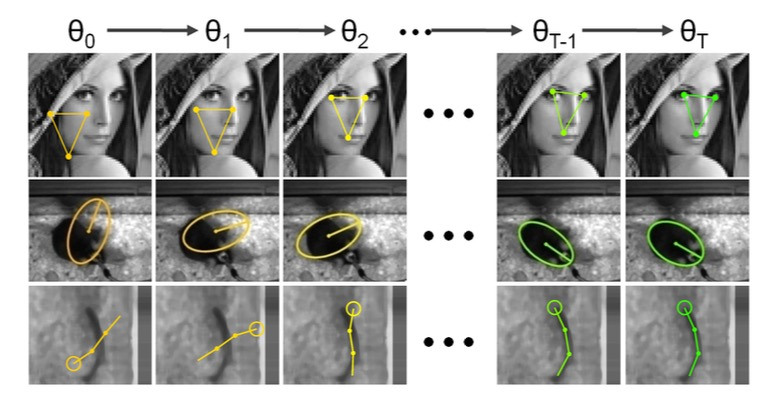
\includegraphics[width=\textwidth]{./mypic/级联回归.jpg} 
	\caption{图像上对物体位姿进行级联回归的一种基本框架} 
\end{figure}

级联回归算法在人脸特征点定位上取得的突破性进展是众多图像回归算法领域最为成功的一个。M. Dantone等人率先利用级联回归框架算法的高效性,并采用条件回归森林作为每一层的回归模型,得到了一种基于模型参数的实时人脸特征点定位算法,并取得了当时最精准的回归精度。同样借鉴于文章[\citenum{dollar2010cascaded}],X. Cao等人在2014年发表了一篇具有突破性意义的人脸特征点定位文章[\citenum{cao2014face}]。这篇文章中提出的人脸特征点回归算法采用非参数化的模型表达,通过直接估计人脸特征点在图像中的坐标位置来实现定位。这种通过直接减少特征点定位精度误差,而不是通过减少模型误差的方式,极大促进了回归精度以及回归速度。能有这样显著的效果提升,极大程度上依赖于级联回归框架的高拟合能力。随后P. Doll{\'a}r再一次总结X. Cao等人的工作经验,利用自己提出的级联回归框架,提出一种能够适应一定人脸被遮挡情况下的人脸特征点定位算法,再一次提高了人脸特征点定位的精准度\cite{burgos2013robust}。在期间也有相关的一些相关的神经网络回归算法被应用到这个领域,但是经过实验证明,神经网络的回归能力和级联回归算法框架下差别不大,但是在计算效率上则远不及级联回归算法\cite{sun2013deep},随后也被慢慢淘汰。最后在[\citenum{ren2014face}]文章中,R. Shaoqing等人提出了一种里程碑意义的人脸特征点定位算法。在该算法中,通过提出局部二值特征,并以级联回归学习框架对人脸特征进行学习,从而引导回归模型进行拟合,最后得到了具有极高精度,极高速度并存的人脸特征点定位算法。于此同时,类似文章[\citenum{cootes2001active}][\citenum{saragih2009face}][\citenum{yang2014face}][\citenum{asthana2014incremental}][\citenum{kazemi2014one}][\citenum{burgos2013robust}][\citenum{xiong2013supervised}]也通过类似的级联回归框架在人脸特征点定位领域取得了相当优秀的成果,具有很高学术借鉴意义。

人脸特征点级联回归回归算法的大致框架可以如下图所示:
\begin{figure}[htb]
	\centering 
	% 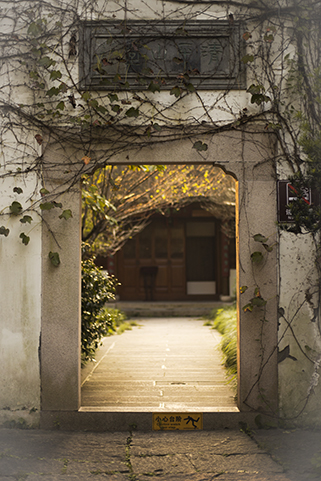
\includegraphics[width=\textwidth]{./Pictures/test.jpg} 
	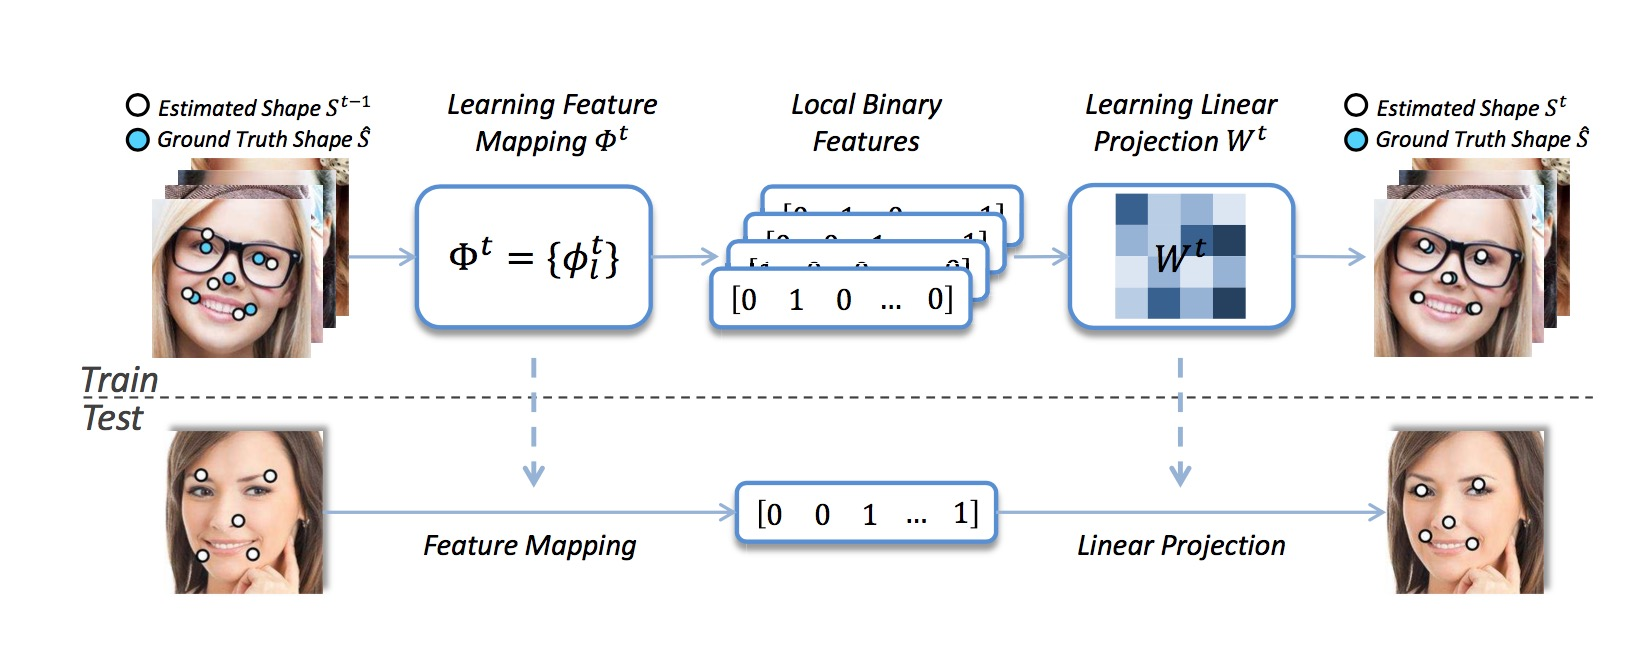
\includegraphics[width=\textwidth]{./mypic/人脸回归算法框架.jpg} 
	\caption{人脸特征点定位问题中的级联回归算法框架} 
\end{figure}
首先在训练模型阶段,学习计算出当前特征点处的特征描述,并以此作为下一级回归器的输入,而当前特征点位置与真值之间的偏移量作为下一级回归器的目标回归量。通过大量的真值样本进行训练得到下一级回归模型。此处特征点的位置可以由目标检测器初始化给出,或者是通过上一级的回归模型得到修正之后给出。重复上述过程就可以得到级联回归模型。而在实际测试应用中,通过计算当前特征点位置的特征描述作为当前级拟合回归模型的输入,得到当前目标回归矫正量。将该矫正量叠加到上级特征点位置后可以得到更新后的特征点位置。重复上述过程,完成所有级联回归模型的拟合修正就可以得到最后的人脸特征点位置。这样的模型非常简洁,但具有非常强的拟合能力,能够适应像人脸特征点定位这样具有非常高复杂度回归空间的回归问题,证明了级联回归模型具有相当优秀的实际应用价值。因此本文也希望充分利用这样的级联回归框架,对物体的六维位姿估计问题展开研究。

\subsection{物体的六维位姿估计}

物体的六维位姿估计一直以来是机器人领域一个基础问题。早期物体位姿估计的算法研究都是基于工业相机展开的。其中较为成功的几种算法有M. Jones提出的一种基于全局表面特征的位姿估计方法\cite{jones2003fast},以及一些基于局部表面特征的位姿估计方法\cite{schmid1996combining}\cite{rothganger20033d}。随后,D. Thachasongtham等人提出一种更为鲁棒的算法框架,通过事先仿真物体在三维空间中的各个位姿,并通过训练筛选出各个空间位姿下该物体具有的最为稳定的特征点以及相应的特征描述,最后在线测试时通过这些稳定的特征点进行三维位姿匹配\cite{thachasongtham20133d},这样的算法在当时具有一定的大角度变动适应性以及对一些遮挡情况有较好的表现。文章[\citenum{hara2014growing}]研发了一种增长回归随机森林用于对物体的位姿进行直接预测,但是该增长回归森林算法仅仅可用于分类问题,也就是对物体的直接位姿估计是不够精准的,需要后续其他迭代算法对其结果进行调优。

近些年来,随着深度相机的不断发展,各种新型的深度传感器给机器视觉带来了更丰富的信息来源,深度相机引发了一次物体位姿估计的研究热潮。文章[\citenum{germann2007automatic}]搭建了一个3D仿真环境,用于渲染3D模型在空间中的各个位姿,并利用这个仿真提取一些标准深度图像模版,最后通过在线匹配这些深度图像模版与实际深度相机采集到的深度图像进行位姿估计,初步实现了深度图像下的物体六维位姿估计。但由于这个版本的算法需要极大的计算量,文章作者利用GPU进行并行加速计算提高效率,但仍旧无法实现较快的结果输出。随后M. Germann等人改进了其算法,通过简化标准模版之间匹配的过程,同样利用GPU并行处理,提高了该算法框架的实时性,效果得到了显著提升\cite{park2010fast}。下图为该类算法一个简易框架示意图,其中最后调优过程一般采用ICP(Iterative Closest Point)算法。
\begin{figure}[htb]
	\centering 
	% 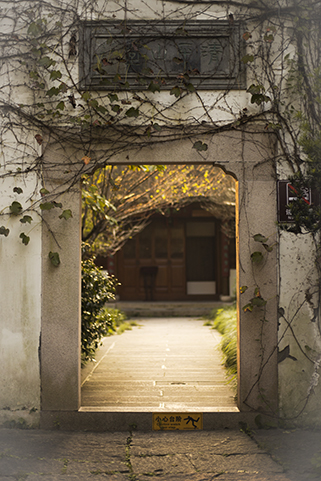
\includegraphics[width=\textwidth]{./Pictures/test.jpg} 
	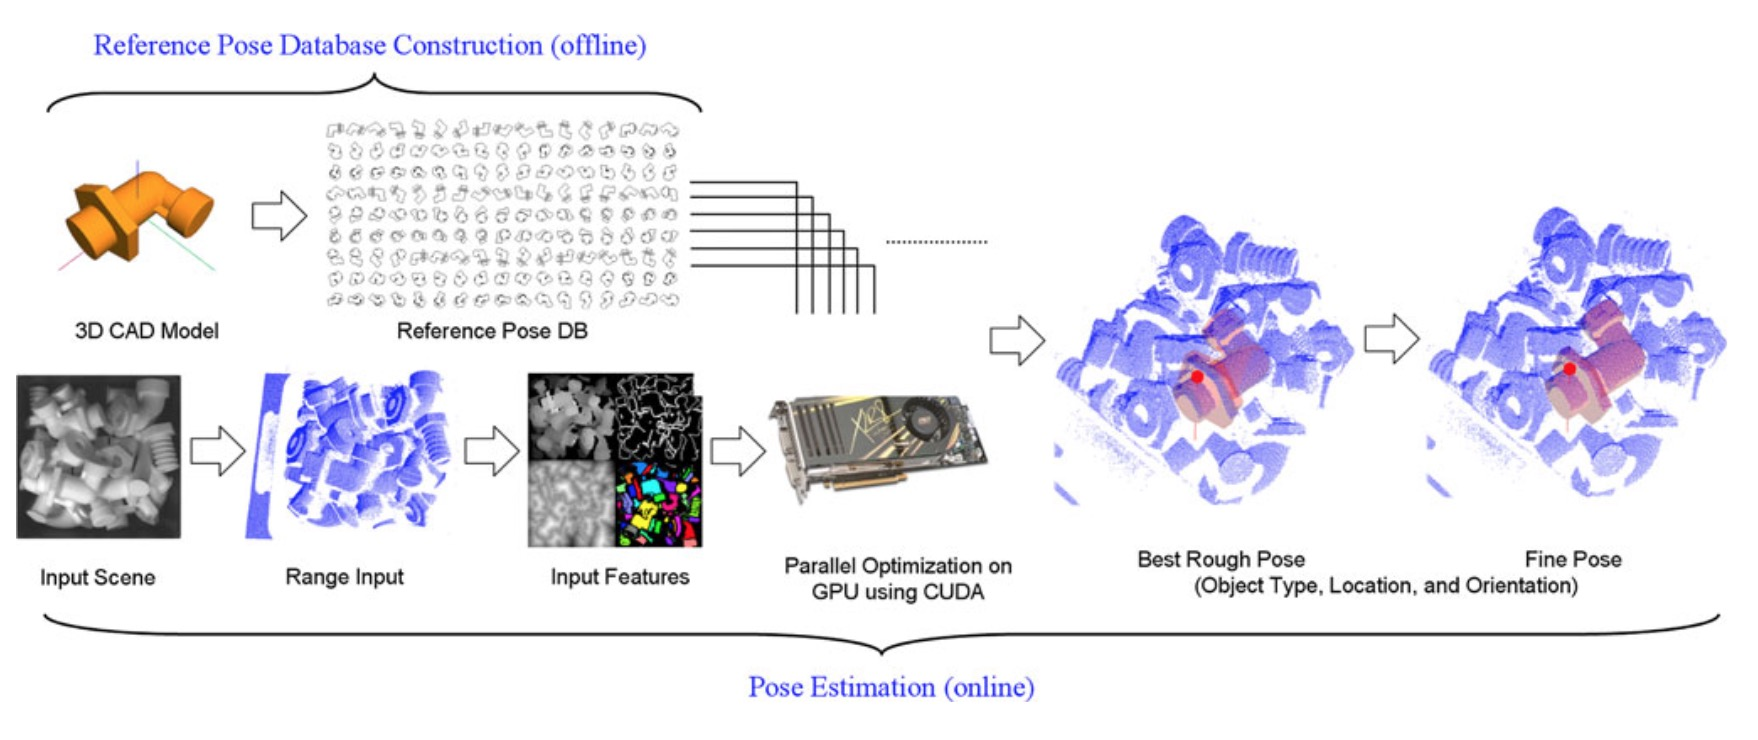
\includegraphics[width=\textwidth]{./mypic/早期位姿估计算法框架.jpg} 
	\caption{早期位姿估计算法框架} 
\end{figure}

为了提高物体位姿估计的实时性,B. Drost等人提出一种基于点云法向量的全局模型特征PPF(Point Pair Features)。这种特征包含了所有模型点云对之间的特性并且与整个模型之间存在一种配对关系,同时具有非常好的计算效率\cite{drost2010model}。利用这种特征描述进行投票机制的位姿估计,使其算法具有非常好的速度以及精度表现。另外S. Hinterstoisser等人则直接利用深度图像计算其对应的梯度响应图作为其特征匹配的基础,得到了非常好的位姿估计效果,同时其计算实时性也非常高\cite{hinterstoisser2012gradient}。他们提出了一种叫做LINE(LINEearizing the memory)特征,包含仅用于深度图像的LINE-2D特征、用于深度图像表面法向量的LINE-3D特征以及用于多模型的LINE-MOD特征。这些特征描述具有非常好的表达能力,是深度图像特征中非常实用的方法。之后他们利用这些特征又提出了一种多模版匹配算法,用于复杂环境下的物体位姿估计,并取得了相当好的效果\cite{hinterstoisser2011multimodal}。

在文章[\citenum{tang2014latent}]提出潜回归随机森林以及文章[\citenum{gall2011hough}]提出霍夫随机森林这两个相当优秀的回归森林算法之后,A. Tejani等人结合这两种算法,提出一种新颖的潜类别霍夫随机森林算法,同时结合LINE-MOD特征用于物体的检测以及六维位姿估计\cite{tejani2014latent}。该算法在当时表现相当出色,取得了State-of-the-art效果。于此同时,E. Brachmann等人采用能量谱图结合随机森林投票的方式也取得了不错的结果,具有较好的借鉴意义\cite{brachmann2014learning}。

随着深度学习的出现和流行,一些基于深度学习的物体位姿框架也逐渐被提出。P. Wohlhart等人提出的一种深度学习特征提取框架能够得到相比LINE-MOD特征更好的特征表述\cite{wohlhart2015learning}。但受限于深度学习框架的庞大性,很难实现高效便捷的算法部署,因此类似的利用深度学习框架进行位姿估计的算法研究成果大都不是特别理想。

得益于人脸特征点定位取得的优秀成果,X. Sun等人将人脸特征点定位算法进行移植改造应用于人手掌的位姿估计中,取得了相当优秀的成果\cite{sun2015cascaded}。该算法通过给手掌指定一些关键点,并设计了一种能适用于深度图像的特征描述方式进行级联回归,能够在不利用GPU并行加速计算的情况下对手掌进行实时位姿估计,同时具备相当准确的位姿回归精度。下图是该算法的一个简单流程示意图:
\begin{figure}[htb]
	\centering 
	% 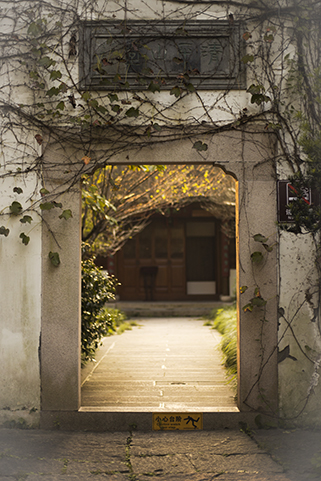
\includegraphics[width=\textwidth]{./Pictures/test.jpg} 
	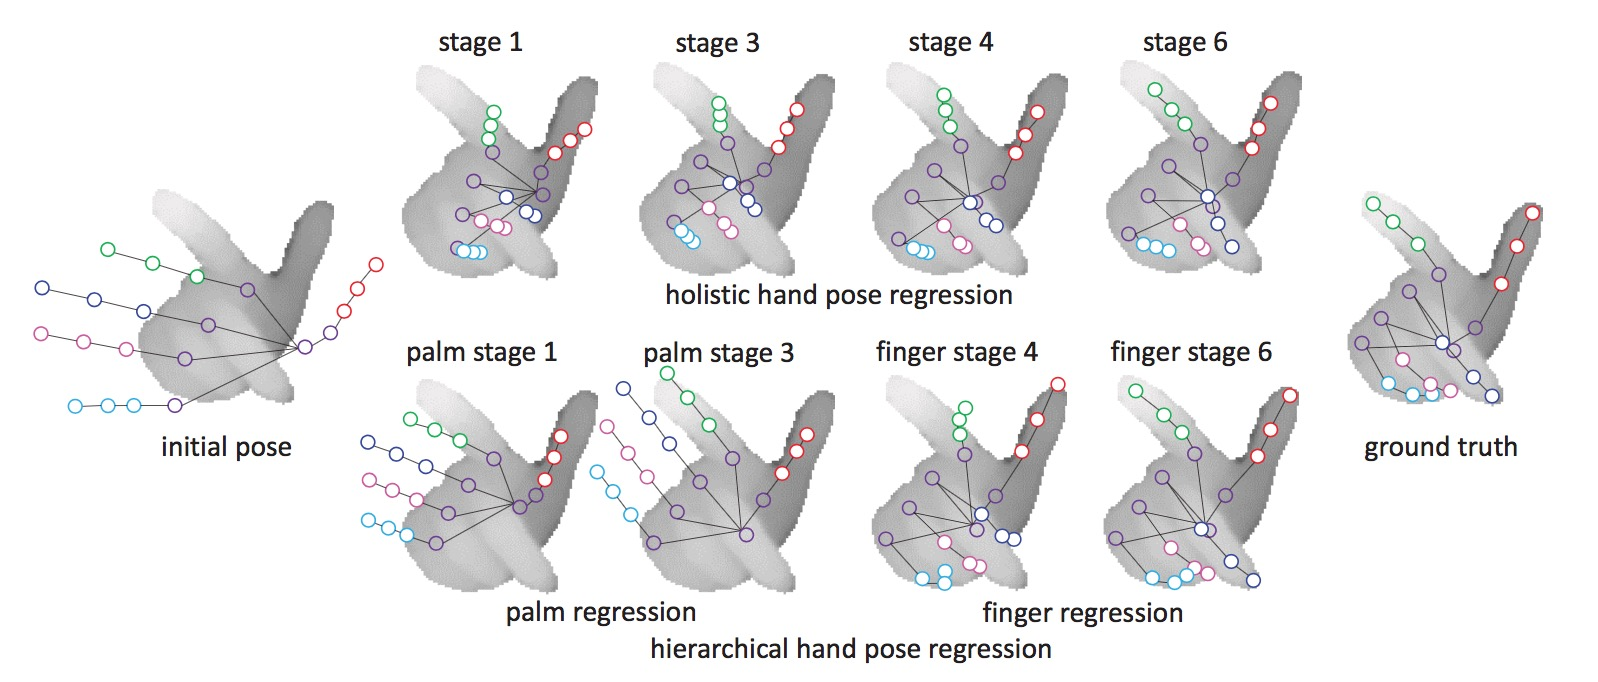
\includegraphics[width=\textwidth]{./mypic/手掌位姿估计流程示意图.jpg} 
	\caption{手掌位姿估计流程示意图} 
\end{figure}
首先在深度图像中给定一个任意的手掌初始位姿,然后通过对关键点的深度图像特征提取,结合随机森林算法进行级联回归最后得到准确的手掌位姿。类似的,E. Brachmann也采用了级联回归框架进行了对通用物体的位姿估计研究,采用RGBD相机作为借口实现了较为理想的位姿估计结果,但在计算效率上略有降低\cite{brachmann2016uncertainty}。这些工作指引物体位姿估计研究的重点放在了级联回归框架上,随后R. Kouskouridas等人进一步改进潜类别霍夫随机森林,实现了物体六维位姿估计高精度情况下的又一次性能提升\cite{kouskouridas2016latent}。

总体而言,物体位姿估计研究在朝着高效率高精度的方向发展。但首先于目前深度相机的精度还并没有非常高,所以目前的研究主要是通过改进算法框架,实现一个更易部署,更为高速的物体位姿估计算法。因此文本也希望能够进一步提高物体位姿估计算法的效率,同时保证其有较好的精度。

\section{本文研究内容}

工业装配演示编程的背景下,物体的六维位姿估计研究具有如下几个特点:
\begin{itemize}
\item 工业现场需要进行物体位姿估计的场合中,这些物体往往是具有严格尺寸信息的规则刚体,一般都有精确的3D模型。
\item 工业现场很多零件日新月异,每当有一个新的零件需要投入生产时都需要对流水线过程进行更新,或者物体位姿估计算法更新。
\item 工业现场追求效率,所有的应用算法都需要有较高的实时性从而提高生产效率。
\end{itemize}
针对上述这几个现实问题,本文思路为通过继续深入研究随机森林等集成学习算法,进一步提高这类算法的适用性以及鲁棒性,从而使其应用于物体位姿估计领域时能有更好的表现。另一方面为了使物体位姿估计算法具有更好的通用性以及更好的易部署性,本文将考虑利用现有工业条件搭建一个物理仿真环境,方便物体位姿估计算法的快速实现。最后结合级联回归框架得到一个较为完善的工业场景下的物体六维位姿估计方案。

本文最终得到的研究内容可以分为下面这三个大块:
\begin{itemize}
\item 首先以人脸特征点定位这个较为成熟的研究平台来验证随机蕨回归算法的可靠性,以及随机蕨回归算法在面对高维回归空间问题的回归能力和效率。并通过修改经典随机蕨回归框架,通过给算法输入增加一个掩码接口,实现随机蕨回归算法能够有更强的适应性,在针对特征不完备情况下的回归也能合理进行。最后通过实验验证该算法的可行性。
\item 充分利用工业现场可以提供的零件的3D模型信息,借助OpenGL软件平台搭建一个深度相机仿真平台。通过模拟零件在相机视角下的各个位姿,并添加对应的背景以及前景信息,在短时间内生成大量的仿真数据用于后续对物体位姿估计模型的训练。同时,本文将通过修补深度相机产生的空洞以及为仿真深度图像添加随机噪声使其与真实深度图像更为接近,提高仿真程度。
\item 借鉴人脸特征点定位以及文章[\citenum{sun2015cascaded}]中的思路,针对工业现场零件的位姿估计问题设计全新的物体六维位姿级联回归算法框架。并通过设计新的深度图像特征实现物体六维位姿估计算法的高效性。最后利用改进后的随机蕨回归算法,通过对物体的遮挡情况进行估计,实现当物体存在部分被遮挡情况下也能得到较为理想的物体位姿估计结果。
\end{itemize}


\section{本文结构安排}

本文结构安排如下:

第一章主要介绍了在工业环境下本文针对物体位姿估计研究的背景以及意义,并给出了当前集成学习、级联回归算法以及物体六维位姿估计等领域的研究现状。随后给出了本文的主要研究内容以及结构安排。

第二章中先给出了随机蕨算法的经典定义,并通过改造随机蕨算法中的推理公式改造为可以用于回归问题的随机蕨回归算法。然后结合实际应用问题,进一步改造随机蕨算法将其结合特征掩码,介绍如何将随机蕨算法应用到有大噪声干扰的情况中去。最后通过实验验证这些算法改进之后的合理性以及可行性。

第三章主要介绍了在搭建仿真深度相机过程中的数学模型,以及仿真环境搭建的主要流程。其中包括仿真环境中的坐标系设定、旋转关系、OpenGL中的一些基本原理等。并通过进一步为仿真深度图添加人工噪声以及前景背景信息增强其仿真真实度。最后在实验中给出仿真环境的一系列结果。

第四章首先提出了一种可以用于深度图像上的特征提取办法,讨论其尺度不变性,并利用一种监督学习下的特征降维办法对特征进行信噪比提高。然后针对物体的位姿估计提出一种级联回归框架,使其能够实现对通用物体的六维位姿估计。接着进一步讨论物体在存在遮挡情况下如何利用扩展功能后的随机蕨进行针对性处理,以实现复杂环境下的物体位姿估计。最后在本章实验环节中给出了该物体位姿估计算法的可行性以及准确性分析。

第五章给出了本文研究过程中的一些总结,以及对之后的研究工作作出展望。















\chapter{随机蕨算法的改造与应用}

\section{概述}

随机蕨算法是随机森林算法的一种变种,也是基于传统贝叶斯理论提出的一种集成学习方法,
最早由Mustafa Ozuysal等人提出\cite{ozuysal2007fast}。
随机蕨和随机森林的区别主要有如下这四个方面:
\begin{itemize}
\item
随机森林算法直接学习后验概率,
而随机蕨算法则是通过学习类别条件概率密度分布
\item
在随机森林算法中,对于每个输入样本,比较的特征次序会有所不同,
但是在随机蕨算法中,对于每个输入的样本比较的特征的次序都是相同的。
\item
在训练过程中,随机森林算法的训练时间是随着随机树的深度指数增长,
而在随机蕨算法中,训练时间仅仅随着数的深度呈线性增长。
\item
在随机森林算法中,算法的最后结果是通过对每个决策树的加权平均来得到的,但是在随机蕨算法中,最后结果则是以贝叶斯规则综合得到。
\end{itemize}
% \begin{itemize}
% \item
% 随机森林算法直接学习后验概率$P(C_k|F)$,
% 而随机蕨算法则是通过学习类别条件概率密度分布$P(F|C_k)$
% \item
% 在随机森林算法中,对于每个输入样本,比较的特征次序会有所不同,
% 但是在随机蕨算法中,对于每个输入的样本比较的特征的次序都是相同的。
% \item
% 在训练过程中,随机森林算法的训练时间是随着随机树的深度指数增长,
% 而在随机蕨算法中,训练时间仅仅随着数的深度呈线性增长。
% \item
% 在随机森林算法中,算法的最后结果是通过对每个决策树的加权平均来得到的,但是在随机蕨算法中,最后结果则是以贝叶斯规则综合得到。
% \end{itemize}
% 其中,$P$表述算法最后的概率输出结果,$C_k$表示算法分类器的目标类别,$F=\{f_1,f_2,...,f_N\}$表示输入算法的特征,下文同。
随机蕨算法经过实验验证,在相同层数的情况下,具有比随机森林更为优秀的分类能力以及抗过拟合能力,同时在计算效率上与随机森林不分上下,仅仅在模型存储上有较高的需求。因此随机蕨凭借出色的表现,得到了越来越多的关注。

但随机蕨算法目前的讨论都是在分类问题的基础上进行的,算法最后的结果也是在给定类别数目的情况下才能实现。但是在很多实际问题中,往往遇到的是回归问题,需要求解的目标空间往往是连续的,这个时候上述方法将不再适用。本文针对这样的情况,结合随机蕨的特性,借鉴随机森林算法改造应用到拟合回归问题中的方法,将随机蕨算法加以改造,使其也能适用于拟合回归问题。在此基础上,本文将进一步扩充随机蕨算法,通过增加一层掩码机制使其在输入特征有较大噪声的情况下也能有较强的鲁棒性,使算法能够在更多的应用场景中有更稳定的表现。

本章结构安排如下:节2.2介绍随机蕨算法通过修改输出函数表达式可以实现其在拟合回归问题中的应用。节2.3将介绍如何将掩码添加进随机蕨算法框架中,从而实现随机蕨算法在对抗大噪声情况下仍然具有较强的鲁棒性。最后在节2.4,本文通过将随机蕨算法应用到人脸对齐问题中,通过实验验证了改进后的随机蕨算法在回归问题中的可行性以及相比于普通拟合算法的鲁棒性,说明了该改进算法具有较强的实用性。



\section{随机蕨算法基本原理}
本节简要阐述一下随机蕨算法的具体原理。对于一个分类问题,需要计算各个类别间的概率分布:
\begin{equation}
	\arg\max_{k} P(C_k|f_1,f_2,...,f_N)
\end{equation}
其中,$P$表述算法最后的概率输出结果,$C_k$表示算法分类器的目标类别,$F=\{f_1,f_2,...,f_N\}$表示输入算法的特征。在贝叶斯规则下,上式等价于:
\begin{equation}
	\arg\max_{k} P(f_1,f_2,...,f_N|C_k)P(C_k)
\end{equation}
该式子表明一个后验概率与先验概率密度与相似函数的乘积成正比。然而对于一个高纬度的特征描述,或者说一个复杂的决策树输入样本,是很难计算出或者学习出相关联的相似度分布。或者说计算高维度的相似度分布是一件非常耗时耗资源的工作,在很多计算资源有限、计算实时要求高的应用场景中,计算高维特征相似度变得非常笨重,$P(f_1,f_2,...,f_N|C_k)$会非常难以求解。但如果假设在给定了目标类别的情况下,特征的各个维度之间是有一定的相互独立性的。这个时候,朴素贝叶斯理论可以对上述公式有如下简化:
\begin{equation}
	P(f_1,f_2,...,f_N|C_k)=\prod_{i=1}^N P(f_i|C_k)
\end{equation}
从而目标类别表达式为:
\begin{equation}
	Class(F)\equiv \arg\max_k P(C_k)\prod_{n=1}^N P(f_n|C_k)
\end{equation}
但这个独立性的假设在大多数的情况下是很难成立的,大多数情况下,上式得到的概率结果会小于真实的后验概率。为此,需要进一步假设。假设高维特征可以分解为几个小特征组合,并且这些小的特征组合之间是几乎完全相互独立的。这个假设在很多情况下都可以满足实用性。例如原始特征$F$分解为L组,每一组的特征大小为S,则有:
\begin{equation}
\begin{aligned}
	F=\{F_1,F_2,...,F_L\} \\
% \end{equation}
% \begin{equation}
	F_l=\{f_{l_1},f_{l_2},...,f_{l_S}\}
\end{aligned}
\end{equation}
当L组特征间相互独立假设下:
\begin{equation}
	P(f_1,f_2,...,f_N|C_k)=\prod_{l=1}^L P(F_l|C_k)
\end{equation}
于是可以得到最后的类别概率分布:
\begin{equation}
	Class(F_l)\equiv \arg\max_k P(C_k)\prod_{l=1}^L P(F_l|C_k)
\end{equation}
上式就是随机蕨算法的根本,采用半朴素贝叶斯的方式,平衡了算法计算的复杂性以及算法的准确性。其中每一个特征组构成的决策树被称为一个蕨,实际应用过程中,通过调整蕨的大小(也就是$S$的大小),就可以实现对算法复杂性以及准确性的控制。图2-1为该经典随机蕨算法的示意图。
\begin{figure}[htb]
	\centering 
	% 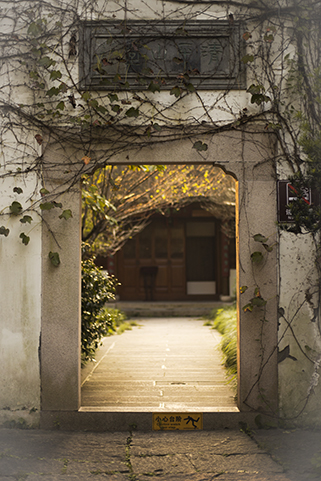
\includegraphics[width=\textwidth]{./Pictures/test.jpg} 
	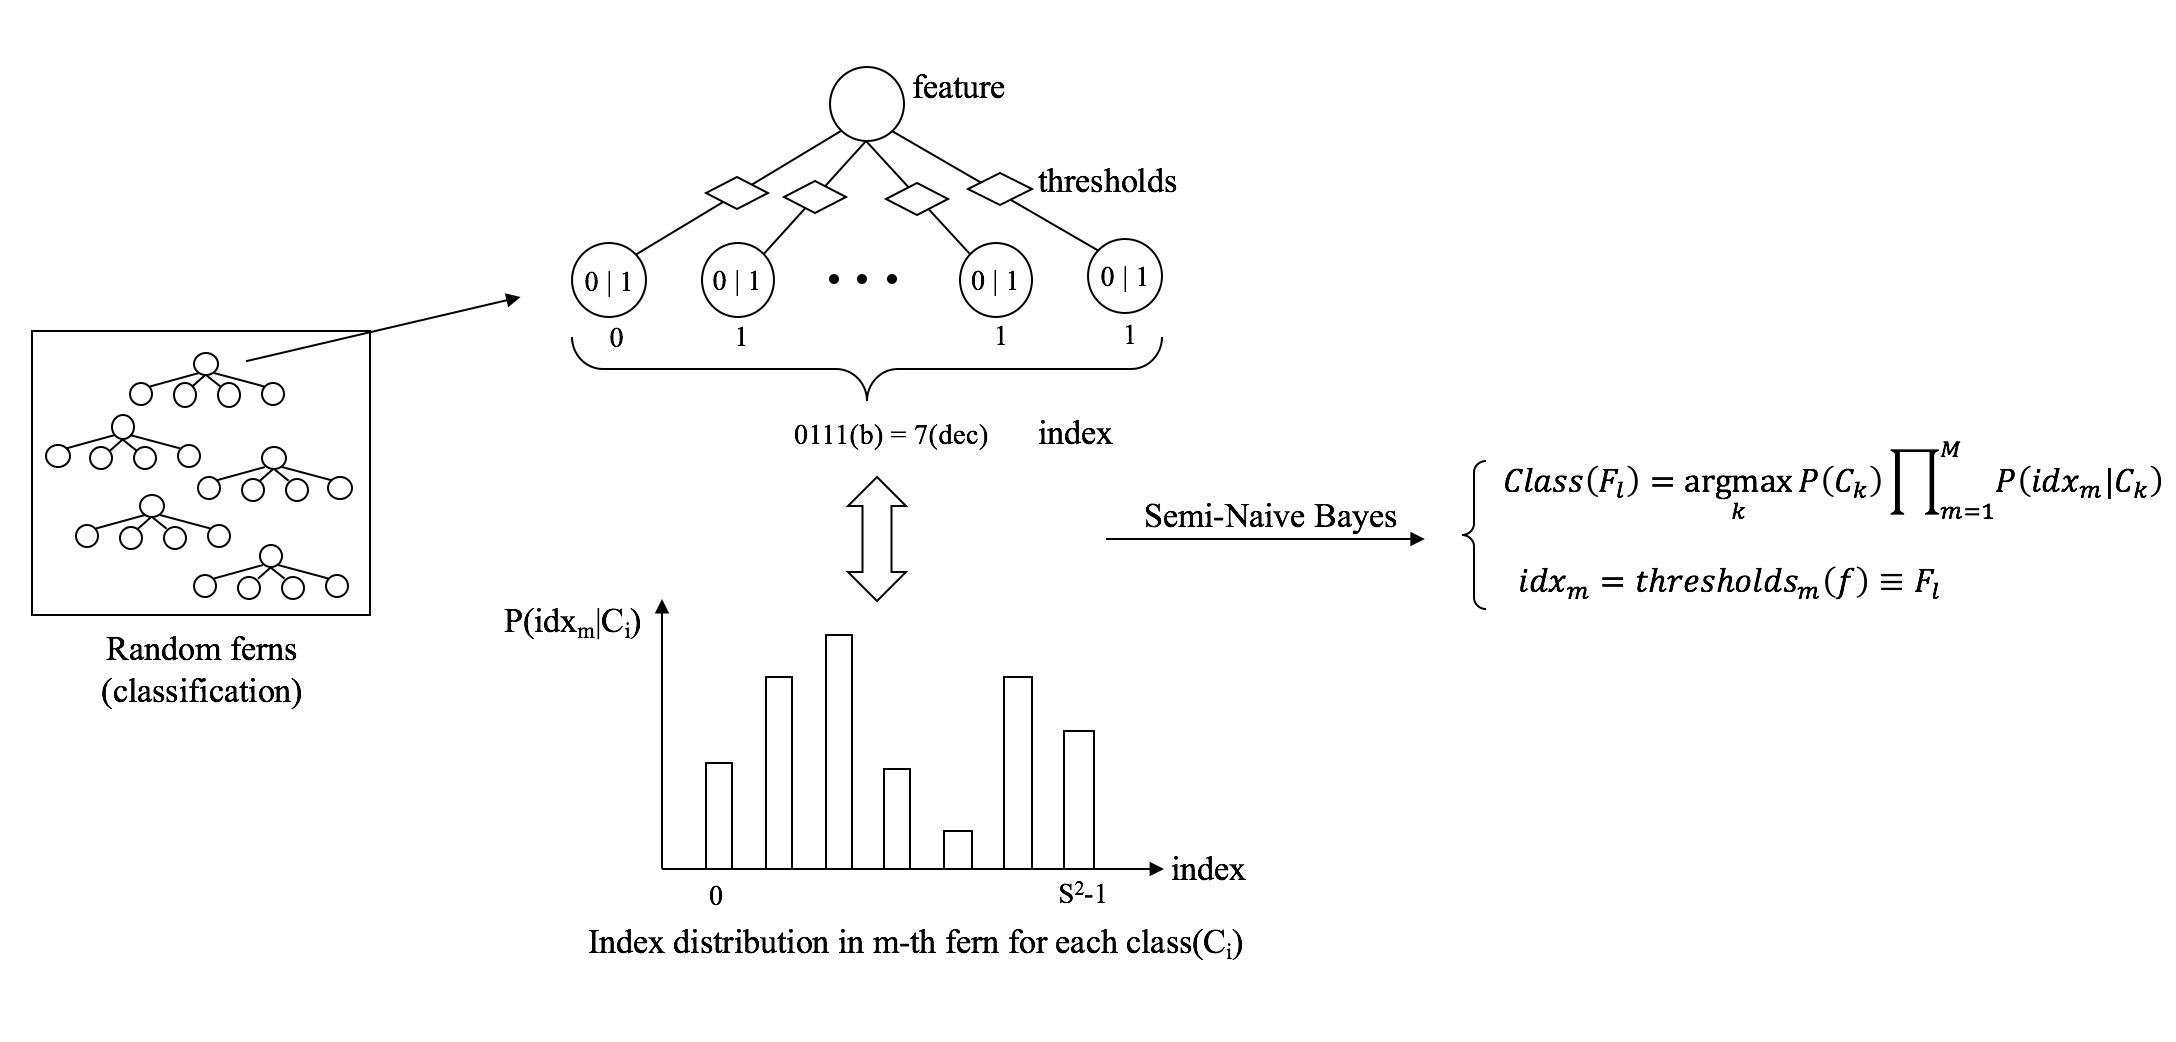
\includegraphics[width=\textwidth]{./mypic/经典随机蕨算法的示意图.jpg} 
	\caption{面向分类问题的经典随机蕨算法示意图} 
\end{figure}



\section{拟合回归问题下的随机蕨算法}
在分类问题下的随机蕨算法中,每个决策树的叶子节点记录的是所有落到该叶子节点的样本的类别概率分布均值。该模型在遇到新的输入样本后,将根据样本最后落入的叶子节点,统计所有叶子节点的概率分布均值来计算该样本的最后分类结果。这个模型显然不适用于回归问题。随机蕨算法被用于解决回归问题的思想最早在文章[\citenum{dollar2010cascaded}]中提出,后来也被应用到人脸对齐问题中\cite{cao2014face},但是都没有对其进行详细的说明阐述,很多算法实现细节被隐藏了。因此,本文将根据自己的理解和对算法的改善在此重新整理。

假定所有的输入样本都具有相同的特征维度$N$,$F=\{f_1,f_2,...,f_N\}$,以及相同$P$维度的目标回归空间$Y=\{y_1,y_2,...,y_P\}$。

首先任意地随机选取$S$个输入特征维度$(S<N)$,并随机生成$S$个阈值。将训练数据的这$S$个维度与这$S$个随机阈值进行简单大小比较,理想情况下可以得到$2^S$种不同的情况,同时对应地生成$2^S$个索引码。对这$2^S$个类别下的训练数据,我们计算其类内的均值,并记录为$L:\{L_1,L_2,...,L_{2^S}\}$,这样我们就得到了一个最简单的蕨。对于这个蕨,每次输入一个新的样本,仅仅需要将这个新的样本中那对应的$S$个维度上的数值与这$S$个阈值进行比较,就可以得到一个分类索引,然后只要根据这个索引在$L$中找到对应的均值记录(假定索引值为$i$),取出该均值便可以得到新样本的回归拟合值$L_i$。

这个基础蕨具有非常弱的拟合能力,甚至在随机阈值非常极端的情况下有可能完全不具备拟合能力。因此,我们需要重复这个随机过程(包括选取随机维度和生产随机阈值)多次,并记录下每一次随机过程的结果,并用损失函数来衡量这个随机过程得到的基础蕨的质量。损失函数可以有很多,例如:
\begin{equation}
	Loss=\sum_i{\|L_i-\overline{L_i}\|}
\end{equation}
如果某一次得到的损失函数值在所有随机过程中为最小,则抛弃所有其它的随机过程,用这次随机过程中选取的随机维度和随机阈值作为这个基础蕨的最终模型。记录维度信息$dim$、阈值信息$thresh$以及该阈值下的样本类别均值$L$。

这样的重复随机过程在经历一定量的次数之后将会大大加强该基础随机蕨的拟合能力,但是受限于随机过程的可重复次数,以及基础蕨的分类能力仅仅能实现$2^S$个,也限制了该基础蕨的拟合能力上限。因此,为了继续提高随机蕨算法的拟合能力,需要增加这种基础蕨的数量。区别于随机森林算法中各个树之间是相互独立的,随机蕨在生成众多的基础蕨过程中是有相互继承关系的。第一个基础蕨可以按上文所述进行生成,当生成第二个以及之后的基础蕨时,需要对每个样本的回归目标值进行修正,修正量就是上层基础随机蕨的预测结果。也就是说,第k层的回归目标值需要更新为:
\begin{equation}
	Y_{new}=Y_{original}-\sum_{i=0}^{k-1} Y_{pred_i}
\end{equation}
更新目标回归值之后,继续训练一定层数的随机蕨之后就可以得到最后具有非常高拟合能力的随机蕨模型。图2-2为该改进后的随机蕨回归算法的流程示意图。
\begin{figure}[htb]
	\centering 
	% 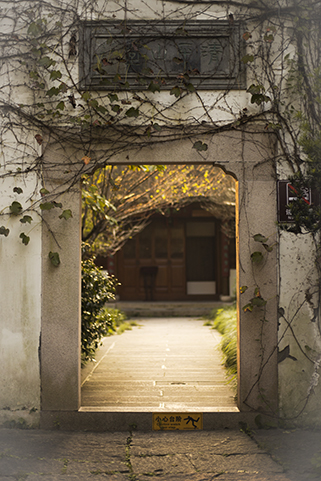
\includegraphics[width=\textwidth]{./Pictures/test.jpg} 
	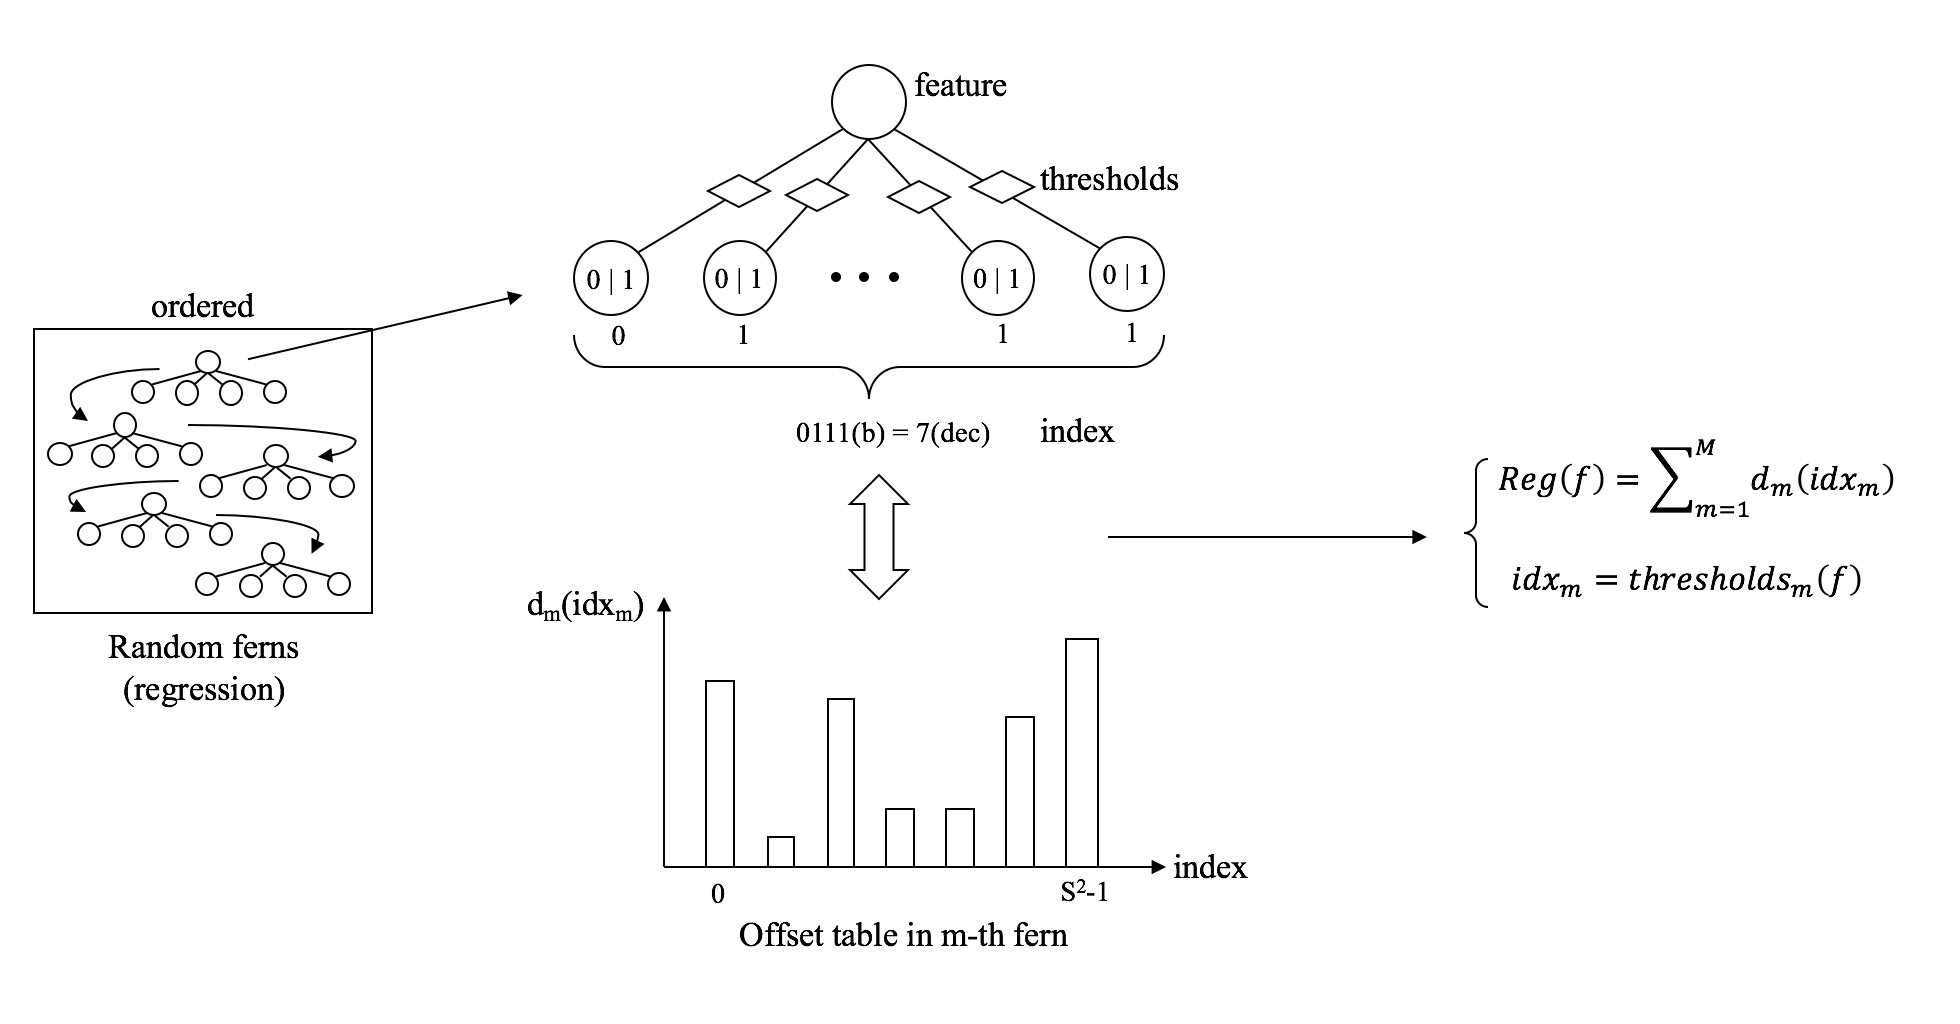
\includegraphics[width=\textwidth]{./mypic/改进后的随机蕨算法示意图.jpg} 
	\caption{改进后用于回归问题的随机蕨算法示意图} 
\end{figure}

上文表达了将随机蕨算法的核心思想,但是在实际实现该算法的时候仍将会遇到很多问题。过拟合问题是所有拟合算法中最常见的一种现象,这种现象也存在于随机蕨算法中。这一点可以通过在每一层基础蕨回归之后对每一层的回归量设置一个回归率,通过限制每一层的基础蕨的回归量上限可以非常好的抑制过拟合。虽然这种方法牺牲了一定的算法收敛速度,但是整体而言随机蕨回归算法仍旧有很高的计算速度。另外,在计算机代码实现过程中,随着随机蕨层数的增加,回归目标渐渐收敛,随机蕨的回归修正量会遇到浮点数的精度丢失问题。这个时候就需要利用额外记录每一层随机蕨回归目标均值作为保障。Algorithm 1 伪代码为随机蕨回归算法的整体概要。
% \newline
\newpage

\begin{algorithm}
\caption{随机蕨回归算法————训练模型 (Part I)}
\begin{algorithmic}[1]
\Require $D(data), L(label)$
\Require $S(depth), M(number\ of\ ferns), R(repeat\ times), eta(learning\ rate)$
\Ensure 随机蕨回归模型
\State 初始化:输入数据归一化等预处理;
\For{$M\ times$}
\Comment{随机蕨层数}
	\State $Loss_{min}\leftarrow MAX$
	\For{$R\ times$}
	\Comment{每层随机蕨重复随机过程次数}
		\State 随机产生S个维度与S个阈值:$dims, thresholds$
		\State $binary\ code=Compare(dims(D), thresholds)$
		\State \Comment 得到该基础蕨下所有训练样本的分类索引值
		\State 计算所有类内均值:$means$
		\State 更新所有训练样本的回归结果,计算$Loss$
		\If{$Loss<Loss_{min}$}
			\State 记录该基础蕨作为最佳基础蕨
% \algstore{bkbreak}
% \end{algorithmic}
% \end{algorithm}

% \begin{algorithm}
% \caption*{随机蕨回归算法————训练模型 (Part II)}
% \begin{algorithmic}[1]
% \algrestore{bkbreak}
			\State 保存该基础蕨的随机过程结果以及该随机过程下的训练样本分类均值
		\Else 
			\State $continue$
		\EndIf
	\EndFor
	\State $Y_{new}=Y_{original}-\sum_{i=0}^{m-1} Y_{pred_i}\cdot eta$
	\State \Comment 使用本次训练得到的最佳基础蕨的回归结果结合学习率更新回归目标
\EndFor
	% \State hh
\end{algorithmic}
\end{algorithm}


\begin{algorithm}
\caption{随机蕨回归算法————应用模型}
\begin{algorithmic}[1]
\Require $D(data)$,随机蕨回归模型
\Ensure $L(label)$
\State $Reg\leftarrow 0$
\Comment 初始化回归值
\For{$M\ times$}
\Comment{随机蕨层数}
	\State $binary\ code_m=Compare(dims_m(D), thresholds_m)$
	\Comment 得到本层基础随机蕨分类索引
	\State $reg_m=Indexing_m(binary\ code_m)$
	\Comment 得到本层基础随机蕨的回归值
	\State $Reg=Reg+reg_m$
	\Comment 将本次回归值累计到总回归值中去
\EndFor
\State \Return $Reg$
\end{algorithmic}
\end{algorithm}


% \newpage
% \pagebreak

\section{大噪声干扰下的随机蕨回归算法}

上一节中介绍了最基本的随机蕨回归模型,该模型在通常情况下都具有非常好的拟合能力,对于各种线性或者非线形问题都有很强的适应性。并且随机蕨回归算法在学习率的影响下,有非常好的抗过拟合能力,对轻微噪声也有很好的适应性。但是在实际应用过程中,会遇到一些数据极其不完备的情况。例如在一些回归问题中,输入的样本维度具有一定的不确定性,又或者在某些情况下输入样本的维度是一定的,但是有些维度的数据会存在严重噪声,如图2-3所示。

\begin{figure}[htb]
	\centering 
	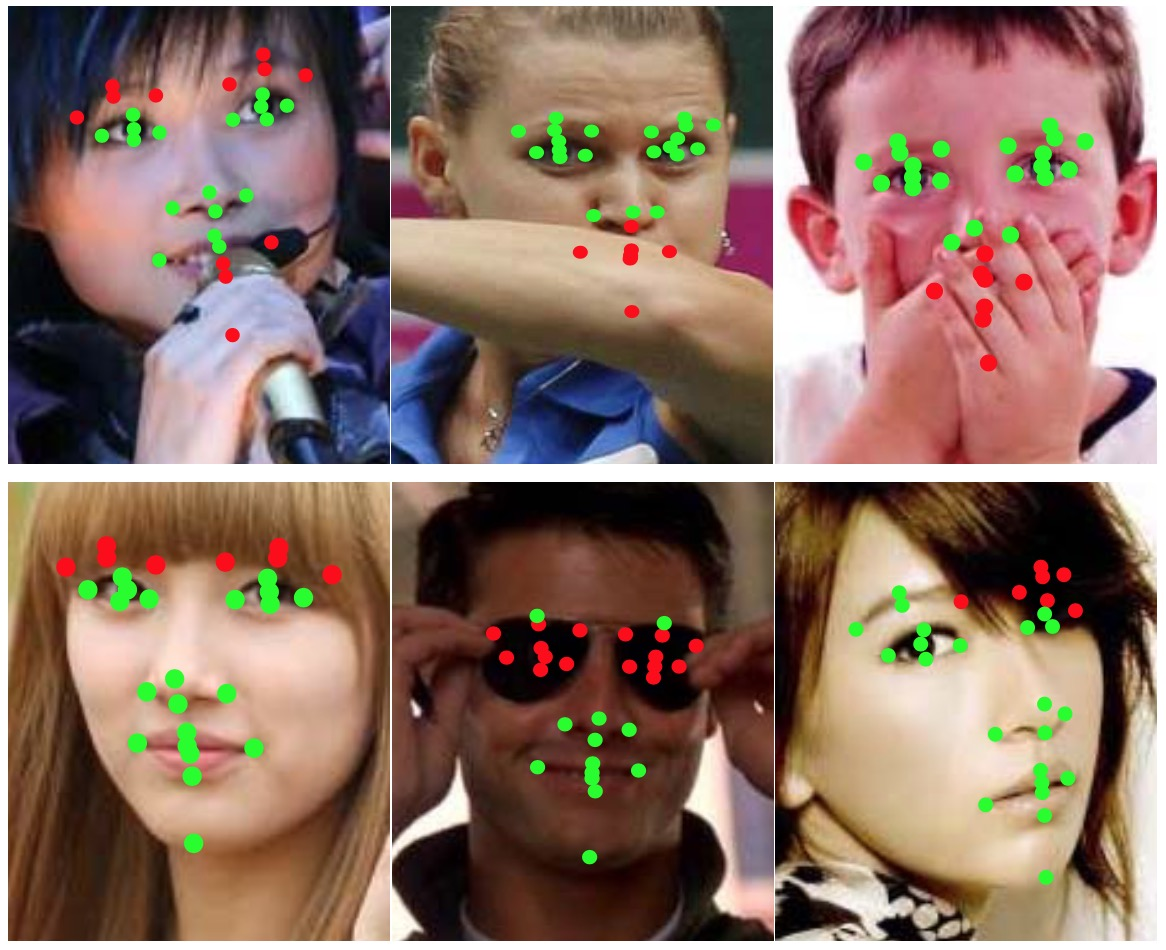
\includegraphics[width=0.7\textwidth]{./mypic/人脸特征由于被遮挡导致的缺失.jpg} 
	% 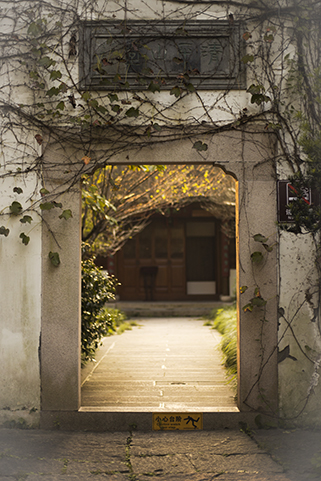
\includegraphics[scale=1.0]{./Pictures/test.jpg} 
	\caption{人脸特征(红点处)由于被障碍物遮挡导致缺失,缺失处的特征丧失了全部信息。} 
\end{figure}

这些情况下,在实验中会发现上节所述的随机蕨回归算法会遇到一个拟合能力严重不足的问题。例如存在一个输入样本特征描述$F=\{f_1,f_2,...,f_N\}$,其中有部分特征被噪声严重干扰,或者数据缺失,此时$F$为:
\begin{equation}
F=\{f_1,f_2,...f_p,f’_{p+1},...,f’_N\}
\end{equation}
其中$p+1$到$N$维特征为被噪声严重干扰的部分。这里注意随机蕨回归算法由于在选择特征维度的过程是完全随机的,不同样本也会有不同的被污染维度。例如在某一个样本中,前10个维度的特征被污染了,但是在另一个样本中后10个维度的特征被污染了,又或者在其他样本中完全随机的某些维度被污染。由于随机蕨算法中,每个基础蕨进行比较的那些维度($dims$)是完全随机生成的,因此为了方便后文阐述,上式中对于某一个样本,可以将被噪声严重污染的维度置于公式后方。

当特征存在上述被干扰情况的时候,从随机蕨算法中可以很容易看出,随机蕨算法存在两个缺陷。第一是当训练数据被干扰时,随机蕨回归模型在训练的过程中会尽量避免这些被污染的特征维度。因为一旦在随机过程中这些特征被选中,被污染的数据将会有错误的分类,并在最后分类均值的计算中严重干扰最后结果,最终导致整个随机蕨回归能力大大下降。第二是当随机蕨回归模型在训练的过程中并没有遇到严重的特征干扰问题,但是在实际应用过程中特征被大量污染以及干扰,这个时候被污染的特征维度直接导致样本的分类结果出现严重的偏差,就会导致最后的回归结果出现完全不在预期内的错误结果。

假设特征的被污染情况是可以被预测的(事实上在很多情况下这个假设是成立的,并且可以被很精确的估计),那么可以存在如下表达:
\begin{equation}
	B=\{b_1,b_2,...b_p,b_{p+1},...,b_N\}\in[0,1]
\end{equation}
其中$B$和$F$具有完全一致的维度,表示$F$的各个维度的置信度,也就是当$F$中某一维度的特征$F_i$被污染了的时候,对应的$B_i$将从百分之百可信度变为零(从1到0)。式(2-11)中假定第$1$到第$p$维都是未被污染的维度,第$p+1$到第$N$维都是被污染的维度,则有:
\begin{equation}
b_i=
\begin{cases}
1\quad {0\leq i\leq p} \\
0\quad {p<i\leq N}
\end{cases}
\end{equation}
$B$可以称为特征$F$的可信度掩码。在这个假设成立的情况下,我们可以充分利用这个信息来调整随机蕨回归算法。由于随机蕨算法中的每一个基础蕨都会根据出入特征的某几个维度进行回归,每个基础蕨在进行实际的回归之前可以先进行判断。如果该基础随机蕨要参考的那几个特征维度的可信度掩码值较低,则需要对这个随机蕨的回归量进行抑制,而当基础随机蕨参考的特征维度的可信度掩码值较高的时候,则对这个基础蕨的回归量不做调整。在算法实现过程中,特征维度的可信度掩码可以作为每个随机蕨的权值添加进算法中,也就是每个基础蕨的回归量应有如下表达:
\begin{equation}
	Reg_{fern}^{new} = Reg_{fern}^{original}\cdot f(B)
\end{equation}
其中$f(B)$为由可信度掩码生成的权值函数。在简单应用中,$f(B)$可以有简单的表达:
\begin{equation}
\begin{aligned}
	Q(i)=
	\begin{cases}
		1\quad i\in dims \\
		0\quad i\not\in dims
	\end{cases} \\
	f(B)=\frac{\sum_{i\in dims} b_i}{\sum_{i=0}^{N} Q(i)}
\end{aligned}
\end{equation}
在有了权值调整之后,当某一个基础蕨进行特征维度和阈值的比较时,会同时对可信度掩码进行处理。一旦输入的样本特征有较低的可行度时,$f(B)$将得到一个较低的值,从而抑制住这个基础蕨的回归量,避免杂乱的回归量对最后结果有较大的影响。并且这样处理仍然能让所有的维度都得到均匀的训练,不然被污染的维度会由于训练时$Loss$下降过少而被训练器忽略。同时在回归应用的时候,被污染的特征维度也会被抑制,保证最后回归结果不会因为某几个特征维度的干扰而破坏。

Algorithm 3 为增加掩码了机制的随机蕨算法的伪代码。
% \newline

\begin{algorithm}
\caption{掩码机制下的随机蕨回归算法————训练模型}
\begin{algorithmic}[1]
\Require $D(data), L(label), B(belief\ mask)$
\Require $S(depth), M(number\ of\ ferns), R(repeat\ times), eta(learning\ rate)$
\Ensure 随机蕨回归模型
\State 初始化:输入数据归一化等预处理;
\For{$M\ times$}
\Comment{随机蕨层数}
	\State $Loss_{min}\leftarrow MAX$
	\For{$R\ times$}
	\Comment{每层随机蕨重复随机过程次数}
		\State 随机产生S个维度与S个阈值:$dims, thresholds$
		\State $binary\ code=Compare(dims(D), thresholds)$
		\State \Comment 得到该基础蕨下所有训练样本的分类索引值
		\State $f(B)=\frac{\sum_{i\in dims} b_i}{\sum_{i=0}^{N} Q(i)}$
		\State \Comment 根据该基础蕨所选特征的置信度计算该基础蕨的回归量权值
		\State 计算所有类内均值:$means$
		\State $Y_{pred_i}=means(binary\ code)$
		\State $Y_{new}=Y_{original}-f(B)\cdot \sum_{i=0}^{m-1} Y_{pred_i}\cdot eta$
		\State \Comment 使用本次训练得到的基础蕨的回归结果结合学习率以及权值更新回归目标
		\State $Loss=\sum_i{\|Y_{new,i}-\overline{L_i}\|}$
		\State \Comment 计算$Loss$
		\If{$Loss<Loss_{min}$}
			\State 记录该基础蕨作为最佳基础蕨
			\State 保存该基础蕨的随机过程结果以及该随机过程下的训练样本分类均值
		\Else 
			\State $continue$
		\EndIf
	\State $\hat{Y}_{new}=\hat{Y}_{original}-\hat{f}(B)\cdot \sum_{i=0}^{m-1} \hat{Y}_{pred_i}\cdot eta$
	\State \Comment 使用最佳基础蕨的回归结果结合学习率以及权值更新回归目标
	\EndFor
\EndFor
\end{algorithmic}
\end{algorithm}

\begin{algorithm}
\caption{掩码机制下的随机蕨回归算法————应用模型}
\begin{algorithmic}[1]
\Require $D(data), B(belief\ mask)$,随机蕨回归模型
\Ensure $L(label)$
\State $Reg\leftarrow 0$
\Comment 初始化回归值
\For{$M\ times$}
\Comment{随机蕨层数}
	\State $binary\ code_m=Compare(dims_m(D), thresholds_m)$
	\Comment 得到本层基础随机蕨分类索引
	\State $reg_m=Indexing_m(binary\ code_m)$
	\Comment 得到本层基础随机蕨的回归值
	\State $Reg=Reg+reg_m$
	\Comment 将本次回归值累计到总回归值中去
\EndFor
\State \Return $Reg$
\end{algorithmic}
\end{algorithm}


\newpage

\section{实验结果与分析} % 人脸回归可以在这里写

为了验证随机蕨算法从分类问题下改进到回归问题下的合理性,本文进行了两个步骤的验证实验。首先通过一个基础拟合问题验证其基本的拟合能力,特别是对于非线性问题的拟合能力。然后在将其应用到人脸特征点定位这个高纬度、非线性的实际问题中,进一步验证其回归能力的鲁棒性。

% \subsection{对随机蕨拟合能力的验证} %

首先验证随机蕨回归算法对于非线形问题的拟合能力,本文通过构造几个非线性函数,并添加随机噪声作为测试数据进行检验。

非线性函数具有如下表达式:
\begin{equation}
	f(x) = \cos(\lambda_1\pi x)+ \lambda_2 (x+1)^2 + \lambda_3 log(x+1) + \lambda_4
\end{equation}
其中包含三角函数项、多项式函数项、以及指数性质项,每给定任意的一组$\lambda_i$参数就可以得到一个特定的非线性函数。为了定量衡量算法回归能力,本文基于上述非线性函数,在自变量区间为$[0,1]$之间随机采样500个点,同时为函数值附加方差为$\sigma^2$的高斯噪声作为拟合模型的训练数据。最后将得到的拟合模型与原始函数进行比对,在同样自变量区间取1000个采样点,计算其与真值的方差$\hat{\sigma}^2$,以方差减少量作为拟合效果的评价指标。

表格2-1给出了其中20次随机实验的结果。实验中用于随机蕨拟合回归的训练参数为:学习率$eta=0.02$,$S=4$,$M=150$,$R=20$。从实验结果可以看出,原本存在较大方差噪声的数据经过随机蕨拟合回归之后,与原始模型相比方差减少幅度均值在95\%左右,对于非线性问题具有非常好的拟合能力。

图2-4给出了一些可视化数据。图中蓝色点表示用于训练随机蕨回归模型的训练数据点,红色点为随机蕨回归模型训练好之后预测的原始函数,绿色点表示原始函数真值。可以看到,图中红色点与绿色点已经非常接近,表明了随机蕨算法的拟合能力得到了验证。

\begin{table}[htb]
	\zihao{5}
	\caption{随机蕨拟合能力检验结果表} 
	% \label{Tabkeyword}
	\centering 
	\begin{tabular}[t]{
		% |c|l|r|p{4cm}|} 
		ccccccc} 
		\toprule
		$\lambda_1$ & $\lambda_2$ & $\lambda_3$ & $\lambda_4$ & 噪声方差 & 拟合后方差 & 方差减少幅度\\ 
		\midrule
		3.37292 & 0.649499 & 0.649499 & 0.649499 & 0.5 &    0.0124&    97.5229\% \\
		3.53833 & 0.792932 & 0.792932 & 0.792932 & 0.5 &    0.0153&    96.9383\% \\
		2.99967 & -0.525472 & -0.525472 & -0.525472 & 0.5 &    0.0119&    97.6265\% \\
		2.575 & 1.9678 & 1.9678 & 1.9678 & 0.5 &    0.0070&    98.6014\% \\
		2.15032 & 0.461065 & 0.461065 & 0.461065 & 0.5 &    0.0148&    97.0353\% \\
		3.09489 & -0.157773 & -0.157773 & -0.157773 & 0.5 &    0.0080&    98.3986\% \\
		5.09176 & 1.26823 & 1.26823 & 1.26823 & 0.5 &    0.0293 &    94.1431\% \\
		3.61479 & 1.71666 & 1.71666 & 1.71666 & 0.5 &    0.0133&    97.3352\% \\
		2.66396 & 1.1875 & 1.1875 & 1.1875 & 0.5 &    0.0102&    97.9562\% \\
		3.29159 & 1.72562 & 1.72562 & 1.72562 & 0.5 &    0.0160&    96.7915\% \\
		4.97152 & 0.308569 & 0.308569 & 0.308569 & 0.5 &    0.0430&    91.3997\% \\
		3.38681 & -1.90669 & -1.90669 & -1.90669 & 0.5 &    0.0102&    97.9517\% \\
		3.80523 & -1.54795 & -1.54795 & -1.54795 & 0.5 &    0.0108&    97.8402\% \\
		5.27595 & 0.855638 & 0.855638 & 0.855638 & 0.5 &    0.0287 &    94.2662\% \\
		2.22052 & 0.2368 & 0.2368 & 0.2368 & 0.5 &    0.0064&    98.7156\% \\
		5.79584 & -1.26993 & -1.26993 & -1.26993 & 0.5 &    0.0483&    90.3486\% \\
		2.42347 & -0.731821 & -0.731821 & -0.731821 & 0.5 &    0.0113&    97.7331\% \\
		4.42034 & 0.694184 & 0.694184 & 0.694184 & 0.5 &    0.0131&    97.3814\% \\
		4.83876 & 1.05292 & 1.05292 & 1.05292 & 0.5 &    0.0305&    93.8946\% \\
		\bottomrule
	\end{tabular}
\end{table}


\begin{figure}[htb]
	\centering 
	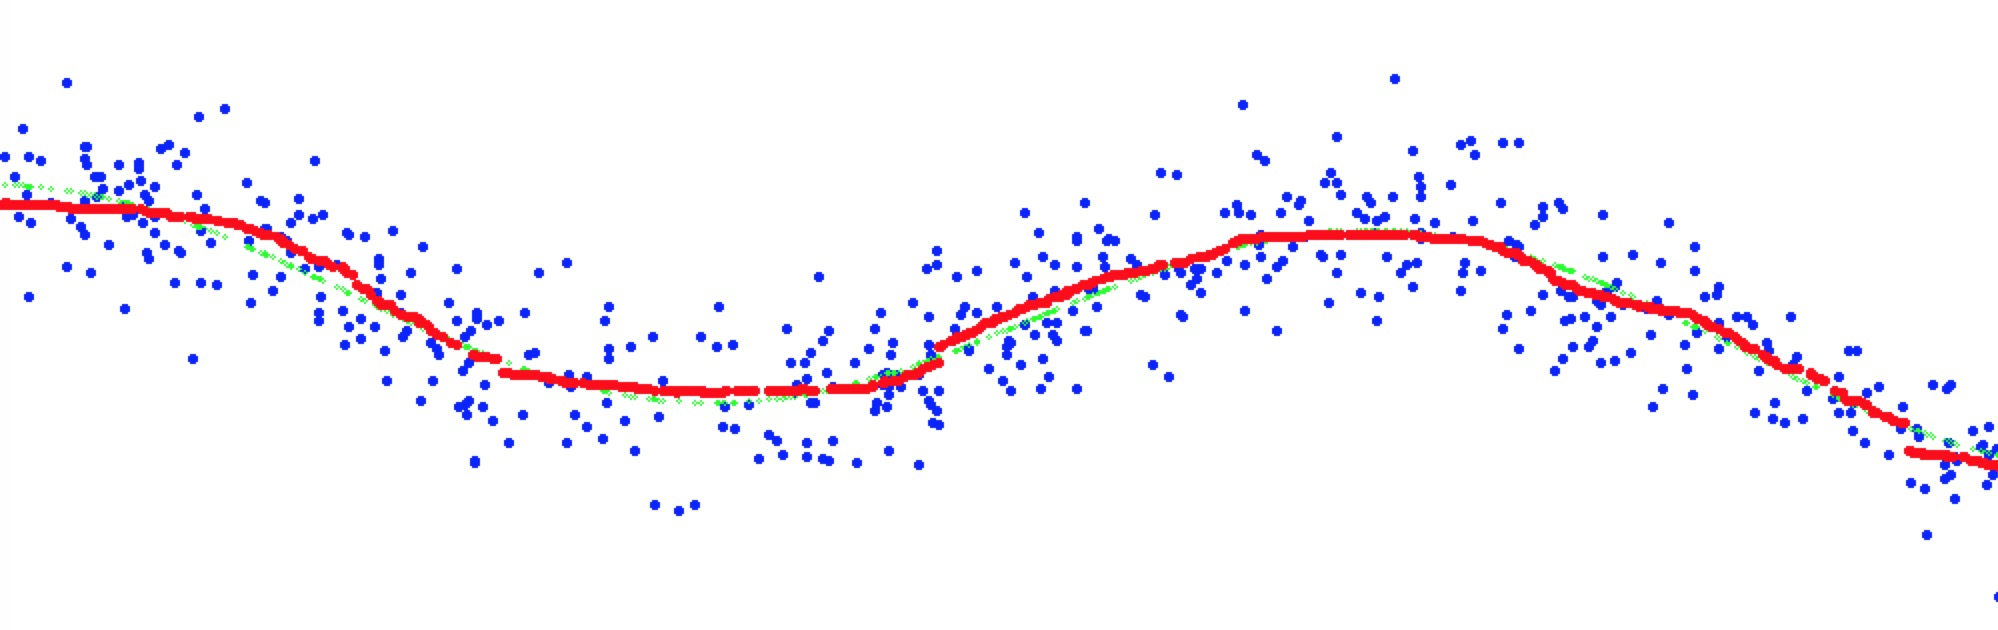
\includegraphics[width=0.6\textwidth]{./mypic/随机蕨回归实验1.jpg} 
	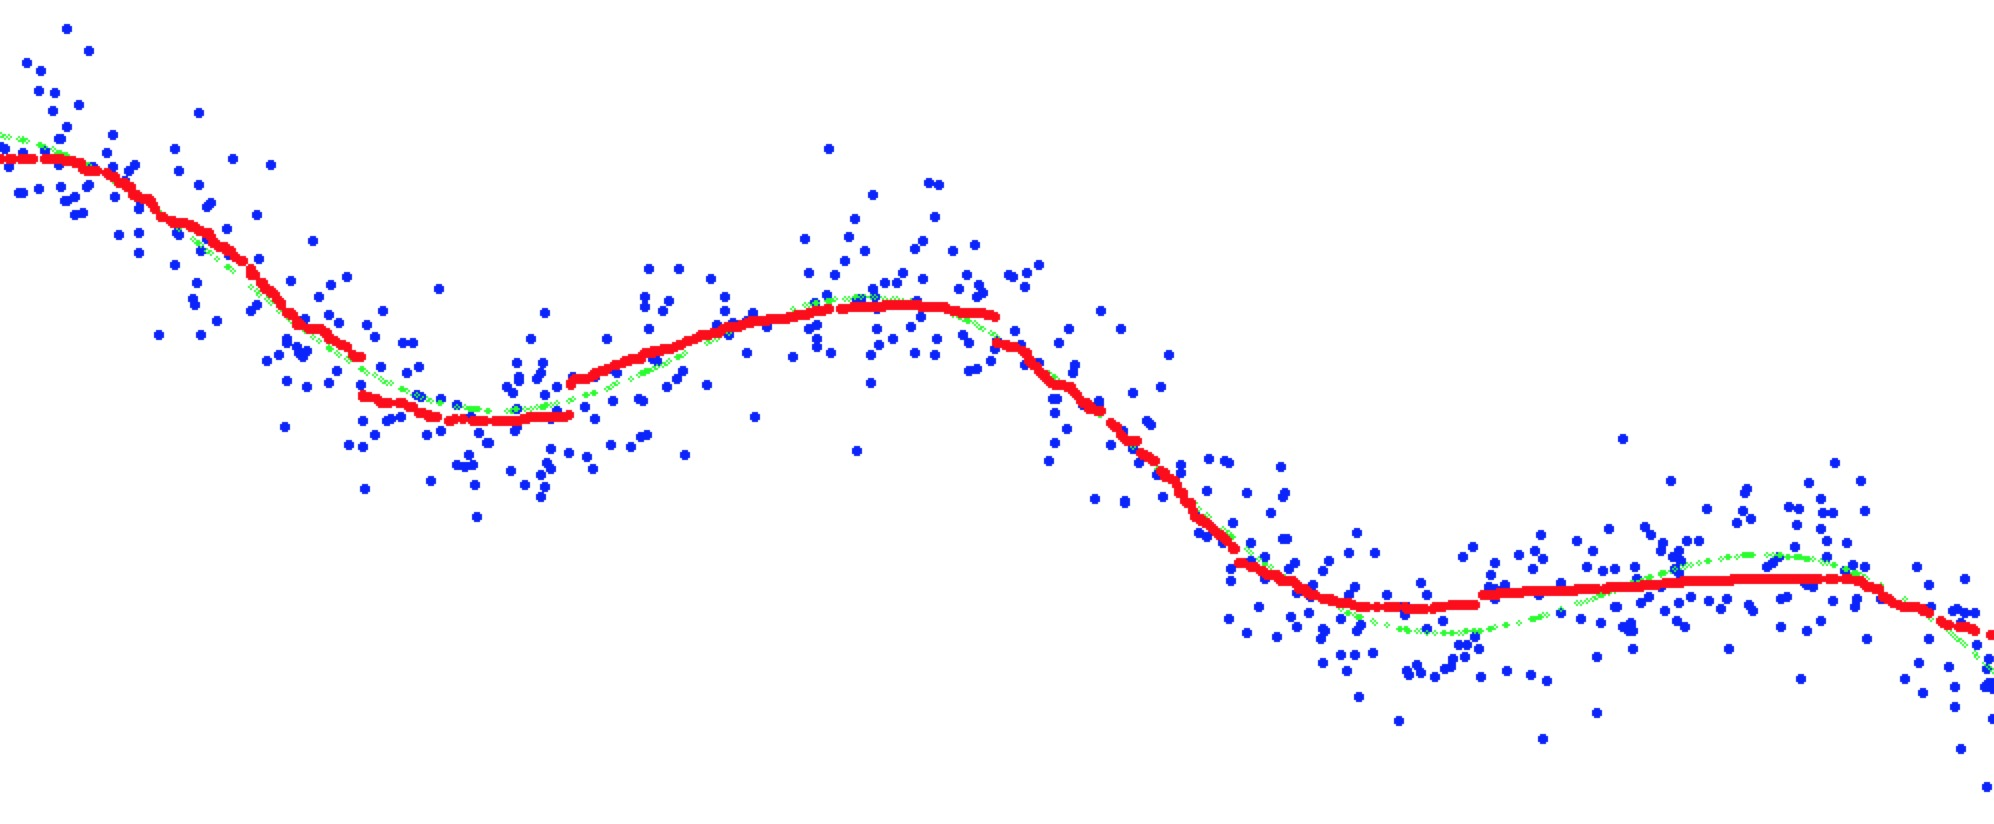
\includegraphics[width=0.6\textwidth]{./mypic/随机蕨回归实验2.jpg} 
	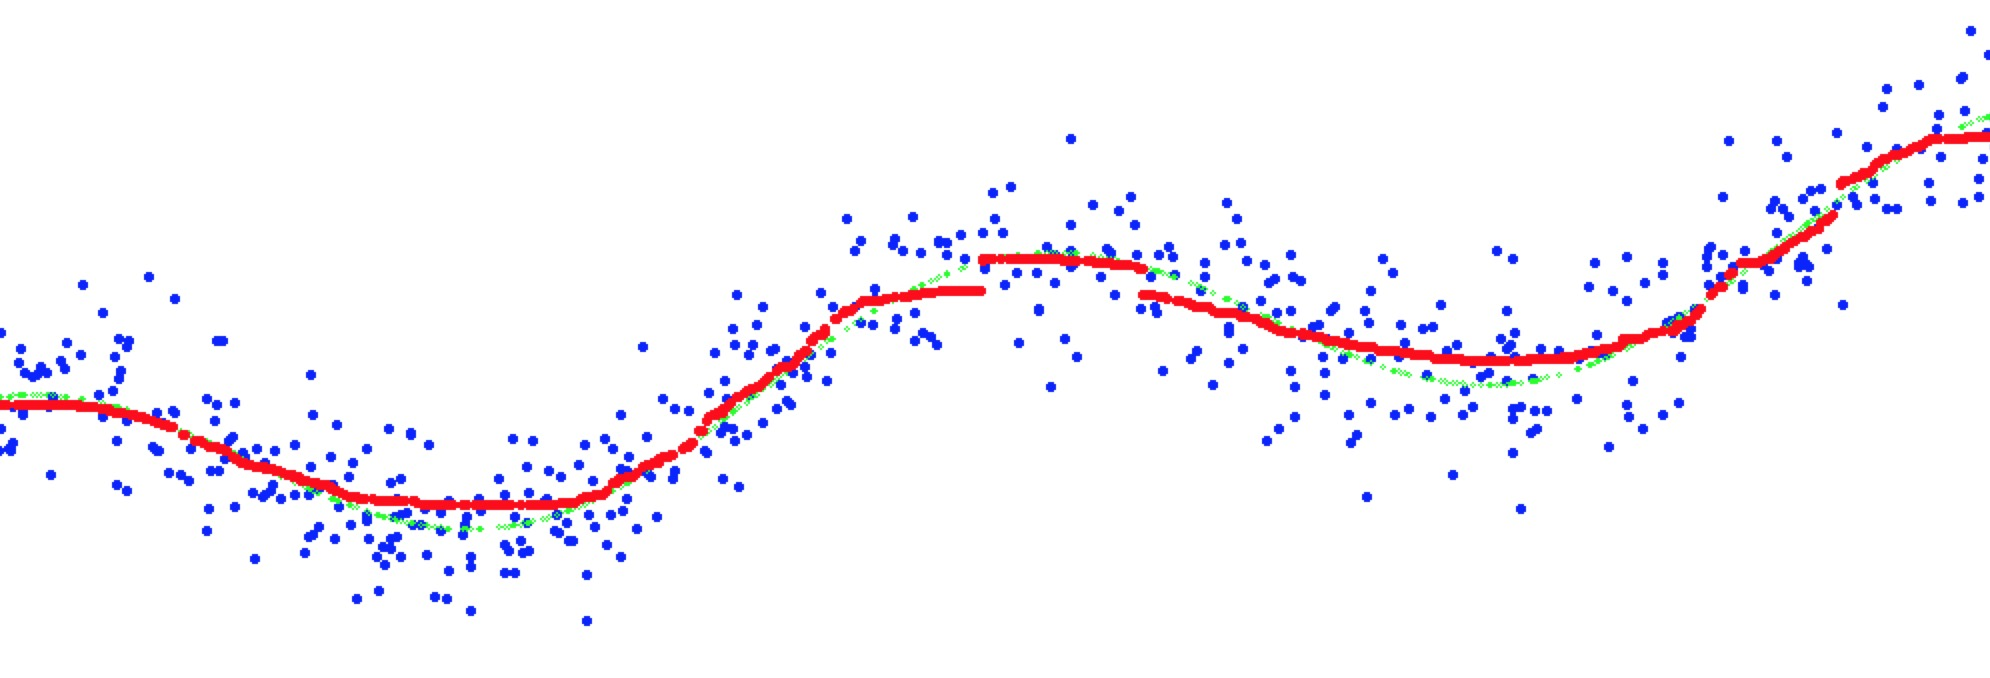
\includegraphics[width=0.6\textwidth]{./mypic/随机蕨回归实验3.jpg} 
	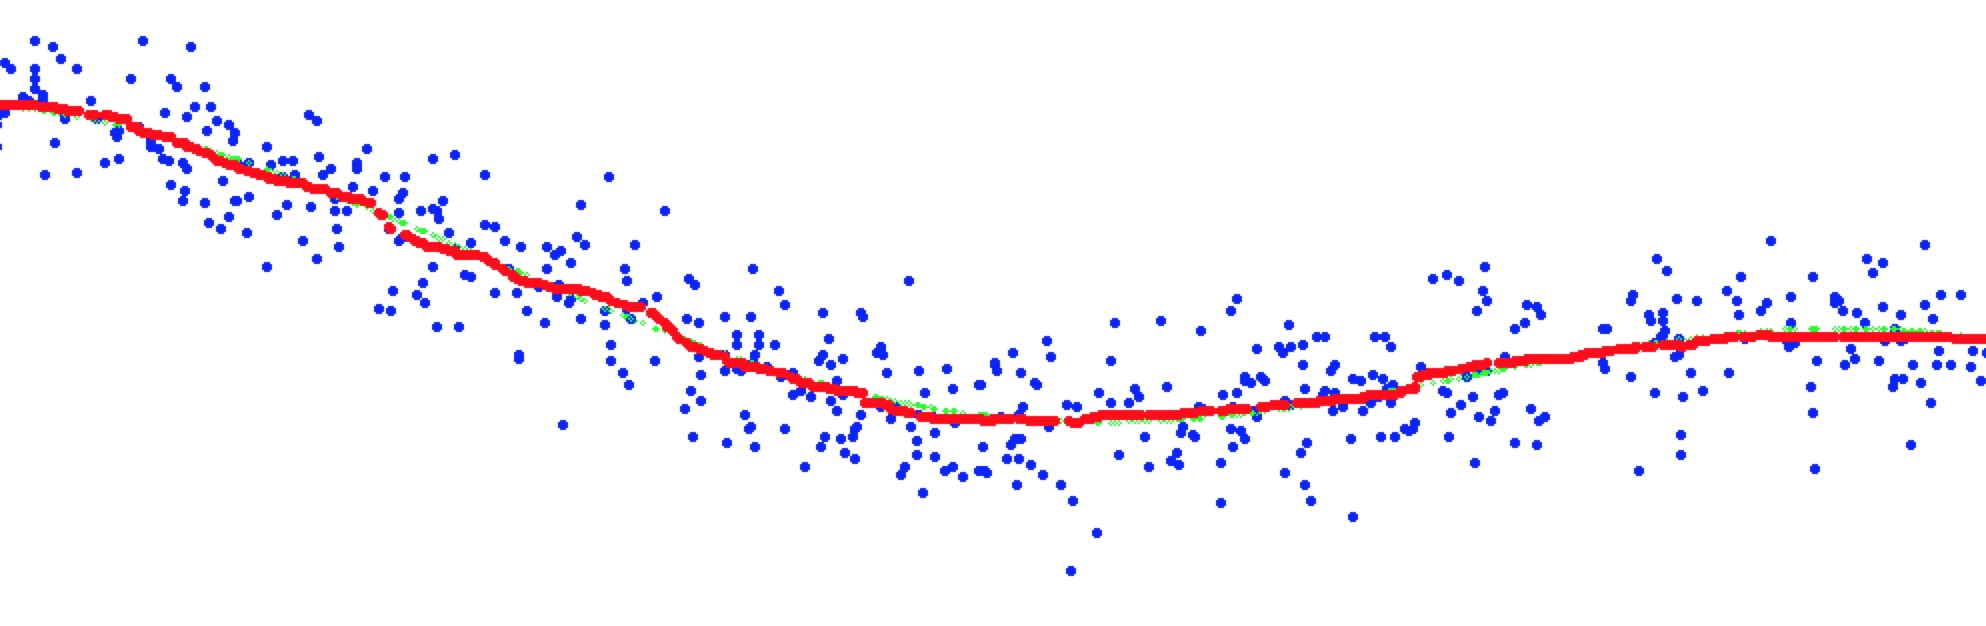
\includegraphics[width=0.6\textwidth]{./mypic/随机蕨回归实验4.jpg} 
	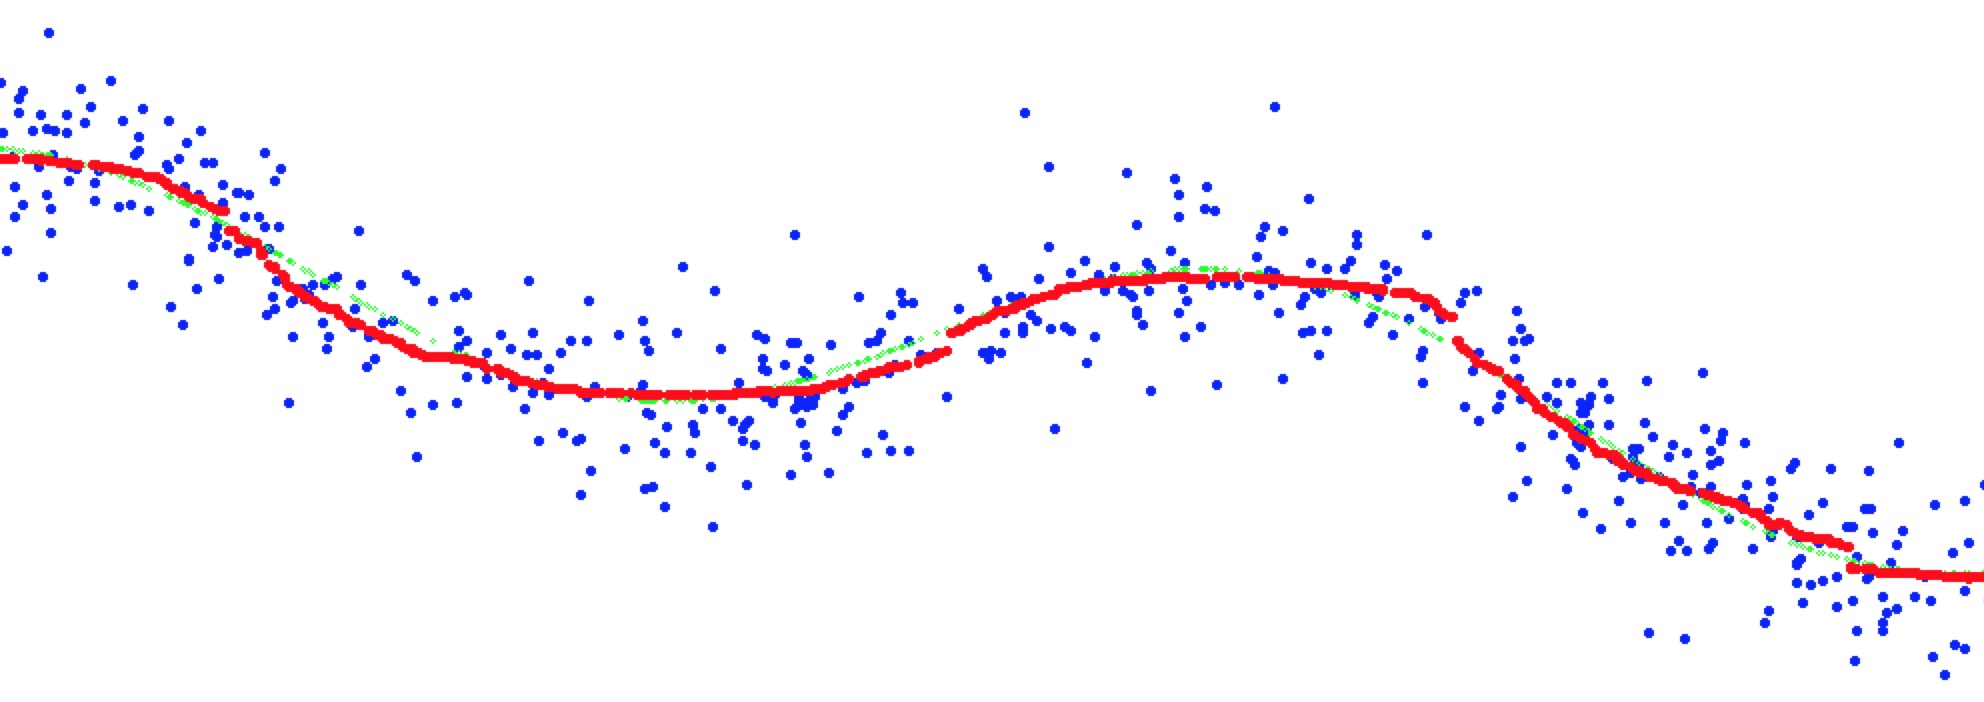
\includegraphics[width=0.6\textwidth]{./mypic/随机蕨回归实验5.jpg} 
	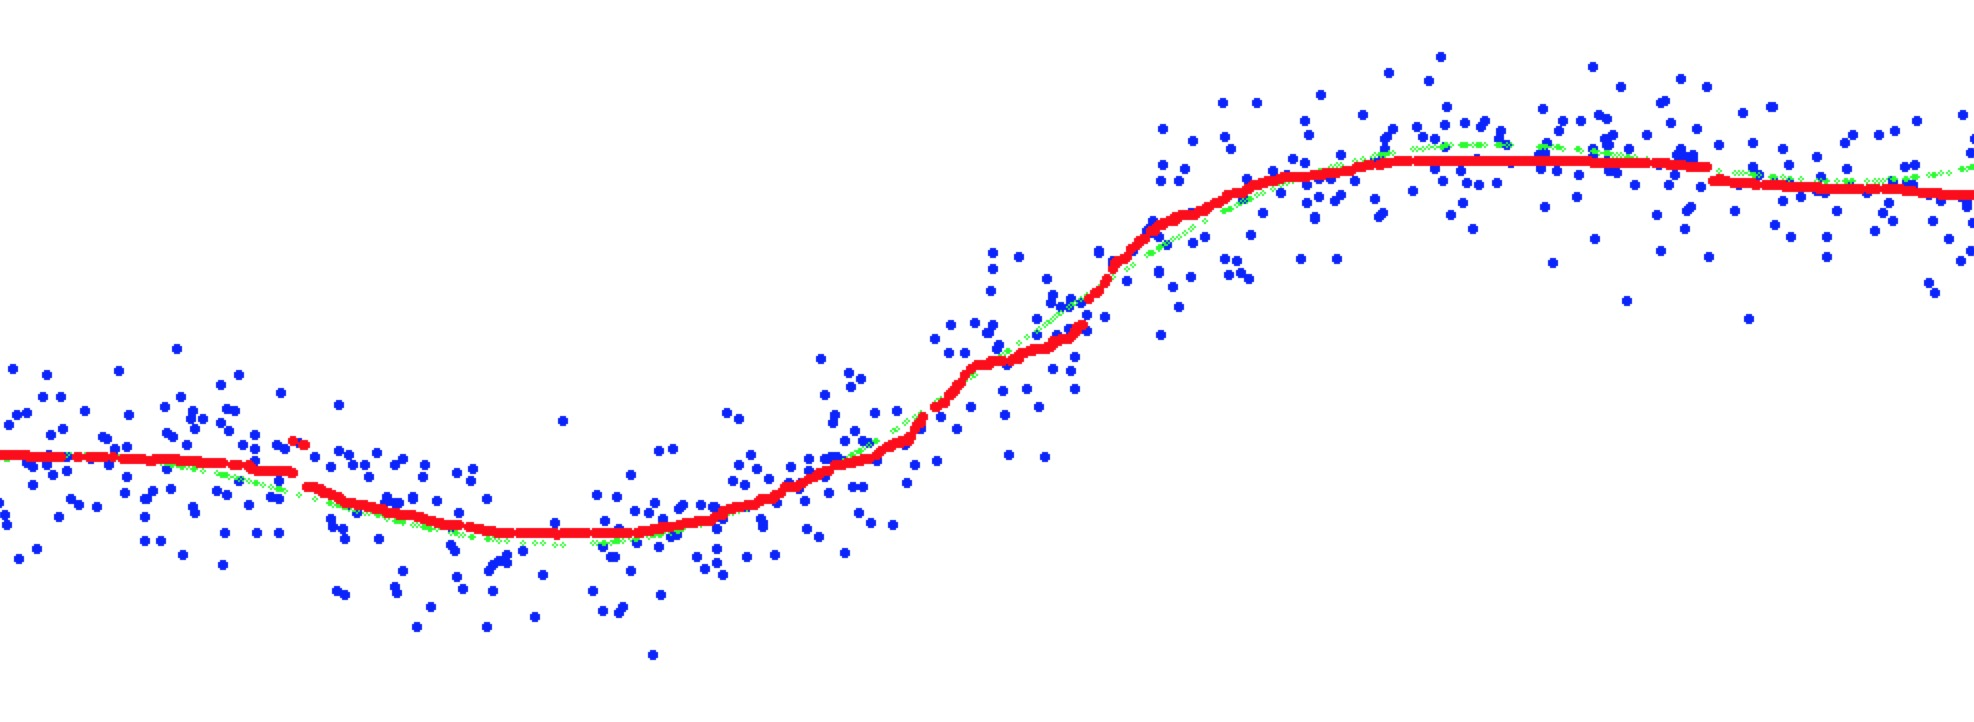
\includegraphics[width=0.6\textwidth]{./mypic/随机蕨回归实验6.jpg} 
	% 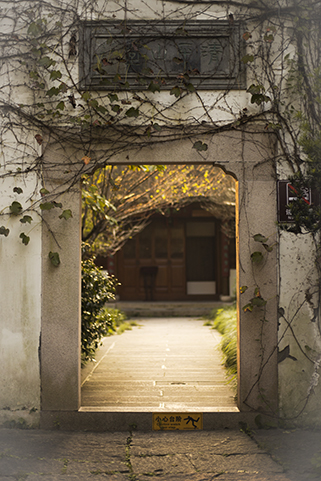
\includegraphics[scale=1.0]{./Pictures/test.jpg} 
	\caption{随机蕨回归实验可视化结果} 
\end{figure}

除此之外,本文还将该随机蕨回归算法应用到人脸特征点定位这个更为复杂的回归问题中去,同样也取得了非常不错的表现。由于该实验涉及一些与本文相关度不高的中间步骤,因此具体实验细节在此不作详述,仅给出实验最后得到的人脸特征点定位结果。图2-5中红色圆点表示通过随机蕨回归器得到的人脸特征点定位结果。该实验中涉及的随机蕨回归模型具有高达1000维度输入以及136维度的回归目标,具有极高的回归复杂度。其优良的表现再次证明了随机蕨回归算法的可行性。

并且,本文将该人脸特征点定位算法结果与现有最为优秀的几个算法进行了比较。通过在300-W数据集\cite{sagonas2013semi}上,采用瞳孔间距正则化误差作为评价标准\cite{belhumeur2013localizing}\cite{cao2014face},本文得到如表2-2所示的结果。从表2-2可以看出,本文算法相比于ESR\cite{cao2014face}、SDM\cite{xiong2013supervised}、LBF fast\cite{ren2014face}这三种算法有更小的误差(其中300-W数据集包含一般数据集和复杂数据集两个部分),并且在算法效率上仅次于LBF fast。此实验中其他三种算法的实验结果均引用于文章[\citenum{ren2014face}],对于精度对比没有影响,但本文算法的帧率测试由于实验平台不同,仅供参考(本文实验环境为2.2GHz Intel Core i7单进程处理器)。该实验可以表明,改进后的随机蕨算法不光具有较好的拟合能力,同时也具备较高的计算效率。

\begin{figure}[htb]
	\centering 
	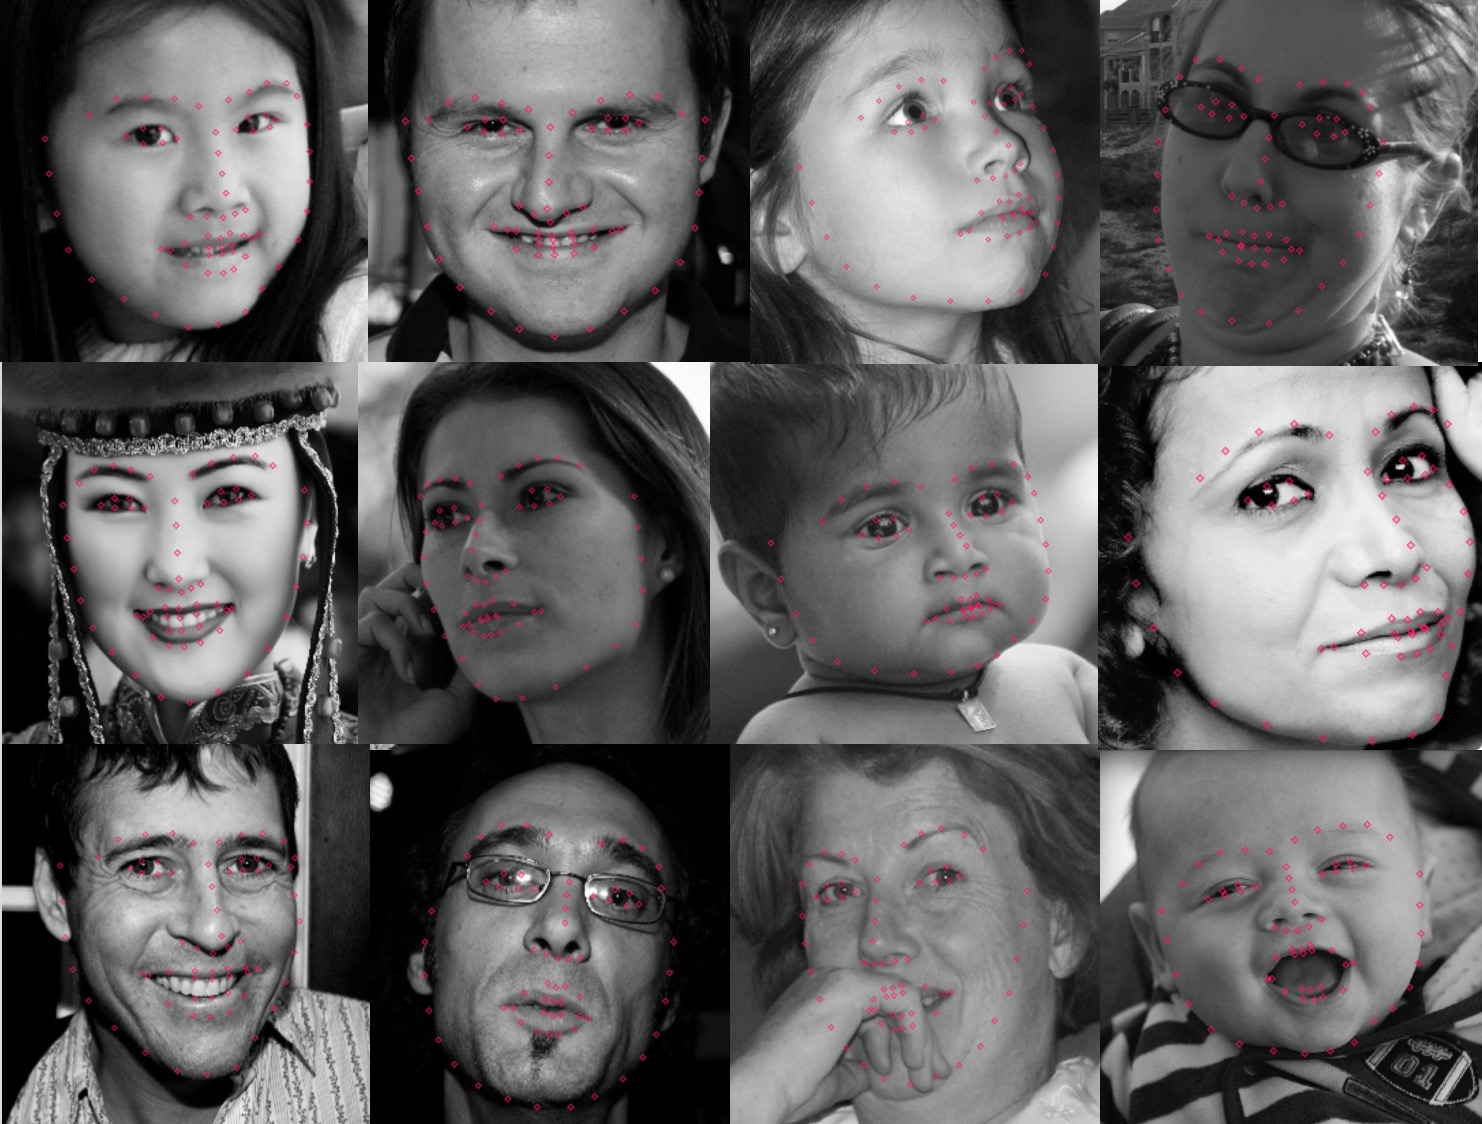
\includegraphics[width=\textwidth]{./mypic/人脸特征点定位实验.jpg} 
	% 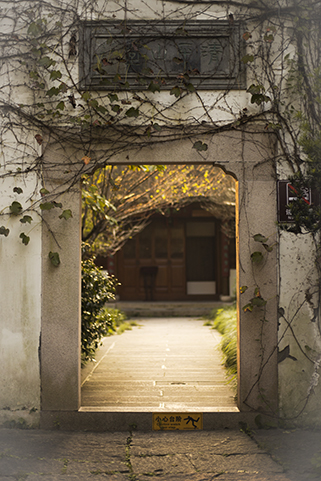
\includegraphics[scale=1.0]{./Pictures/test.jpg} 
	\caption{人脸特征点定位实验结果} 
\end{figure}

\begin{table}[htb]
	\zihao{5}
	\caption{300-W数据集上人脸特征点定位算法对比} 
	% \label{Tabkeyword}
	\centering 
	\begin{tabular}[t]{
		% |c|l|r|p{4cm}|} 
		ccccccc} 
		\toprule
		算法 & 全数据集误差 & 一般数据集误差 & 复杂数据集误差 & 帧率(FPS)\\ 
		\midrule
		ESR\cite{cao2014face} & 7.58 & 5.28 & 17.00 & 120 \\
		SDM\cite{xiong2013supervised} & 7.52 & 5.6 & 15.4 & 70 \\
		LBF fast\cite{ren2014face} & 7.37 & 5.38 & 15.5 & 3100 \\
		Ours & 6.94 & 4.93 & 15.18 & 476 \\
		\bottomrule
	\end{tabular}
\end{table}


% \subsection{对大噪声干扰下的随机蕨算法验证} % 

大噪声干扰下的随机蕨算法验证实验由于与本文第四章实验有较多相互依赖的交集,因此对于该问题的实验验证将在节4.6中进行展开,此处不再详细讨论。


\section{本章小结}
本章旨在充分开发随机蕨算法的潜能,通过改造整理,先是总结出经典随机蕨算法应用于回归问题的改进方法,再进一步结合实际问题中存在大噪声干扰下随机蕨算法不够鲁棒的情况,提出掩码机制下的随机蕨回归算法。最后还通过实验验证了随机蕨算法在非线性回归问题下的拟合能力,通过人脸特征点定位这个具有非常大挑战性的回归问题,证实了本章提出的随机蕨回归算法具有较好的实用性以及高效性。
























\chapter{基于OpenGL的深度相机仿真环境搭建}

\section{概述}
大数据驱动下的模型等训练需要大量带有人工标注真值的数据作为基础。深度相机作为近几年流行起来的新型相机,能够获取除了颜色意外的额外的视觉信息,极大促进了物体位姿估计领域的研究发展。物体位姿估计领域内越累越多的基于深度相机采集的深度图像的算法被提出并取得了不错的效果。但是这些物体位姿估计算法很难应用到实际生产生活中去,有一个很大的原因在于这些算法都依赖带有真值标注等训练数据,而这些带有真值的训练数据非常难以获取。有真值标注的训练数据的可获取性和易获取程度极大的影响到了物体位姿估计算法的进一步发展,因此本章将针对这一点,讨论一个基于OpenGL平台的深度相机仿真环境。

本章的主旨在于能够通过任意指定一个刚性物体的3D数据文件,便可以借助OpenGL计算模拟深度相机,自动并且快速地给出大量带有真值标注的深度相机仿真深度数据。由于本文研究内容主要在于位姿估计方面,因此本文给出的深度相机仿真环境给出的数据主要有仿真深度图像以及给定物体在仿真相机下的6维位姿$P$。其中这6维位姿包括以相机参考系为参考系下的物体的欧几里得坐标($P_x,P_y,P_z$),以及相机参考系下的欧拉角位姿($P_ax,P_ay,P_az$),如下图所示:

\begin{figure}[htb]
	\centering 
	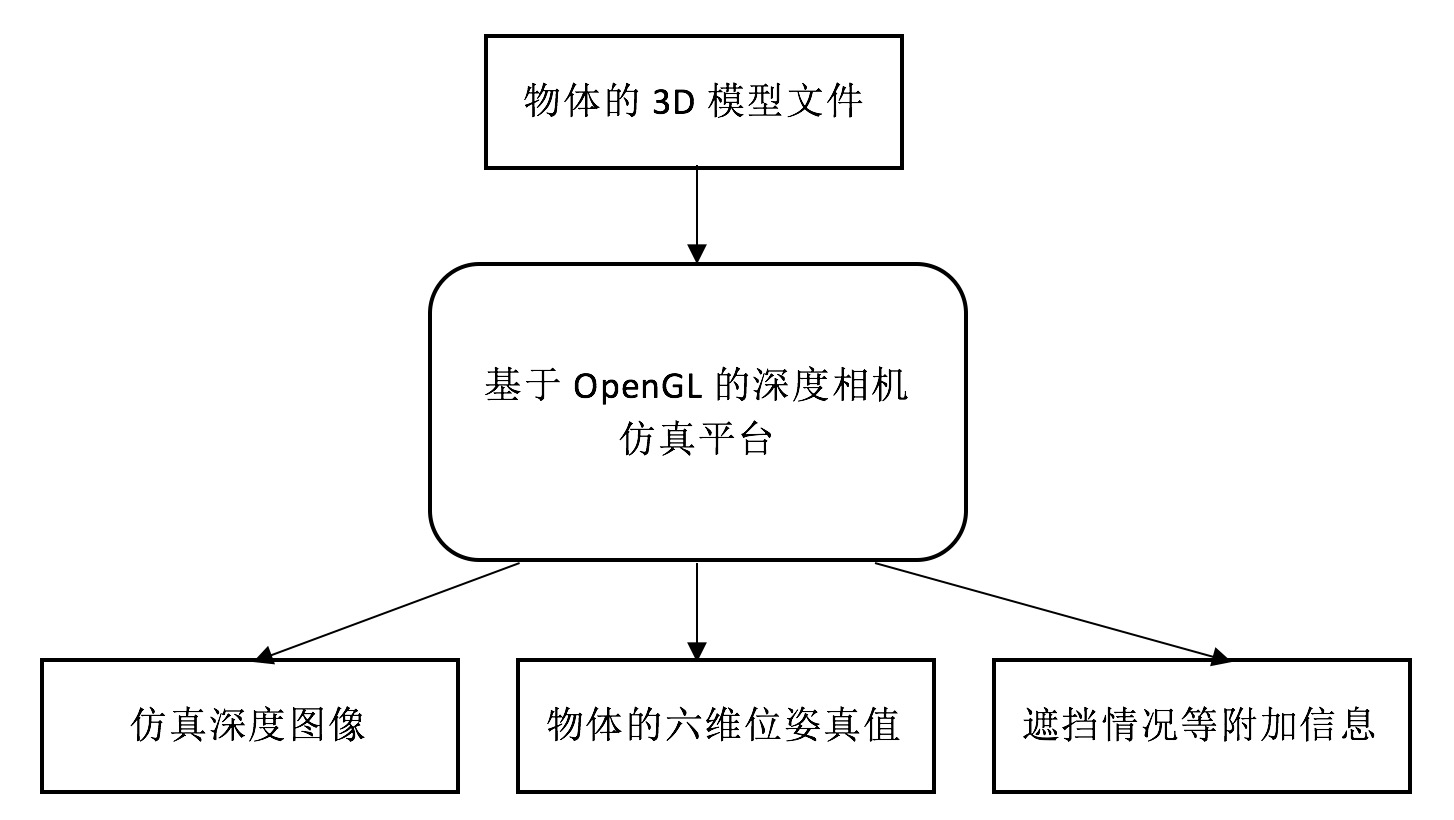
\includegraphics[width=0.7\textwidth]{./mypic/仿真深度相机系统结构.jpg} 
	% 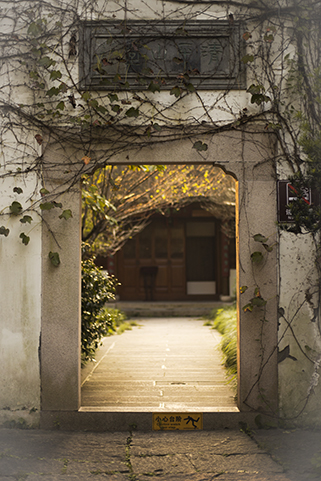
\includegraphics[scale=1.0]{./Pictures/test.jpg} 
	\caption{仿真深度相机系统架构示意图} 
\end{figure}

本章结构安排如下:3.2节主要介绍仿真环境中的数学模型,包括几何投影变换、坐标系的定义以及OpenGL平台中需要用到的一些基本理论。3.3节将阐述仿真环境搭建的具体流程以及如何改进仿真环境得到的数据,使仿真数据更加接近真实情况。最后在3.4节中通过具体的实验结果来验证得到的仿真数据的可行性。


\section{仿真数学模型}
% \subsection{两种几何变换}
在图像处理计算过程中,经常会遇到两种经典的变换,一种是仿射变换(Affine Transform),另一种是透视变换(Perspective Transform)。其中仿射变换是一种平面坐标系的伸缩旋转变换,是一种线形的变换,会保持原有图像的平行性,也就是说在原本图像中如果保持平行的两条直线,在经过仿射变换之后仍旧会保持平行。如图3-2所示:

\begin{figure}[htb]
	\centering 
	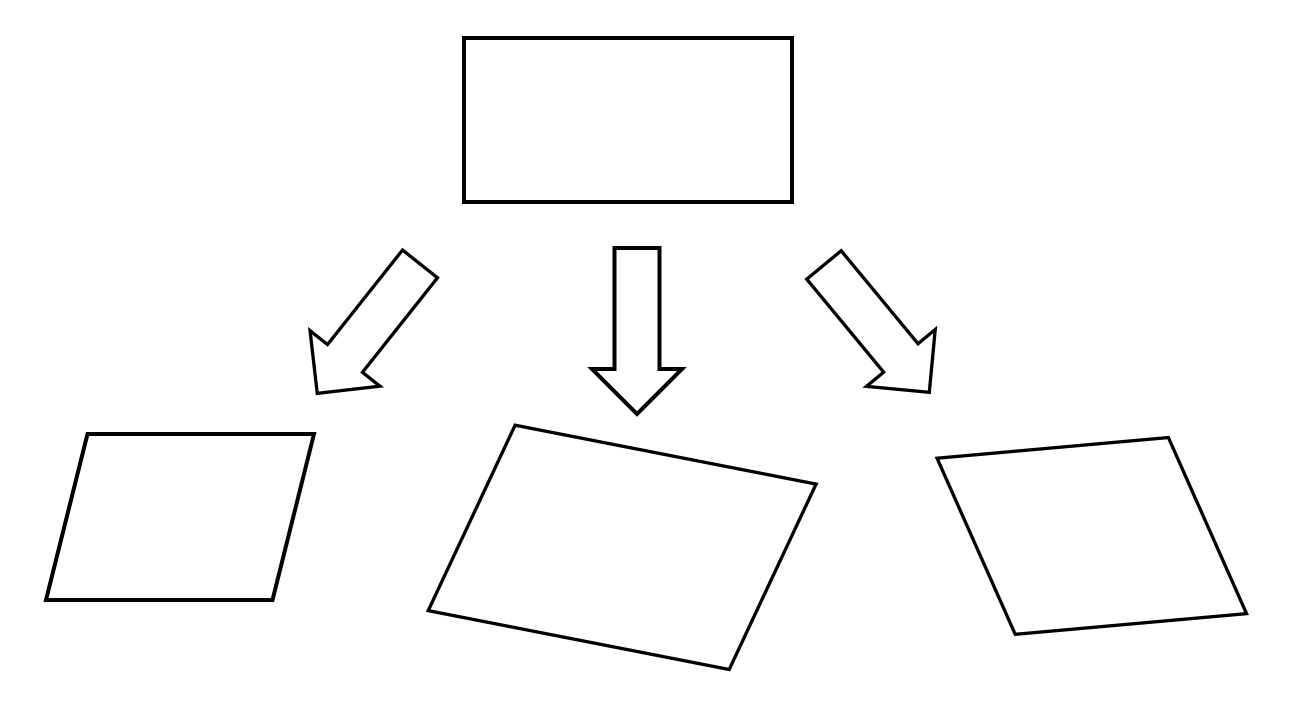
\includegraphics[width=0.7\textwidth]{./mypic/仿射变换示意图.jpg} 
	% 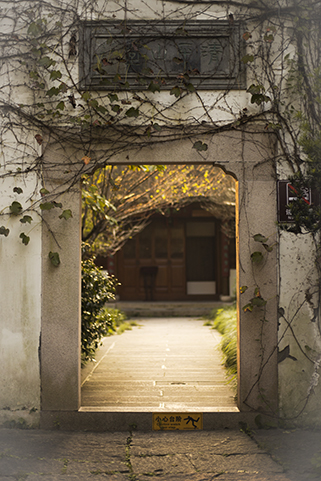
\includegraphics[scale=1.0]{./Pictures/test.jpg} 
	\caption{仿射变换示意图,平行四边形进行放射变换后仍旧是平行四边形} 
\end{figure}

仿射变换的变换可以由一个$2*3$的矩阵$Rt_{affine}$来表达:
\begin{equation}
	Rt_{affine}=\left[R\quad T\right]=
	\left[
	\begin{aligned}
	r_{11}\quad r_{12}\quad t_1 \\
	r_{21}\quad r_{22}\quad t_2
	\end{aligned}
	\right]
\end{equation}
上式中$R$表示坐标系的旋转,$T$表示坐标系的平移。在仿射变换下,若给定一个点$P:(x,y)$,其仿射变换后将得到点$P':(x',y')$如下:
\begin{equation}
	[x'\quad y']^\top=Rt_{affine}\cdot [x\quad y\quad 1]^\top=
	\left[
	\begin{aligned}
	r_{11}\quad r_{12}\quad t_1 \\
	r_{21}\quad r_{22}\quad t_2
	\end{aligned}
	\right]\cdot 
	\left[
	\begin{aligned}
	x \\
	y \\
	1
	\end{aligned}
	\right]
\end{equation}
		
透视变换则是指利用透视中心、像点、目标点三点共线的条件,按透视旋转定律使承影面(透视面)绕迹线(透视轴)旋转某一角度,破坏原有的投影光线束,仍能保持承影面上投影几何图形不变的变换。透视变换本质上是一种三维空间上的投影变换,如下图所示:
\begin{figure}[htb]
	\centering 
	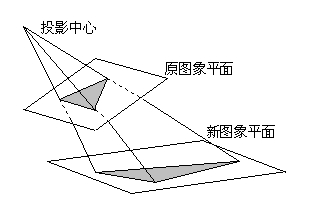
\includegraphics[scale=1.0]{./mypic/透视变换.jpg} 
	\caption{透视变换} 
\end{figure}

也就是说透视变换是将原始图像从三维空间投影到二维空间。例如给定一个初始点$P:(x,y,z)$,这个点投影到二维平面可以通过一个$3*3$的矩阵$P$表达:
\begin{equation}
	P=
	\left[
	\begin{aligned}
	a_{11}\quad a_{12}\quad a_{13} \\
	a_{21}\quad a_{22}\quad a_{23} \\
	a_{31}\quad a_{32}\quad a_{33}
	\end{aligned}
	\right]
\end{equation}
假设投影平面的坐标基表示为$(u,v)$,则有:
\begin{equation}
	\left[
	\begin{aligned}
	x \\
	y \\
	z
	\end{aligned}
	\right]=
	\left[
	\begin{aligned}
	a_{11}\quad a_{12}\quad a_{13} \\
	a_{21}\quad a_{22}\quad a_{23} \\
	a_{31}\quad a_{32}\quad a_{33}
	\end{aligned}
	\right]\cdot
	\left[
	\begin{aligned}
	u \\
	v \\
	1
	\end{aligned}
	\right]
\end{equation}
从而可以得到投影后的新坐标表达为:
\begin{equation}
\begin{aligned}
	x'=\frac{x}{z}=\frac{a_{11}u+a_{12}v+a_{13}}{a_{31}u+a_{32}v+a_{33}}
		=\frac{k_{11}u+k_{12}v+k_{13}}{k_{31}u+k_{32}v+1} \\
	y'=\frac{y}{z}=\frac{a_{21}u+a_{22}v+a_{23}}{a_{31}u+a_{32}v+a_{33}}
		=\frac{k_{21}u+k_{22}v+k_{23}}{k_{31}u+k_{32}v+1}
\end{aligned}
\end{equation}

对比上面两种变换方式可以看出,一个仿射变换最多需要有6个参数来确定,而一个投影变换的最多参数量达到了8个。投影变换相比仿射变换具有更高的复杂度,因此从模型简易角度来讲,利用仿射变换进行深度相机的仿真环境搭建更为简洁方便。一些点线扫描式的深度采集设备也是符合仿射变换模型进行深度图像采集的。

然而现实生活中,更多数量的深度相机原理大致可以分为两类,一种是基于结构光的,另一种是基于ToF(Time of Flight)的。基于结构光的深度相机通过发射结构光,并利用另一个相机采集到的视差信息构建深度图像。基于ToF的深度相机则是通过一个红外线激光发射器发射出红外线,再通过另一个红外线接收装置采集红外线照射到物体之后返回的时间,通过这个时间差来计算物体到达相机的距离。在这两种深度相机模型下,深度相机都可以被近似看作一个质点,也就是这些真实的深度相机都是以相机作为投影点,将物体深度信息投影到像平面上的到的深度图像。这一模型符合投影变换的框架,因此本文的仿真深度环境搭建也是基于投影变换进行搭建的。

下图为本文的仿真环境的一个简单几何说明图:
\begin{figure}[htb]
	\centering 
	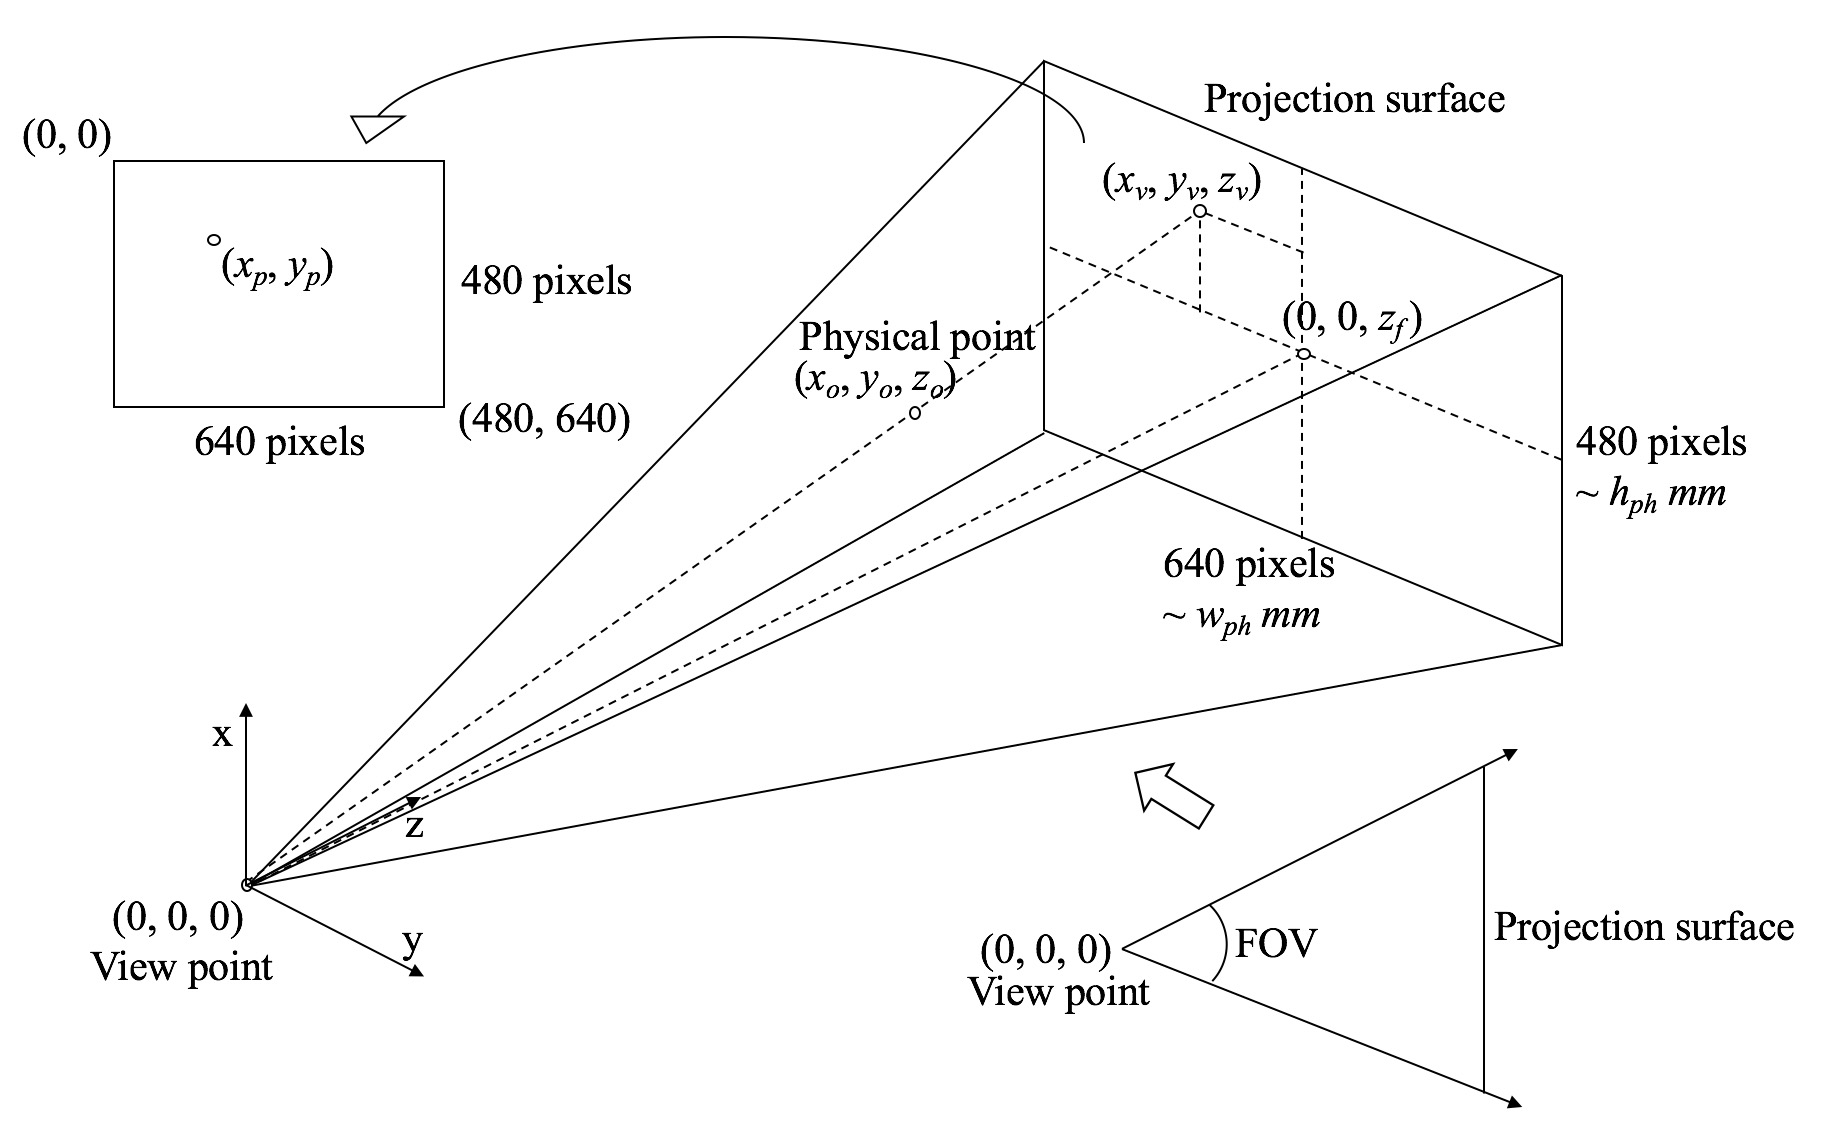
\includegraphics[width=\textwidth]{./mypic/projection.jpg} 
	\caption{仿真环境几何示例} 
\end{figure}

其中定义仿真相机位于世界坐标的原点$O$,也就是相机坐标系和世界坐标系重合。定义深度投影平面(Projection Surface)的分辨率为640*480像素。其中存在一个模拟物理点(Physical Point),记为$P_0:(x_0,y_0,z_0)$,其按照投影变换的规则将投影在投影平面上的点$P_v:(x_v,y_v,z_v)$处,并且原点$O$、模拟物理点$P_0$以及投影点$P_v$三点共线。因此存在如下等式:
\begin{equation}
	\frac{x_0}{x_v}=\frac{y_0}{y_v}=\frac{z_0}{z_v}
\end{equation}
图中涉及另外几个OpenGL的基本定义。投影平面(Projection Surface)具有事先给定的深度值$z_f$,并且垂直于相机坐标系下的$z$轴方向。像平面定义为标准VGA图像大小,也就是$640*480$分辨率大小,并且定义其横向从左往右为$x$轴方向,纵向从上往下为$y$方向。FOV(Field of View),也就是视场角。FOV定义为投影平面的上边界与下边界分别与相机坐标原点形成的角度,可以描述深度相机的视野角度。

有了上述基本定义之后,就可有如下几个等式:
\begin{equation}
\begin{aligned}
	\frac{pixels\ in\ width}{pixels\ in\ height}=
	\frac{640}{480}=
	\frac{w_{ph}}{h_{ph}} \\
	h_{ph}=2\cdot z_f \cdot \tan(FOV/2)
\end{aligned}
\end{equation}
其中$w_{ph}$和$h_{ph}$分别表示物理投影面的实际物理宽度和长度,从而对于模拟物理点$P_0:(x_0,y_0,z_0)$在深度图像中对应的像素位置关系为:
\begin{equation}
\begin{aligned}
	\frac{x_v}{h_{ph}/2}=\frac{pixels\ in\ height/2-x_p}{pixels\ in\ height/2} \\
	\frac{y_v}{w_{ph}/2}=\frac{pixels\ in\ width/2+y_p}{pixels\ in\ width/2}
\end{aligned}
\end{equation}
联立上述几个式子可以解得:
\begin{equation}
\begin{aligned}
	x_p=\left(1-\frac{x_0}{z_0\cdot\tan(FOV/2)}\right)\cdot \frac{pixels\ in\ height}{2} \\
	y_p=\left(\frac{y_0}{z_0\cdot\tan(FOV/2)}-1\right)\cdot \frac{pixels\ in\ width}{2}
\end{aligned}
\end{equation}

从上式可以看出,只要指定好FOV角度大小以及确定深度图像的分辨率大小,任意空间坐标$P_0:(x_0,y_0,z_0)$都可以直接计算的到投影变换下的像平面像素位置。

% \subsection{坐标系以及坐标系转换} % 四元数、参考系的转换等
% 深度相机仿真环境中,除了世界坐标系以外,每一个物体都有其本身的坐标系。在OpenGL环境中,我们将假想的深度相机置于世界坐标原点,并将深度相机坐标系与世界坐标系完全重合,从而可以有如下图所示的一个基本几何定义:
% \begin{figure}[htb]
% 	\centering 
% 	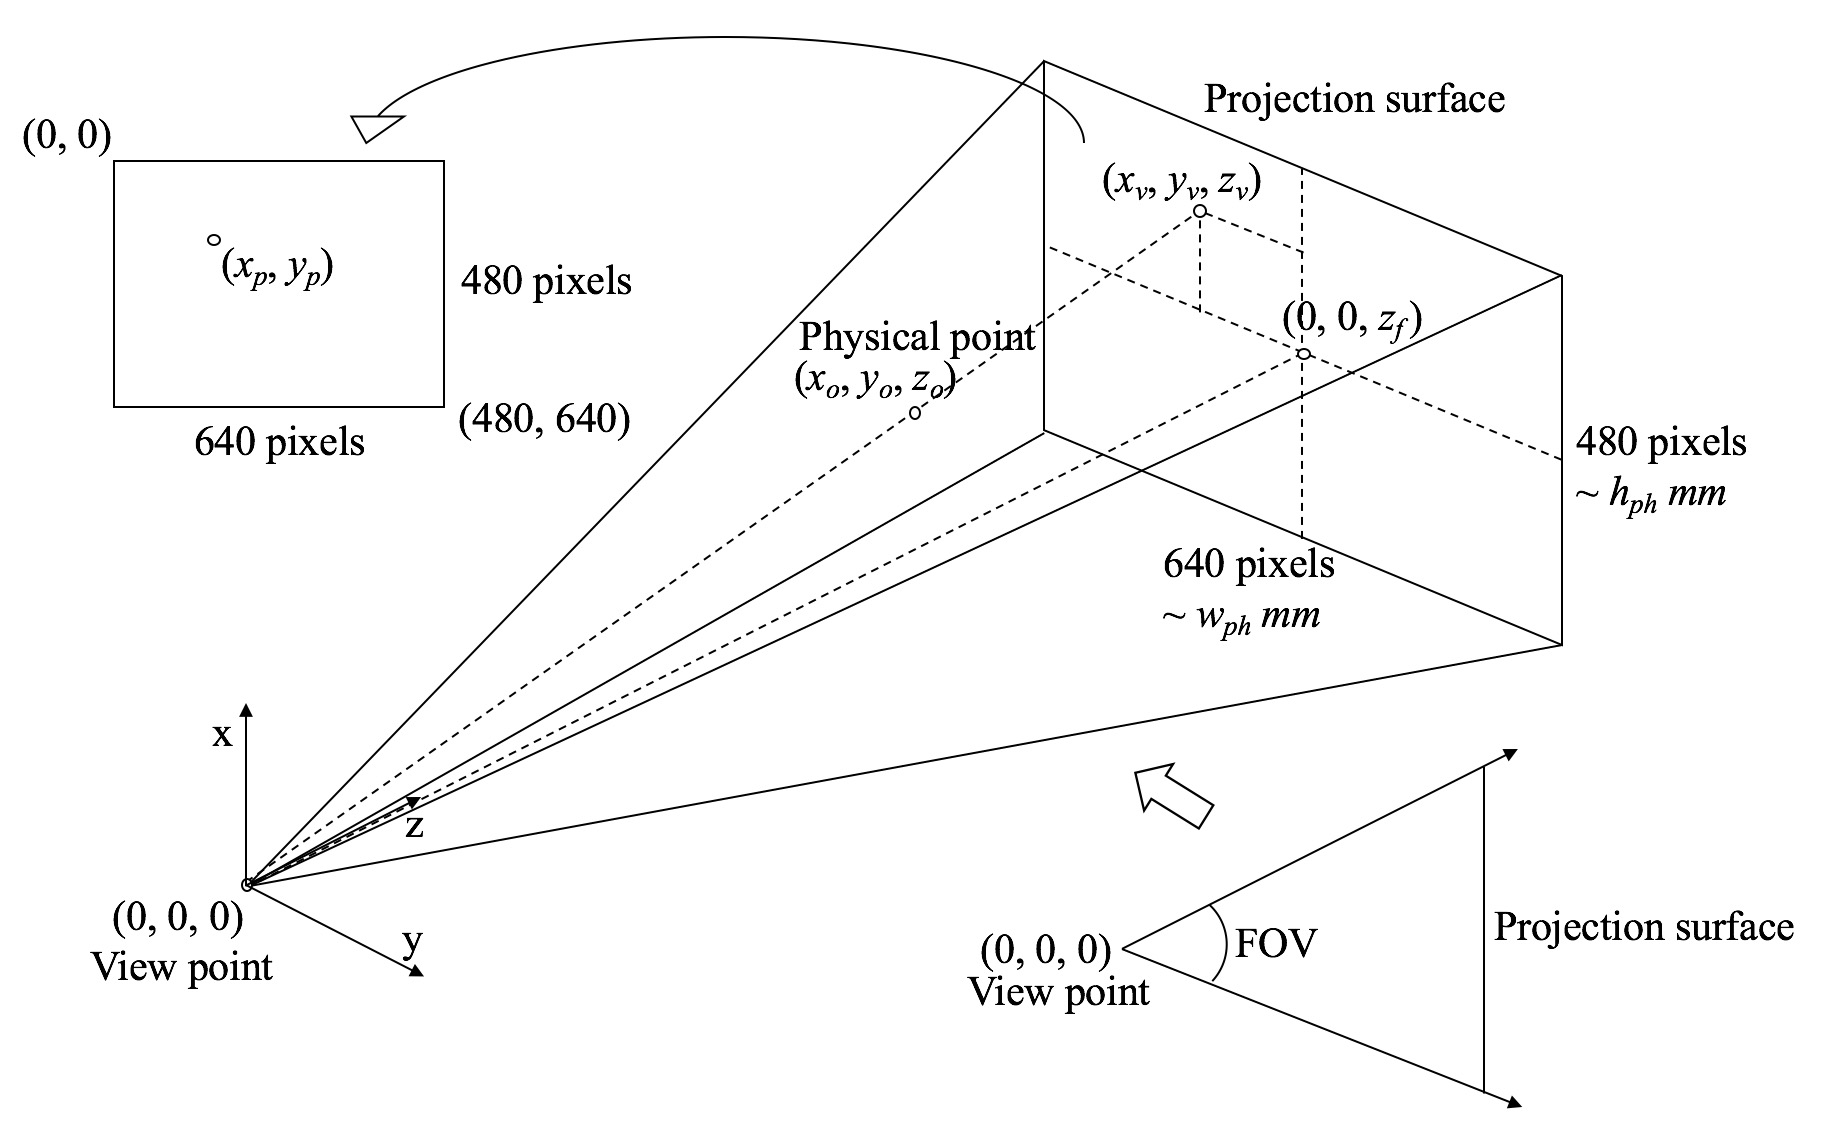
\includegraphics[width=\textwidth]{./mypic/projection.jpg} 
% 	\caption{} 
% \end{figure}
% \subsection{OpenGL原理} % stl文件、深度检测等等



\section{仿真环境搭建}
在有了上述投影变换的基本数学模型后,本节将继续阐述如何搭建一个实际的物理仿真平台。
\subsection{仿真流程及细节} % 
物体的3D模型文件是仿真环境中最重要的一个元素。3D文件可以有很多格式,例如3MF、STL、OBJ以及PLY等等文件格式,每种格式的文件都有其自身的特点,其中STL文件格式是一种非常通用简介的3D文件格式,并且与OpenGL平台相容性较好,因此本文就以STL文件为例进行阐述。

STL文件是由若干个三角形的相互连接定义组成,每个三角形平面的定义包括三角形各个顶点的三维坐标以及三角形平面的法向量,也就是这个三角形平面的朝向。其中这些顶点的三维坐标以及向量表达都是以该物体本身坐标系作为基准进行描述的,因此当我们需要仿真一个在空间中任意位置任意方向的物体的时候,需要将该物体的所有三角形坐标以及法向量进行变换。也就是存在一个物体坐标系到世界坐标系的变换:
\begin{equation}
	Cord_{obj}\to Cord_{world}
\end{equation}
描述这样一个变换通畅可以用六个维度进行定量衡量:X、Y、Z三个方向上的平移以及遵循一定顺序的X、Y、Z三方向的欧拉角旋转量。需要注意的是,仅仅给定了这六个变换参数也还是不能完全定义一个变换,还需要指定这些变换参数是在哪个参考系下进行的。本实验中采用的变换规则为:
\begin{enumerate}
\item 物体先以世界坐标系为基准进行X、Y、Z三个方向上的平移$\to State_1$
\item 物体以自身坐标系为基准,绕Z轴方向进行旋转$\to State_2$
\item 物体以自身坐标系为基准,绕X轴方向进行旋转$\to State_3$
\item 物体以自身坐标系为基准,绕Y轴方向进行旋转$\to State_4$
\end{enumerate}
例如给定了这六个参数分别为${d_x,d_y,d_z,a_x,a_y,a_z}$,并且初始情况下物体自身坐标系和世界坐标系重合,则物体坐标系下的一个点$P:{x,y,z}$经过变换后得到的世界坐标系下坐标可以有如下计算过程的到:

首先须要以自身坐标系为基准进行旋转,根据ZXY的顺序可以有旋转矩阵:
\begin{equation}
	R_{ZXY}=
	\begin{bmatrix} 
	cy\cdot cz-sy\cdot sx\cdot sz & cy\cdot sz+sy\cdot sx\cdot cz & -sy\cdot cx \\
	-sz\cdot cx & cz\cdot cx & sx \\
	sy\cdot cz+cy\cdot sx\cdot sz & sy\cdot sz-cy\cdot sx\cdot cz & cy\cdot cx 
	\end{bmatrix} 
\end{equation}
其中,$sx,cx,sy,cy,sz,cz$分别表示$sin(a_x),cos(a_x),sin(a_y),cos(a_y),sin(a_z),cos(a_z)$,旋转之后再进行平移便可得到最后世界坐标系下物体变换后的新坐标:
\begin{equation}
	P':\left[\begin{aligned}x' \\y' \\ z'\end{aligned}\right]=
	R_{ZXY}\cdot \left[\begin{aligned}x \\y \\ z\end{aligned}\right]+
	\left[\begin{aligned}dx \\dy \\ dz\end{aligned}\right]
\end{equation}
不同的变换顺序以及不同的基准坐标系都可以实现不同的变换,但在经过大量的实验测试之后可以发现,上述变换方式以及顺序与OpenGL默认环境最相容,在仿真过程中具有较强的直观感受,同时在计算上也具有较为简洁的中间步骤。

得益于OpenGL的Zbuffer机制,在对一个物体进行上述旋转变换后便可以很容易得到对应物体位姿下的深度仿真图以及对应的物体位姿真值。由于在OpenGL环境中,所有的深度数据都是通过Zbuffer来进行存储的,而Zbuffer的存储值取值范围受限于计算机仿真空间大小而被限制为$[0,1]$,其中0对应仿真环境中所能接受的最近点距离$near_z$,1对应仿真环境中所能接受的最远点距离$far_z$。因此这里存在一个转换关系:
\begin{equation}
	z=\frac{far_z\cdot near_z}{far_z - (far_z-near_z)\cdot z'}
\end{equation}
其中$z'$表示Zbuffer值$\to [0,1]$,$z$为真实物理长度距离。经过上式转换,就可以利用OpenGL环境得到最后真正的仿真深度图像。

下面为利用OpenGL进行深度图像仿真的基本流程图:
\begin{figure}[htb]
	\centering 
	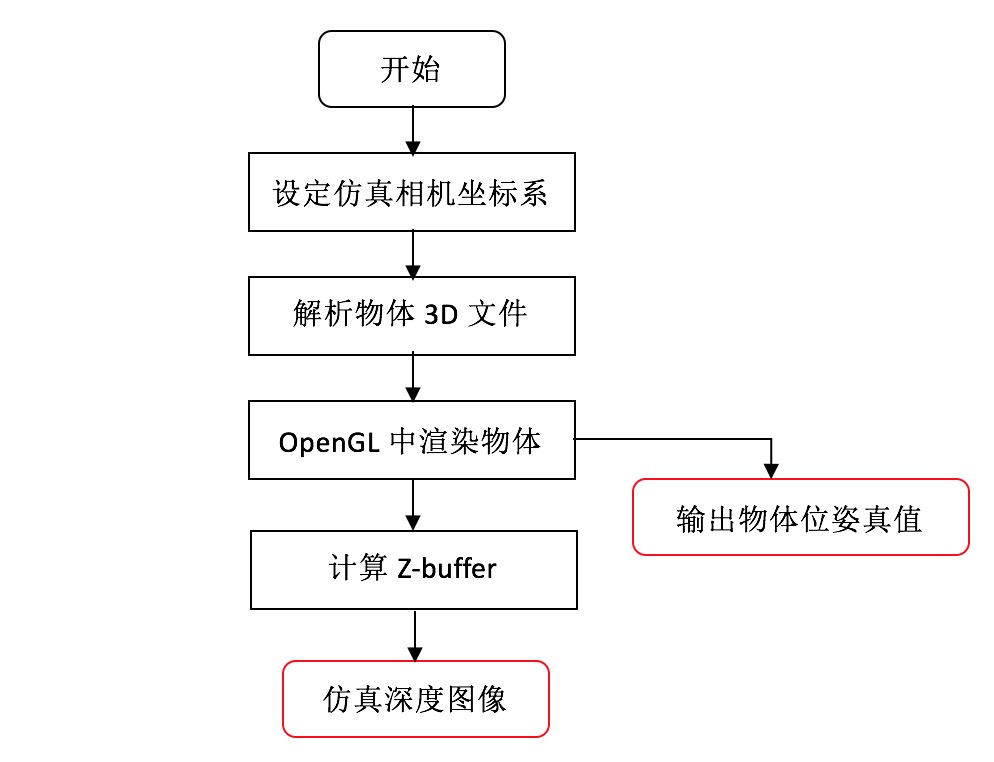
\includegraphics[width=0.7\textwidth]{./mypic/基于OpenGL深度图像仿真的基本流程示意图.jpg} 
	% 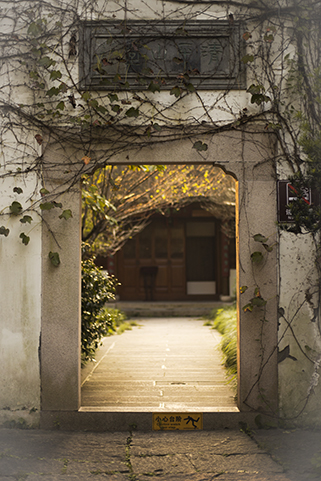
\includegraphics[scale=1.0]{./Pictures/test.jpg} 
	\caption{基于OpenGL深度图像仿真的基本流程示意图} 
\end{figure}





\subsection{模拟深度数据噪声} % 双高斯
可以发现,在上一小节中直接利用OpenGL可以得到非常完美的深度仿真图,该深度图像具有非常好的细节质量,没有任何噪声。但是对比下图可以发现,直接得到的深度图仿真图具有如下几个非常明显的缺点:

\begin{figure}[htb]
	\subfigure[原始仿真深度图像]{ 
		\begin{minipage}[b]{0.5\textwidth} 
		\centering
		% \label{fig:SubFigure1} %% label for second subfigure 
		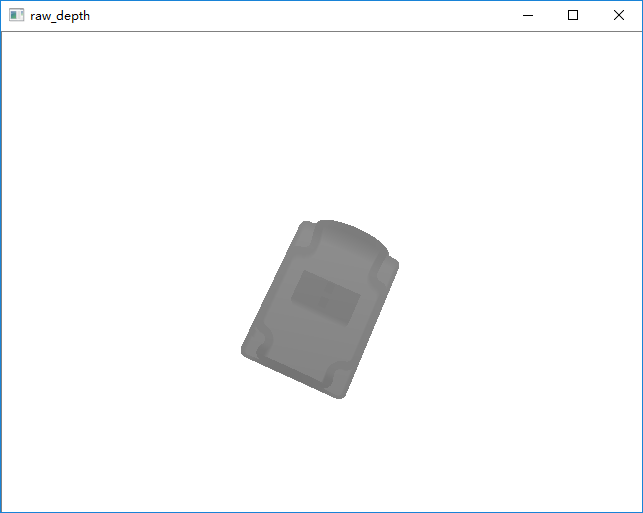
\includegraphics[scale=0.45]{./mypic/原始仿真深度图像.png} 
		\end{minipage}}
	\subfigure[深度相机下的真实深度图像]{ 
		\begin{minipage}[b]{0.5\textwidth} 
		\centering
		% \label{fig:SubFigure1} %% label for second subfigure 
		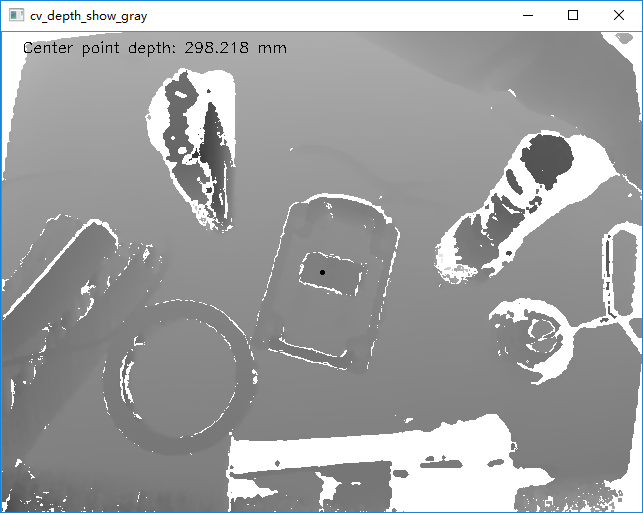
\includegraphics[scale=0.45]{./mypic/深度相机下的真实深度图像.png} 
		\end{minipage}}
	\caption{仿真深度图像与真实深度图像的对比}
\end{figure}

\begin{itemize}
\item 仿真深度图像非常光滑,没有任何噪声,但是真实深度图像有大量的噪声,即使是一个平面也会存在不平整的地方。
\item 仿真深度图像数据非常完备,所有像素点都存在数据,但是真实深度图像则有很多位置存在数据丢失,也就是真实深度图像存在数据空洞。
\item 仿真深度图像由于只仿真了物体本身的深度数据,除了物体本身的深度数据意外,其它位置的深度数据都是仿真环境的最远距离,没有实际意义。但是真实深度图像则有背景数据,甚至在一些情况下会有别的干扰物体对目标物体进行干扰或者遮挡。
\end{itemize}
上述问题的存在,使得仿真深度图由于太过完美而损失了大量真实性,对后续的仿真数据分析带来了极大的影响。因此本文针对这几点,提出了几个步骤对这些缺点进行修补,从而提高仿真图像的真实感,提升仿真真实性。

首先针对原始仿真图像没有任何噪声,极度光滑的问题,通畅可以采用模拟随机高斯噪声来解决。简单的高斯噪声可以通过对每一个像素点具有的深度值$d$附加一个均值为$0$,方差为$\sigma ^2$的高斯噪声得到。考虑到目前绝大多数的深度相机在测量上都存在一个和实际深度成正比的误差曲线,也就是随着被测物体的深度值越大,深度相机测量得到的深度信息携带的距离误差也会越大,因此此处$\sigma$应为一个与被测物体深度$\bar{d}$相关的函数,在本实验中采用下式表达形式:
\begin{equation}
	\sigma = \sqrt{\lambda \cdot \bar{d}}
\end{equation}
于是有:
\begin{equation}
	d'=d+N(0, \lambda \cdot \bar{d})
\end{equation}
但是,经过实验发现,仅仅采用简单的高斯噪声进行模拟得到的结果非常不理想。这样得到的仿真数据有非常明显的毛刺,在本该是平面的地方变得非常不光滑,或者说表面的法向量将存在非常严重的不连续性跳变。而实际深度图像中虽然存在噪声起伏,但是总体上还是平滑的,或者说表面法向量是基本不存在较大跳变的,如下图所示:

\begin{figure}[htb]
	\centering 
	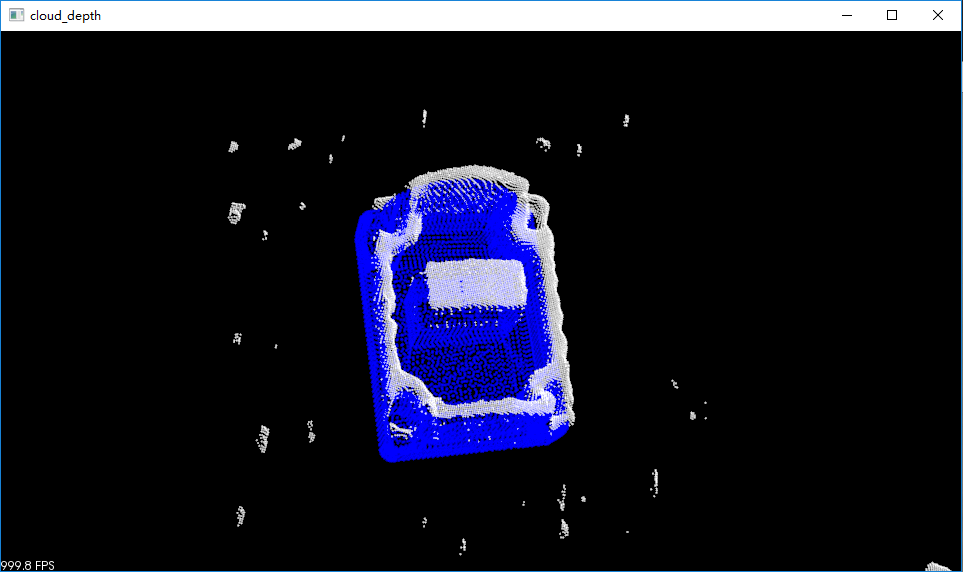
\includegraphics[width=\textwidth]{./mypic/实际深度相机下噪声的表现示意图.png} 
	% 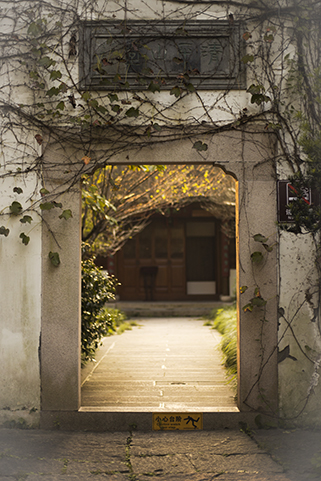
\includegraphics[scale=1.0]{./Pictures/test.jpg} 
	\caption{实际深度相机下噪声的表现示意图,为了方便展示,图中已经将深度图像转换为点云数据} 
\end{figure}

经过实验,本文最后采取适当调高$\lambda$的值,并在高斯噪声基础上套一层高斯平滑滤波。高斯平滑滤波可以采用一个比较大的高斯核进行操作,这样得到的混合高斯噪声就能有一个非常好的表现,既能够起到添加噪声的作用,同时也可以保证噪声的增加不会导致一些几何表面的眼中变形。最后可以用如下式子表示添加到原始仿真深度数据上的噪声:
\begin{equation}
	d'=d+Gaussian_{\Delta}(N(0, \lambda \cdot \bar{d}))
\end{equation}
其中$Gaussian_{\Delta}(\cdot)$表示对某一个$\Delta$区域上的高斯滤波操作。

针对第二点仿真深度图像没有空洞,但是实际深度图像存在较多空洞的问题。本文没有用直接的方法来生成空洞进行模拟,原因在于实际深度图像中很多的空洞的产生原因非常复杂,有外界环境红外光的干扰,也有物体表面材质的原因导致,如果直接通过随机的方式给仿真图像增加空洞,不光空洞大小会显得很突兀,空洞的形状也非常不好选择。因此,为了解决这个问题,本文采用逆向思维,通过修补真实深度图像数据中的空洞来使得其和仿真深度数据更加接近。

在大量的观察和对比,可以发现实际深度图像中绝大多数的空洞应有的深度值其实是和其周围数据接近或者完全一致的。也就是说这些空洞往往出现在物体的边界或者物体与物体之间的连接处,因此可以通过一些基本的图形学操作达到修补空洞的目的。基本的图形学操作有腐蚀、膨胀、开闭运算等。下图3-8展示了一个具有空洞的图形经过简单的膨胀图像操作,将空洞填满,本文也利用这一特性采用该方法对真实图像的空洞进行修补。

\begin{figure}[htb]
	\subfigure[原始图像]{ 
		\begin{minipage}[b]{0.5\textwidth} 
		\centering
		% \label{fig:SubFigure1} %% label for second subfigure 
		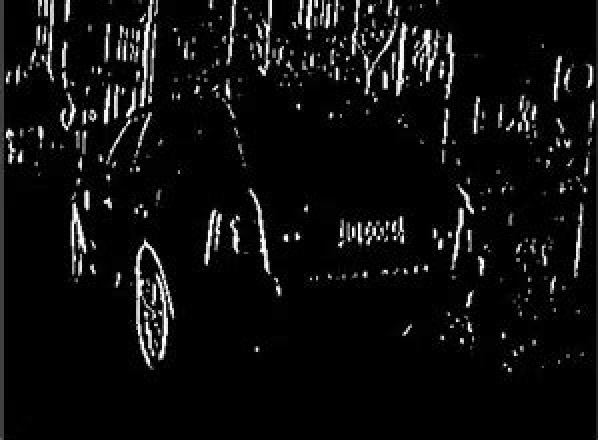
\includegraphics[scale=0.4]{./mypic/膨胀1.jpg} 
		\end{minipage}}
	\subfigure[经过膨胀操作后的图像]{ 
		\begin{minipage}[b]{0.5\textwidth} 
		\centering
		% \label{fig:SubFigure1} %% label for second subfigure 
		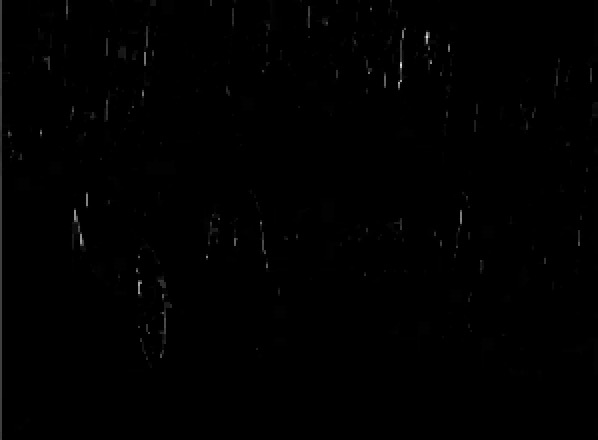
\includegraphics[scale=0.4]{./mypic/膨胀2.jpg} 
		\end{minipage}}
	\caption{图像的膨胀操作示意图}
\end{figure}

针对最后一点,实际深度图像具有背景以及前景遮挡等复杂环境而仿真环境得到的深度图像过于完美的情况。本文通过事先采集大量的背景深度数据(真实深度相机数据),随后将其叠加进原始仿真深度图像中去来解决复杂背景的模拟问题。用同样方法事先采集一些前景遮挡数据,并根据当前物体的仿真位置,将这些前景遮挡数据添加到其中进行模拟。其中,假设事先采集好的背景数据集合为$D_{bg}:\{d_{bg}^1,d_{bg}^2,...d_{bg}^n\}$,原始深度图像(经过噪声处理后的仿真深度图像)为$D_0$,则加入背景信息后的仿真深度图像可以表达为:
\begin{equation}
	D_1=union\{\ \max_{depth}\ (d_{bg}^i, D_0)\}
\end{equation}
进一步给定事先采集的前景数据集合为$D_{fg}:\{d_{fg}^1,d_{fg}^2,...d_{fg}^n\}$,物体在仿真环境中的位置为$P_{obj}$,则有加入前景遮挡信息后的仿真深度图像表示为:
\begin{equation}
\begin{aligned}
	\overline{d_{fg}^i} = F(P_{obj},d_{fg}^i)
	D_{final}=union\{\ \max_{depth}\ (\overline{d_{fg}^i}, D_1)\}
\end{aligned}
\end{equation}
其中$F(\cdot)$表示根据当前仿真物体的位姿调整前景物体信息到适当位置的变换函数,这个变换函数可以根据实际情况任意设置,因此不在此继续阐述。通过这种方式,在$F(\cdot)$尽量合理的情况下,就可以生成最后具有非常高仿真度的深度图像$D_{final}$。

图3-9整理为整个深度图像仿真流程概况图:

\begin{figure}[htb]
	\centering 
	\includegraphics[width=0.9\textwidth]{./mypic/基于OpenGL深度图像仿真的总流程示意图.jpg} 
	% \includegraphics[scale=1.0]{./Pictures/test.jpg} 
	\caption{基于OpenGL深度图像仿真的总流程示意图} 
\end{figure}




\newpage

\section{实验结果与分析}

按照上文所述的流程框架,本文在C++编程环境下完整搭建了该仿真深度相机平台,采用的物体3D模型文件格式为STL文件格式。通过解析STL文件中的三角面数据,添加入OpenGL环境中进行渲染,通过Z-buffer技术可以直接得到入图3-10所示的深度图像。
\begin{figure}[htb]
	\subfigure[]{ 
		\begin{minipage}[b]{0.5\textwidth} 
		\centering
		% \label{fig:SubFigure1} %% label for second subfigure 
		% \includegraphics[scale=0.4]{./mypic/膨胀1.jpg} 
		\includegraphics[scale=0.3]{./mypic/由物体的3D模型直接渲染得到的深度图像1.jpg} 
		\end{minipage}}
	\subfigure[]{ 
		\begin{minipage}[b]{0.5\textwidth} 
		\centering
		% \label{fig:SubFigure1} %% label for second subfigure 
		\includegraphics[scale=0.3]{./mypic/由物体的3D模型直接渲染得到的深度图像2.jpg} 
		\end{minipage}}
	% \caption{图像的膨胀操作示意图}
	% \includegraphics[scale=1.0]{./Pictures/test.jpg} 
	\caption{由物体的3D模型直接渲染得到的深度图像} 
\end{figure}

下一步,通过事先采集背景深度数据,利用通过公式3-17计算得到带有背景信息的仿真深度图像,如图3-11所示。以及利用公式3-18和事先采集的前景遮挡物信息,并为全图加入随机噪声后,可以得到入图3-12所示的最终仿真深度图像。

\begin{figure}[htb]
	\centering 
	\includegraphics[scale=0.22]{./mypic/加入背景深度信息之后的仿真深度图像.jpg} 
	% \includegraphics[scale=1.0]{./Pictures/test.jpg} 
	\caption{加入背景深度信息之后的仿真深度图像} 
\end{figure}

\begin{figure}[htb]
\centering 
\subfigure[]{\label{fig:subfig:a}
		\includegraphics[scale=0.11]{./mypic/最终仿真深度图像1.jpg} 
% \includegraphics[width=0.45\linewidth]{losebg_small}
}
\hspace{0.01\linewidth}
\subfigure[]{\label{fig:subfig:b}
		\includegraphics[scale=0.11]{./mypic/最终仿真深度图像2.jpg} 
% \includegraphics[width=0.45\linewidth]{losebg_small}
}
\vfill
\subfigure[]{\label{fig:subfig:a}
		\includegraphics[scale=0.11]{./mypic/最终仿真深度图像3.jpg} 
% \includegraphics[width=0.45\linewidth]{losebg_small}
}
\hspace{0.01\linewidth}
\subfigure[]{\label{fig:subfig:b}
		\includegraphics[scale=0.11]{./mypic/最终仿真深度图像4.jpg} 
% \includegraphics[width=0.45\linewidth]{losebg_small}
}
\caption{最终仿真深度图像示例}
% \label{fig:subfig}
\end{figure}

最后为了使仿真深度图像和真实的深度图像之间的差距更小,需要对真实图像中的深度缺失空洞进行填补。在本实验中,对两种方法进行了测试,一种为利用图形学方法对由空洞的深度图像进行膨胀处理,另一种为利用中值滤波的方式对空洞进行修补。从图3-13中可以看出,利用膨胀算法处理后的深度图像上空洞大大减少,并且仍旧能够保持物体本身原有的形状。但利用中值滤波的方式得到的深度图像依然存在较多的空洞。

因此本文在后续实验中采用的空洞修补方式均为图形学膨胀操作。

\begin{figure}[htb]
\centering 
\subfigure[原始真实深度图像]{\label{fig:subfig:a}
		\includegraphics[scale=0.7]{./mypic/空洞修补0.png} 
% \includegraphics[width=0.45\linewidth]{losebg_small}
}
% \hspace{0.01\linewidth}
% \subfigure[]{\label{fig:subfig:b}
% 		\includegraphics[scale=0.15]{./mypic/最终仿真深度图像2.jpg} 
% % \includegraphics[width=0.45\linewidth]{losebg_small}
% }
\vfill
\subfigure[膨胀处理下的深度图像]{\label{fig:subfig:a}
		\includegraphics[scale=0.7]{./mypic/空洞修补1.png} 
% \includegraphics[width=0.45\linewidth]{losebg_small}
}
\hspace{0.01\linewidth}
\subfigure[中值滤波下的深度图像]{\label{fig:subfig:b}
		\includegraphics[scale=0.7]{./mypic/空洞修补2.png} 
% \includegraphics[width=0.45\linewidth]{losebg_small}
}
\caption{对真实深度图像的空洞修补处理}
% \label{fig:subfig}
\end{figure}











\chapter{级联随机蕨回归框架下的物体六维位姿估计}

\section{概述}

在工业装配现场,为了实现生产过程的高效自动化,很多场合需要对工业零件或是一般物体进行自动化抓取或者放置。目前大多数场合下实现物体的自动化抓取以及放置采取的措施都是通过将被抓去或者放置的物体固定在一些具有非常高精度的位置上,并事先调试好硬代码来控制机械臂等执行机械进行操作。但这个方法需要大量的人力资源对工业现场进行部署,同时物体的位姿估计算法也须要针对每一个零件进行特殊的设计,大大降低了工业生产效率。因此下文将通过讨论一个新颖的物体位姿估计算法,来克服上述几个工业现场存在的问题。

本章的主旨是借鉴人脸特征点定位这个研究领域取得的杰出成果,提出一个更加通用高效的物体六维位姿估计算法框架。通过重新设计全新特征描述,使算法在深度图像上具有较高的信噪比,同时具备一定的尺度不变性。在第二章中已经给出了随机蕨算法的核心功能,本文将借助随机蕨回归算法,将其用于物体的六维位姿估计。其中,提出的新物体位姿估计算法框架需要大量的标记数据进行回归模型的训练,而第三章内容通过仿真深度相机可以在短时间内提供大量的此类数据,为该算法的研究提供了重要支撑。最后本文将进一步探讨遮挡情况下,利用大噪声干扰下的随机蕨回归算法进行异步位姿回归,从而克服遮挡情况对物体位姿回归的影响。

本章结构安排如下:4.2节内容主要讨论深度图像上的新特征设计,以及新特征的哈希处理。4.3节给出了物体位姿估计的主要流程框架以及框架中一些重要的实现细节。4.4节则进一步给出了如何将随机蕨算法改造后应用于遮挡情况下的物体位姿估计。最后通过实验逐一验证上述算法的可行性以及高效性。

\section{深度图像上的特征设计}

类似于SIFT、SURF、FAST等经典的特征描述一般都是针对RGB图像或者灰度图像进行设计的,这些特征描述能够反映出图像特征点周围的色彩或者纹理信息。这些特征点描述一般而言具有相对较高的计算复杂度,从而能够携带非常丰富的信息,因此具有非常好的稳定性。但在物体的位姿估计应用中这些特征描述就相对显得比较乏力,首先这些特征描述无法携带物体的深度信息,在描述深度图像中的特征点的时候不能够具有尺度不变性。也就是说对于物体的同一个特征点,不同的距离下,这些特征描述方法得到的结果都是不一样的。而我们通常希望在描述一个物体的同一个特征点的时候,不管该特征点距离深度相机的远近,都应该具有相同的特征描述。本文将主要针对这个问题介绍一种具有尺度不变性的全新特征描述。

\subsection{深度图像块的特征描述} % 

深度图像和传统RGB图像最本质的区别在于深度图像中每一个像素值反应的是这个位置的物体距离深度相机的距离,而不是这个物体的纹理信息。因此在对深度图像中的某一个位置进行特征描述的时候,应该充分考虑到这个位置本身的深度值,或者说在该处进行特征描述的过程应该是和该位置的深度值成一定函数关系的,如下式所示:
\begin{equation}
	F=D(I(x,y))
\end{equation}
其中$F$表示特征描述,$I$表示深度图像,$I(x,y)$表示在深度图像坐标$(x,y)$处对应点的深度值,$D(\cdot)$特征描述的具体表达形式。

另一方面,考虑到在物体位姿估计过程中,特别是针对工业现场下的物体位姿估计,物体都是具有相对稳定的结构,因此在进行一个物体的位姿描述的时候,不应该只局限于描述物体上某一个点周围的纹理信息,而应该考虑到将整个物体的概况整体描述进特征里。也就是说,在深度图像上进行特征描述的过程,应该是针对一个局部深度图像块的,这个深度图像块的大小根据透视变换的几何性质应该正比于该位置的深度值平方:
\begin{equation}
\begin{aligned}
	& D(I(x,y))\equiv{D_\Delta}(I(x,y)) \\
	& \Delta\propto{I^2(x,y)}
\end{aligned}
\end{equation}

这一点应该类似于目前较为成熟的人脸特征点定位中的特征描述。在对人脸特征点进行定位过程中,由于人脸具有非常强的对称性,脸部很多地方存在局部相似,如果不考虑整个人脸的整体信息进行直接定位回归的话会导致算法极易陷入局部极小值而失败。目前人脸特征点定位领域中表现最好的算法采用的特征描述称为差值形状索引特征(Interpolated shape-indexed features)\cite{burgos2013robust}。如下图所示:
\begin{figure}[htb]
	\centering 
	% \includegraphics[width=\textwidth]{./Pictures/test.jpg} 
	\includegraphics[width=0.8\textwidth]{./mypic/人脸特征描述方法.jpg} 
	\caption{人脸特征描述方法中的差值形状索引特征} 
\end{figure}
图中人脸形状由人脸特征点列构成(图中十字点,为了方便阐述仅画出两个),任意取特征点列中的两个点作为基础点,给一个随机比例差值可以得到一个新的点。所有这些通过差值得到的点像素构成一个集合,两两像素值做差便得到了基础特征描述库。可以看出,在人脸特征点定位中用到的特征描述具有非常简洁的形式:
\begin{equation}
	f_{p_1,p_2}(I)=I(p_1)-I(p_2)
\end{equation}
但事实证明,这样简洁的特征描述确实能够很好地表达出人脸面部特征,并能以此回归出非常精准的特征点定位结果。本文认为这样的特征描述之所以能有非常好的表达能力,关键在于基础特征库的生成是通过整体特征点差值得到的。这一步骤不仅仅能将人脸整体的概况信息包含进去,同时也能够通过差值的方式反映出人脸局部的一些结构信息,实现了从概况到细节的所有信息的融合。因此,本文受该特征描述的启发,结合深度图像本身的特点提出一种全新的特征描述方式。
\begin{figure}[htb]
	\centering 
	% \includegraphics[width=\textwidth]{./Pictures/test.jpg} 
	\includegraphics[width=\textwidth]{./mypic/物体位姿估计特征描述方法.jpg} 
	\caption{物体位姿估计特征描述方法} 
\end{figure}

在给定物体的大致位置后(深度图像中该物体的中心点像素坐标),首先由公式(4-2)给出的关系确定特征描述块的大小,使得特征描述框能够覆盖整个物体。实际算法部署过程中,会事先人为标注一个标准距离$d_0$下特征描述框的大小$S_0$,当遇到新场景下实际物体距离为$d'$时,可以直接计算出新的特征描述框大小:
\begin{equation}
	S'=\left(\frac{d'}{d_0}\right)^2\cdot S_0
\end{equation}

下一步须要将得到的特征描述框进行划分。首先将其均分成5*5个子方块,每个子方块相互紧挨覆盖整个特征描述框,如图4-2中间黑线划分方式。然后再在原始特征描述框的中部取4*4个子方块,每个子方块的大小与先前黑线划分得到的子方块大小相同,并且这16个子方块中的每一个方块都位于黑线划分得到的其中4个方块的交界处。这样总共可以得到41个特征描述框子区域。

得到上述这41个子区域之后,将这41个子区域进行平均采样25个像素点(如图4-2最右侧所示),第$A_k$个子区域上的点记为$\{d_{k_1},d_{k_2},...,d_{k_n}\}$,总共可以得到1025个特征样本点。但这些像素点的深度值信息过于简单,不能直作为特征,需要进一步处理。对于每一个子区域上的25个像素点,我们计算其深度均值$\bar{d}_k$,并将这25个像素点的深度值减去$\bar{d}_k$。这样在每一个子区域中,串联所有的深度值之差以及该深度均值可以得到一个26纬度的子特征,总共可以得到1066维度的特征。然后继续计算上述所有子区域中采样得到的深度均值的均值:
\begin{equation}
	\bar{d}_{all}=\frac{1}{41}\sum_{k=1}^{41} \bar{d}_k
\end{equation}
再将这41个子区域的均值减去$\bar{d}_{all}$得到另外25维度特征,最后加上$\bar{d}_{all}$本身,一共可以得到1092维度的特征描述。

通过这样将整个特征描述区域进行拆分采样,最后通过相互取均值做差的方式进行特征整合描述,可以充分描述出整个区域上的深度分布情况,同时也将局部特征信息包含进特征描述中形成一个具有非常完备的特征描述形式。并且由于特征描述区域大小是通过实际的深度值计算得到的,因此这种特征描述方式具有很好的尺度不变特性。

\subsection{特征哈希处理} % 

为了使特征描述有更高的信噪比,需要对特征进行降维或者哈希化处理。本文借鉴了F. Shen等人在2015年CVPR中提出的监督学习下的哈希算法\cite{shen2015supervised},通过适当简化其算法过程,提高其算法效率的同时保持其哈希处理的高信噪比优势。

假设存在$n$个特征样本$X=\{x_i\}^{n}_{i=1}$,并且期望将其在监督学习下降维得到长度为$L$的二进制编码$B=\{b_i\}^{n}_{i=1}\in\{-1,1\}^{L\times n}$来代替它,其中$b_i$表示$x_i$的第$i$列二进制码。同时假设在线性分类情况下,有如下式所示的多分类问题:
\begin{equation}
	y=G(b)=W^{\top}b=\left[w_1^\top,...,w_c^\top\right]^\top
\end{equation}

其中$w_k\in \Re^{L\times 1},k=1,...,C$为第$k$类分类向量,$y\in \Re^{C\times 1}$为类别标签向量。显然,上述问题可以等价于求解下式所示的优化问题:
\begin{equation}
\begin{aligned}
	& \min_{B,W,F} \sum_{i=1}^n L\left(y_i,W^\top b_i\right)+\lambda \|W\|^2 \\
	& \ s.t. \  b_i=sgn\left(F(x_i)\right),i=1,...,n.
\end{aligned}
\end{equation}

这里$L(\cdot)$为损失函数,$\lambda$为正则参数,$Y=\{y_i\}_{i=1}^n\in\Re ^{C\times n}$为真值矩阵。这里将二进制限制放宽为连续函数$F(x)$,同时引入二进制损失项可以得到最后的优化问题如下:
\begin{equation}
\begin{aligned}
	& \min_{B,W,F} \sum_{i=1}^n L\left(y_i,W^\top b_i\right)+\lambda \|W\|^2 + \nu\sum_{i=1}^n \|b_i-F(x_i)\|^2     \\
	& \quad\quad\quad\quad\quad\quad\quad s.t. \  b_i\in\{-1,1\}^L.
\end{aligned}
\end{equation}

此处本文考虑到计算效率,采用线性学习算法来直接构建$F(x)$:
\begin{equation}
\begin{aligned}
	& \quad\quad\quad\quad\quad\quad F(x)=P^\top\phi(x) \\
	& \phi(x)=\left[\exp(\frac{\|x-a_1\|^2}{\sigma}),...,\exp(\frac{\|x-a_m\|^2}{\sigma})\right]
\end{aligned}
\end{equation}
这里$\{a_j\}_{j=1}^m$是从训练样本里随机选择的$m$个锚点。接下来将取$L_2$作为损失函数,分为3步对该问题进行求解:G-Step,F-Step,B-Step:
\begin{itemize}
\item G-Step: 固定$B$,可以以最小二乘形式得到$W$:
\begin{equation}
	W=(BB^\top+\lambda I)^{-1}BY^\top
\end{equation}
\item F-Step: 固定$B$,可以得到$P$:
\begin{equation}
	P=\left(\phi(X)\phi^\top(X)\right)^{-1}\phi(X)B^\top
\end{equation}
\item B-Step: 固定除$B$之外的所有变量,采用DCC算法(discrete cyclic coordinate descent method),可以对$B$进行逐位求解:
\begin{equation}
	B: z=sgn(q-B'^\top W'\nu)
\end{equation}
\end{itemize}
其中$z^\top$表示$B$的第$l$行,$B'$表示矩阵$B$除开$z$后的子矩阵,$q^\top$表示$Q=WY+\nu F(X)$的第$l$行,$Q'$表示矩阵除开$q$后的子矩阵,$\nu^\top$表示$W$矩阵的第$l$行,$W'$表示$W$矩阵除开$\nu$后的子矩阵。

在实际应用过程中,通过不断迭代循环上述三个步骤,代入计算$W$,$P$以及$z$,便可逐步收敛,得到最后的哈希码$B$。

但由于在这个算法中锚点的计算会消耗大量的计算资源,为了提高回归算法的效率,本文舍弃锚点的选取,直接采用原始特征信息作为训练的数据,并同时采用回归目标值作为学习目标直接带入算法,不再将回归目标值映射到分类问题上进行处理。通过上述步骤就可以得到下文所需要用到的用于位姿回归拟合的最终哈希特征。

\section{针对位姿估计的级联回归框架设计}

在传统级联回归框架中,所有级联层之间的功能都是一样的,包括具有完全相同的回归拟合器,也包括完全相同的回归目标。例如,在目前表现最优秀的人脸特征点定位算法中\cite{chen2014joint},采用改进的随机森林作为回归器,回归目标为每一级回归器当前的特征点坐标与真值之间的偏差。并且,在训练每一级回归器的时候用到的回归器训练参数也都是完全一致的。这样的级联回归框架有如图4-3所示的大致结构。

\begin{figure}[htb]
	\centering 
	\includegraphics[width=0.6\textwidth]{./mypic/经典级联回归算法流程图.jpg} 
	% \includegraphics[scale=1.0]{./Pictures/test.jpg} 
	\caption{经典级联回归算法流程图} 
\end{figure}

但是在物体的位姿估计问题下,需要回归的目标并不是单纯的某些像素值在图像上的坐标,而是比较抽象的物体的六维空间朝向以及空间坐标。这些抽象的回归目标不能在图像上得到直接的反馈,这就会导致下面这样一个问题:
\begin{itemize}
\item 如果采用各级回归模型都完全一致的级联回归框架,并且每一级的回归器训练目标都直接为物体的当前六维位姿。那么将有如下回归优化目标:
\begin{equation}
\begin{aligned}
	& R^t=\arg \min_R \sum_i \|\hat{S}_i-(S_i^{t-1}+R(x_i,S_i^{t-1}))\|^2. \\
	& S:\{dx,dy,dz,d\theta_x,d\theta_y,d\theta_z\}
\end{aligned}
\end{equation}
其中$R$表示各级的回归拟合器,$S_i$表示当前第$i$级物体的六维位姿,$\hat{S}_i$表示位姿的真值,$x_i$表示当前特征描述框。

结合上一节所述,可以很明显看出,在每一级的位姿估计结果$S_i$更新迭代过程中,至少有这三个维度的更新迭代是没有意义的:$\{d\theta_x,d\theta_y,d\theta_z\}$。也就是说,每当一级回归器得到了回归结果之后,虽然可以更新目标物体的当前位姿,但是目标物体当前的位姿对下一级的回归所需要的特征描述所需要的前提是过饱和的。因为按照上节所述的特征描述方法,仅仅需要得知当前物体在深度图像中的质心像素位置即可,也就是仅仅需要$S$中的前三个空间坐标$\{dx,dy,dz\}$。这样一来,如果级联回归框架中每一级都采用完全相同的回归目标的话,就会产生极大的计算资源浪费,大大降低算法的效率,同时回归目标维度的增加也会大大提高回归器训练所需要的时间,甚至可能导致回归器无法得到可靠的回归结果。
\end{itemize}

为了解决上述问题,本文考虑将原始的级联回归框架拆分成两部分,第一部分用于回归物体的质心空间坐标,第二部分用于回归物体的欧拉角位姿。其中第一部分中,由于物体质心空间坐标可以由第三章中的投影关系给出其与深度图像中像素位置的对应关系,这一部分的回归问题可以转化为标准级联回归问题。而第二部分的回归问题较为复杂,是无法转化为级联回归问题的。但得益于第一部分与第二部分的耦合,如果在第一部分问题得到较好的解决情况下,也就是一旦物体的质心空间位置已经得到了较好的估计,在此基础上再进行物体的空间姿态估计将变为地较为容易,回归目标的复杂度也大大降低。因此,可以考虑使用一个相比质心空间坐标回归器稍微强一点的回归拟合器对物体的欧拉角位姿进行直接拟合。

最后将第一部分的基础级联回归器与第二部分的强回归拟合器按先后顺序再次级联,便可以得到物体位姿估计问题下的最终级联回归算法框架。下图为该复合式级联回归框架的流程图:

\begin{figure}[htb]
	\centering 
	\includegraphics[width=0.6\textwidth]{./mypic/复合式级联回归框架的流程图.jpg} 
	% \includegraphics[scale=1.0]{./Pictures/test.jpg} 
	\caption{复合式级联回归框架的流程图} 
\end{figure}


\section{遮挡情况下的物体位姿估计} % 如何估计物体的被遮挡情况

复杂环境下的物体位姿估计一直以来都是物体位姿估计领域一个重要的难点。当物体在杂乱的环境中,或者工业现场一些零件的堆放过于散乱,会出现物体或者零件被遮挡的情况。结合上文中的特征描述方法,不难得到,一旦物体被局部遮挡,特征描述就会受到极大的干扰。

\begin{figure}[htb]
	\centering 
	\includegraphics[width=0.5\textwidth]{./mypic/物体存在被遮挡的情况.png} 
	% \includegraphics[scale=1.0]{./Pictures/test.jpg} 
	\caption{物体(红色点区域)被遮挡的情况示意图} 
\end{figure}

如上图所示,物体被遮挡将直接导致特征基础库中的像素值完全失去可信度,并且当这些被污染的特征传入后续的随机蕨算法中时,会大大干扰随机蕨算法的最后结果,导致最后物体位姿估计结果发生较大的偏差。因此,本文考虑引入第二章内容所讲的大噪声干扰下的随机蕨算法,利用其掩码的性质来克服物体被遮挡后的位姿回归问题。

由于掩码机制的存在,特征降维操作将不再适用此处,因为如果采用4.2.2节中所用的特征降维方法,经过中间的迭代步骤,会导致最后的哈希特征所有维度都会被污染。而经过实验验证,如果采用未降维的特征作为最后位姿估计的特征,其对应的特征掩码是可以被估计出来的。

在位姿估计这个问题下,要对特征掩码进行预测首先要先对物体的被遮挡情况进行估计。选取经典的随机蕨分类器,以4.2.1中所述的特征描述作为该分类器的输入,以特征描述区域上的1025个采样点被遮挡情况作为输出,并利用第三章中提到的仿真环境给出的大量有真值标注的数据进行分类器训练,就可以得到我们所需要的掩码估计初步结果。如下式所示:
\begin{equation}
\begin{aligned}
	& M: \left[m_1,m_2,...,m_1025\right]^\top
	& M_i=Classifier_i(F)\in[0,1]
\end{aligned}
\end{equation}

上式中得到的$M_i$在实际计算过程中不能完全取值到严格的0(意味该采样点被遮挡)或者1(意味该采样点为被遮挡),最后的结果是概率化的表达。之后,由于最终的1092维特征所有的维度都是通过这些采样点相互计算得到,因此这1092维特征可以用如下公式来计算其相应的置信度掩码:
\begin{equation}
	W=weight(M)=\frac{\sum M_i\cdot relevant(i)}{S}
\end{equation}
其中,$W$为最后的特征置信度掩码$relevant(\cdot)$函数用来表示该采样点与当前特征维度的相关度,$S$表示当前采样点用到的计算数,例如当前特征维度需要由$k$个基础采样点计算得到,则此处$S$取值就为$k$。当然,由于在本文中的特征描述具有固定的特性,此处$relevant(\cdot)$函数的计算其实可以通过预先计算得到,通过查表的方式得到,从而可以提高算法的效率。

注意上文得到的最后的特征置信度掩码最后的表现形式也是概率化的。有了特征描述以及其对应的特征置信度掩码后,就可以套用本文2.3节中阐述的改进后的随机蕨回归算法代替原先位姿估计框架中的基础随机蕨回归算法,得到可以应对遮挡情况下的物体位姿估计方法。其最后的流程图如下图所示:

\begin{figure}[htb]
	\centering 
	\includegraphics[width=0.75\textwidth]{./mypic/有遮挡情况下的物体位姿级联回归框架流程图.jpg} 
	% \includegraphics[scale=1.0]{./Pictures/test.jpg} 
	\caption{有遮挡情况下的物体位姿级联回归框架流程图} 
\end{figure}


\section{物体检测与物体位姿估计的结合}

前文所述的物体位姿估计算法框架的前提是需要被测物体具有一个较为理想的初始空间坐标。而通常情况下,这个初始空间坐标是不存在的,因此本文提出一种简洁的办法来解决这个问题。

物体的初始空间坐标映射到深度图像中为一个像素点位置,因此给出初始空间坐标本质上可以等价于深度图像上的物体检测问题。物体检测问题通常情况下不外乎物体的特征描述以及一个标准的分类问题。注意到本文在4.2节中提出的特征描述具有非常好的信息表达能力,同时随机蕨算法本身又是一个非常强大的分类器算法。因此可以直接利用本文提出的特征描述,附加一个简单的随机蕨分类器作为物体检测模块。

利用上述方法进行物体检测有一个很自然的特点,就是物体检测与位姿估计所用的特征描述完全一致。这也意味着当物体在深度图像中被检测到时,不需要再重新计算一边特征描述用于位姿估计,从而大大提高算法整体的效率。这个特性是传统方法所不具备的,传统方法往往将物体检测与物体位姿估计两者的特征描述分开设计,效率极低。

本文采用的物体检测采用最基本的滑动窗口方式进行,由于特征描述本身具有一定的描述范围,并且在一个深度情况下只可能存在一个被测物体,因此滑动窗口只需要设置一层,并且按照一定的间隔排布即可:

\begin{figure}[htb]
	\centering 
	\includegraphics[width=0.7\textwidth]{./mypic/滑动窗口示意图.jpg} 
	% \includegraphics[scale=1.0]{./cyk/test.jpg} 
	\caption{滑动窗口示意图} 
\end{figure}
通过该方法检测到物体的初始状态之后便可以直接作为物体位姿估计算法的初始条件进行后续位姿估计。

\section{实验结果与分析} % 物体检测放在这里讲

\subsection{利用物体位姿特征进行物体检测实验}

本文实验过程中采用的深度相机为Intel公司生产的RealSense SR300系列深度相机,其具备分辨率为640*480大小的红外深度传感器,通过USB接口可以方便获取其深度图像数据。通过人为随机移动该深度相机,使其围绕被检测物体,在此期间持续采集深度图像数据作为本实验的数据来源。此方法下,可以保证物体每一帧都存在于深度图像中,并且有位姿各异的情形。实验中,定义查准率 (precision) 作为评估物体检测能力的好坏。查准率$P$为物体检测器检测到目标人的帧数占所采集到的总帧数的百分比。

本文一共对4种物体进行了试验,每一种物体采集了约1500帧深度图像数据,采用经典随机蕨算法作为物体分类器,滑动窗口步长设为对应特征描述区域宽度的一半,得到具体结果如下表所示:

\begin{table}[htb]
	\zihao{5}
	\caption{利用物体位姿估计特征进行物体检测实验} 
	% \label{Tabkeyword}
	\centering 
	\begin{tabular}[t]{
		% |c|l|r|p{4cm}|} 
		ccccccc} 
		\toprule
		物体类别 & 成功检测帧数 & 总帧数 & 查准率\\ 
		\midrule
		开关零件盒底座 & 1502 & 1524 & 98.56\% \\
		羽毛球模型 & 1664 & 1681 & 98.99\% \\
		小黄鸭模型 & 1542 & 1556 & 99.10\% \\
		水壶模型 & 1583 & 1604 & 98.69\% \\
		\bottomrule
	\end{tabular}
\end{table}

从表4-1可以看出,利用物体位姿估计特征进行物体检测在实验中4个样本物体上都取得了高于98\%的查准率,可见该方法的合理性。并且,经过复查,几乎所有的漏检案例中,导致分类器漏检的原因都是由于被检测物体在特定的角度下表面材质反光,在深度图像上形成了巨大的空洞,从而使提取到的特征严重失真。

但另一方面,本实验也有一定的不足之处。由于实验场所有限,背景信息并不复杂,干扰物少,使得分类器在区分前景和背景的过程中几乎没有困难,从而导致物体的查准率能够如此之高。但对于工业场景而言,该方法有足够的能力完成物体检测任务,毕竟在工业场景中不会出现非常复杂的背景。

\subsection{无遮挡情况下的物体六维位姿估计实验}

本文采用4.3节所述的位姿估计算法框架,在C++编程环境下实现了该算法。并通过自己制作了一套数据集对该算法进行了评估。

数据集主要包含两个真实物体在深度相机下各个朝向的位姿,以及对应位姿下深度相机采集到的深度图像数据。不像仿真环境数据可以直接获取物体在空间中的位姿,为了得到真实数据集中各个物体的真实位姿,本文采用ARTag技术协助标注真实位姿。如图4-8所示,将物体固定在ARTag标定板的中间,通过RGB相机可以方便的计算出ARTag板相对于相机的空间位姿,进一步空间坐标换算可以粗略的得到物体相对于深度相机坐标系下的位姿。在有了粗略的相对位姿后,可以通过将物体的3D模型反投影到对应的深度图像中,以点云的方式对物体的位姿进行微调最后得到精准的数据集样本。
\begin{figure}[htb]
	\centering 
	\includegraphics[width=0.7\textwidth]{./mypic/数据集制作.png} 
	% \includegraphics[scale=1.0]{./cyk/test.jpg} 
	\caption{数据集制作示意图} 
\end{figure}

由于数据集制作需要的时间耗费巨大,截止本文撰写时仅仅完成了对一个物体的数据集制作,因此本文更多的实验数据来自于仿真环境给出的仿真数据。

在真实数据集上测试的效果如表4-2所示,其中数据集内含标注样本数量487个,着重与文章[\citenum{drost2010model}]中的方法进行了比较。在仿真数据集上进行测试的效果如表4-3所示,其中数据集包含7种物体,每种物体样本数量为500个。
\begin{table}[htb]
	\zihao{5}
	\caption{真实数据集上测试的位姿估计精度表现} 
	% \label{Tabkeyword}
	\centering 
	\begin{tabular}[t]{
		% |c|l|r|p{4cm}|} 
		ccc} 
		\toprule
		方法类别 & 本方法 & 文章[\citenum{drost2010model}]\\ 
		\midrule
		X方向平移误差(单位:mm) & 1.35 & 0.59\\
		Y方向平移误差(单位:mm) & 0.83 & 0.71\\
		Z方向平移误差(单位:mm) & 1.95 & 1.41\\
		X方向欧拉角误差(单位:度) & 2.30 & 1.85\\
		Y方向欧拉角误差(单位:度) & 1.31 & 2.25\\
		Z方向欧拉角误差(单位:度) & 1.13 & 3.36\\
		\midrule
		失败率 & 0\% & 67.4\% \\
		\midrule
		算法速度 & 30fps & 0.46fps \\
		\bottomrule
	\end{tabular}
\end{table}

\begin{table}[htb]
	\zihao{5}
	\caption{仿真数据集上测试的位姿估计精度表现} 
	% \label{Tabkeyword}
	\centering 
	\begin{tabular}[t]{
		% |c|l|r|p{4cm}|} 
		cccccccc} 
		\toprule
		物体类别 & 开关零件盒底座 & 开关零件头 & 羽毛球 & 小黄鸭 & 水壶 & 茶杯 & 相机\\ 
		\midrule
		X方向平移误差(单位:mm) & 1.13 & 0.97 & 0.99& 1.30& 1.16&1.22 &1.06 \\
		Y方向平移误差(单位:mm) & 0.78 & 0.81 & 1.16&1.05 &1.19 &1.02 &1.15 \\
		Z方向平移误差(单位:mm) & 0.95 & 1.02 & 1.08& 1.08& 0.97& 1.30&1.20 \\
		X方向欧拉角误差(单位:度) & 1.81 & 1.55 &1.30 &1.09 &1.98 &1.76 &1.15 \\
		Y方向欧拉角误差(单位:度) & 1.11 & 1.01 &1.40 &1.27 &1.50 &1.24 &1.82 \\
		Z方向欧拉角误差(单位:度) & 1.03 & 1.38 &1.16 &1.38 &1.13 &1.59 &1.60 \\
		\bottomrule
	\end{tabular}
\end{table}

从表4-2中可以看出,本文提出的方法在物体位姿估计的精度上相比文章[\citenum{drost2010model}]要稍显不足,主要表现在质心空间坐标的位姿估计精度不够以及X方向欧拉角误差较高。但相比于文章[\citenum{drost2010model}],本文提出的方法具有两个重大优势,第一点在于本文方法的失败率极低,能够应对绝大多数情况下的位姿估计问题,而文章[\citenum{drost2010model}]则由于算法上的缺陷,有67.4\%情况下无法得到物体的位姿结果。第二点在于算法的效率,本文方法借助高效的特征描述以及随机蕨级联回归框架能够达到每秒处理30帧数据的速度,做到实时物体位姿估计,这是文章[\citenum{drost2010model}]无法做到的。

对比表4-2与表4-3,可以发现在真实数据集上测试的效果与仿真数据集上测试的效果差别并不大,这一点表明了仿真环境得到的深度图像数据与真实环境中的差别已经很小了。同时,表4-3中7个物体的位姿估计精度差别也都保持着非常接近的数据,这表明了本文所提的这套级联位姿估计算法框架的合理性以及通用性。图4-9展示了一些真实数据集上的位姿估计可视化结果,其中绿色方框表示物体位姿的真值,红色方框表示物体的位姿估计结果。

\begin{figure}[htb]
\centering 
\subfigure[]{\label{fig:subfig:a}
		\includegraphics[width=0.4\linewidth]{./mypic/94.png} 
% \includegraphics[width=0.4\linewidth]{losebg_small}
}
\hspace{0.01\linewidth}
\subfigure[]{\label{fig:subfig:b}
		\includegraphics[width=0.4\linewidth]{./mypic/95.png} 
% \includegraphics[width=0.4\linewidth]{losebg_small}
}
\vfill
\subfigure[]{\label{fig:subfig:a}
		\includegraphics[width=0.4\linewidth]{./mypic/96.png} 
% \includegraphics[width=0.4\linewidth]{losebg_small}
}
\hspace{0.01\linewidth}
\subfigure[]{\label{fig:subfig:b}
		\includegraphics[width=0.4\linewidth]{./mypic/98.png} 
% \includegraphics[width=0.4\linewidth]{losebg_small}
}
\vfill
\subfigure[]{\label{fig:subfig:a}
		\includegraphics[width=0.4\linewidth]{./mypic/99.png} 
% \includegraphics[width=0.4\linewidth]{losebg_small}
}
\hspace{0.01\linewidth}
\subfigure[]{\label{fig:subfig:b}
		\includegraphics[width=0.4\linewidth]{./mypic/100.png} 
% \includegraphics[width=0.4\linewidth]{losebg_small}
}
\caption{一些真实数据集上的位姿估计可视化结果}
% \label{fig:subfig}
\end{figure}

\newpage

\subsection{有遮挡情况下的物体六维位姿估计实验}

本文根据4.4节内容所提方法进一步改进物体六维位姿估计算法,对物体被遮挡时的位姿估计进行了实验。首先验证了是否能够通过原始特征拿到物体当前状态下被遮挡的情况,本文采用经典随机蕨分类器作为基本工具,采用第三章所提的仿真数据训练了一个遮挡情况预测器。如图4-10所示,在零件周围随机撒点,预测器能够顺利预测出物体被遮挡的情况,在图中被遮挡的位置用绿色点标出。
\begin{figure}[htb]
	\centering 
	\includegraphics[width=0.7\textwidth]{./mypic/1.png} 
	% \includegraphics[scale=1.0]{./cyk/test.jpg} 
	\caption{利用简单的随机蕨分类器对物体的被遮挡情况进行估计} 
\end{figure}

在得到物体的被遮挡情况之后,便可以套用4.4节整体算法框架进行实验。实验设定与4.6.2节所述相似,本节将不再重复叙述。实验结果如表4-4以及表4-5所示,其中真实数据集样本数量为328个,仿真数据集样本数量为5000个。

\begin{table}[htb]
	\zihao{5}
	\caption{真实数据集上测试的位姿估计精度表现(有遮挡)} 
	% \label{Tabkeyword}
	\centering 
	\begin{tabular}[t]{
		% |c|l|r|p{4cm}|} 
		cccc} 
		\toprule
		方法类别 & 本方法(采用遮挡情况估计策略) & 文章[\citenum{drost2010model}] & 本方法(不采用遮挡情况估计策略)\\ 
		\midrule
		X方向平移误差(单位:mm) & 1.58 & 5.95 & 12.64\\
		Y方向平移误差(单位:mm) & 1.46 & 3.43 & 10.93\\
		Z方向平移误差(单位:mm) & 2.55 & 10.2 & 5.76\\
		X方向欧拉角误差(单位:度) & 3.91 & 1.34 & 8.65\\
		Y方向欧拉角误差(单位:度) & 4.17 & 5.01 & 11.08\\
		Z方向欧拉角误差(单位:度) & 4.02 & 2.00 & 8.61\\
		\midrule
		失败率 & 0\% & 73.1\% & \/\\
		\midrule
		算法速度 & 27fps & 0.46fps & \/ \\
		\bottomrule
	\end{tabular}
\end{table}

\begin{table}[htb]
	\zihao{5}
	\caption{仿真数据集上测试的位姿估计精度表现(有遮挡)} 
	% \label{Tabkeyword}
	\centering 
	\begin{tabular}[t]{
		% |c|l|r|p{4cm}|} 
		cccccccc} 
		\toprule
		物体类别 & 开关零件盒底座 & 开关零件头 & 羽毛球 & 小黄鸭 & 水壶 & 茶杯 & 相机\\ 
		\midrule
		X方向平移误差(单位:mm) &1.50&2.27&1.57&1.96&1.99&1.53&1.96 \\
		Y方向平移误差(单位:mm) & 1.97 & 2.08 & 2.05&1.76&1.75&2.26&1.40 \\
		Z方向平移误差(单位:mm) &1.60&1.50&1.23&1.87&1.41&1.79&1.63 \\
		X方向欧拉角误差(单位:度) &3.54&4.48&3.94&4.13&5.07&4.65&4.65 \\
		Y方向欧拉角误差(单位:度) &3.76&4.47&4.11&3.27&3.95&3.81&3.60 \\
		Z方向欧拉角误差(单位:度) &4.60&3.79&4.43&4.32&4.71&3.55&3.26 \\
		\bottomrule
	\end{tabular}
\end{table}

对比表4-2和表4-4以及对比表4-3和表4-5不难发现,在有遮挡情况下本文所提方法和文章[\citenum{drost2010model}]在位姿回归精度上都有下降。但于此同时,对比表4-3中第2列和第3列可以看出,本文方法在质心空间坐标上的估计精度远高于文章[\citenum{drost2010model}],并且在Y方向欧拉角误差也略高于文章[\citenum{drost2010model}]。对比表4-3中第2列和第4列可以得到,采用了遮挡情况估计策略能够大大提高物体位姿估计算法的鲁棒性。可以认为如果本文所提的级联位姿估计算法如果没有遮挡情况估计策略,是无法对被局部遮挡的物体进行位姿估计的。这也间接证实了2.3节所提的大噪声干扰下的随机蕨回归算法的合理性。此外,采用了遮挡情况估计策略会略微降低算法的计算效率,但仍然能够满足实时位姿估计。

\begin{figure}[htb]
	\centering 
	\includegraphics[width=0.9\textwidth]{./mypic/71.png} 
	% \includegraphics[scale=1.0]{./cyk/test.jpg} 
	\caption{一些真实场景下有遮挡情况的物体位姿估计结果} 
\end{figure}

图4-11给出了一些真实场景下有遮挡情况的物体位姿估计结果,图中红点和蓝点分别表示深度图像下和点云图下的位姿估计结果的模型重投影。可以看出重投影后的物体模型与实际数据都能保持较好的重合率,表明本文算法的合理性。


















\chapter{总结和展望}
\section{总结}

本文以工业自动化零件装配为背景,针对其中物体的六维位姿估计展开研究。学习研究过程中主要设计了以下几个主要方面:集成学习算法、仿真深度相机、以及物体级联位姿估计等。本文针对集成学习中的随机蕨和随机森林算法展开了较为深入的研究,提出了对随机蕨算法的一些改进和补充。本文还基于OpenGL软件平台设计了一套深度相机仿真环境,并利用该仿真环境提供的大量仿真深度图像数据进行了物体的位姿估计算法流程开发,采用基于随机蕨的算法框架可以实现工业现场刚性零件的物体实时监测以及位姿估计。主要贡献点有如下几点:

\begin{itemize}
\item 归纳整理了随机蕨算法应用于回归问题的解决方案,并提出了一种面向大噪声干扰增加掩码机制的改进随机蕨回归算法。本文着重考虑集成学习算法中随机蕨算法这个分支。随机蕨算法在研究初期被用于解决分类问题,具有比随机森林算法更为优秀的精度以及效率,但缺点在于不能应用于回归问题。本文通过总结前人经验,给出了随机蕨算法应用于回归问题的解决方案。并针对实际问题中很多特征输入存在较大干扰的情况,提出了一套改进的随机蕨算法。经过本文改进后的随机蕨算法可以利用较易获取的特征置信度掩码进行有选择作出修正,使得随机蕨算法在遇到局部大噪声干扰的情况下仍然可以保持较好的回归精准度,提升了鲁棒性。最后通过一些实验验证了改进后算法的可行性以及准确性。

\item 搭建了一套深度相机仿真环境平台,通过借助OpenGL工具,能够实现在短时间内给出大量带有真值标注的仿真深度图像数据。这些仿真数据可以用于训练对应工业零件的位姿估计模型,从而为物体位姿估计算法开发提供了高效方便的基础环境。该仿真环境能够预先加载工业现场的深度背景信息,同时也可以模拟复杂环境下物体被随机遮挡的情况,使得最后得到的仿真深度图像更为真实以及丰富,从而让位姿估计模型的训练结果与真实数据训练出的模型更为接近。最后还提出了如何对真实深度相机采集到的深度图像中的空洞进行修补的办法,进一步缩小了仿真深度图像与真实深度图像之间差别。在实验部分本文给出了一些仿真深度图像,表明了该方针深度图像的合理性。

\item 提出了一种像素差特征的图像特征描述方法和采用改进随机蕨回归的物体六维位姿估计算法。首先提出了一种基于深度图像中的像素差特征的全新深度图像特征描述方法。该特征描述方法具有非常高的计算效率,同时具有尺度不变性,能够很好捕捉深度图像中指定位置的物体位姿信息。然后采用有监督学习的特征哈希表达方法,显著提高原始特征的信噪比,使得物体位姿估计模型的训练更加鲁棒。随后借助本文提出的随机蕨回归算法,提出了一套针对物体位姿估计的级联回归算法框架,修正了普通级联回归算法框架中回归目标过于固定的不足。最后还利用改进后的随机蕨回归算法,提出了一种遮挡情况下物体位姿估计算法,以及利用位姿回归所用的特征描述进行物体检测,形成一套完整的从物体定位到物体位姿估计算法框架。本文还通过大量实验测试了整套算法的可行性,以及给出了一些定量数据表明算法在速度和精度上都取得了一定的成绩。
\end{itemize}


\section{展望}

本文虽然提出了一个较为系统全面的物体位姿估计方案,并取得了一定的成果,但是在算法框架的很多实现细节上仍然有较大的改进空间,主要有如下几点:

\begin{itemize}
\item 目前改进后的随机蕨算法在训练的过程中依旧需要调试大量的参数,参数的不合理会导致模型过于庞大或者是模型的拟合回归能力不足。因此,后续工作可以针对自适应参数的随机蕨算法开发进行展开。

\item 在进行深度相机仿真的环节中,本文通过添加随机位置的前景信息模拟物体被遮挡的情况。此处由于没有加入物理引擎,会导致一些模拟出的前景障碍物实际与仿真物体没有接触,导致仿真效果不是非常理想。因此,如果能够加入物理引擎,在物理引擎工作之后再捕捉仿真深度图像是可以得到更好的仿真深度数据的。

\item 本文设计的用于物体位姿估计的特征描述有着标准的正方形形状,而实际应用场景中,被检测的物体形状往往不是规则的正方形形状。对于长条形或者其他不规则形状的物体,本文的特征描述效果就会大打折扣。因此如何设计一个能够适用于各种形状特征描述方法是今后研究工作的一个重要方向。

\item 利用位姿估计的特征进行物体检测时,本文验证性的采用了基本滑动窗口的方式进行。其中由于特征描述的范围较大,并且特征描述的范围大小随着深度值的改变而改变,因此滑动窗口的方向和大小的设定应该可以根据实际深度值进行。这样的改进应该可以大大减少滑动窗口的密度,从而提高算法的速度。
\end{itemize}
























% \chapter{test}

本章主要介绍仿真环境的搭建

\section{仿真环境搭建}

\begin{equation}
\begin{pmatrix} 
3 & 4 & 5 \\
0 & 1 & 2 \\
9 & 8 & 7  
\end{pmatrix}=
\begin{bmatrix} 
x_1 & x_2 & x_3 \\
y_1 & y_2 & y_3 \\
z_1 & z_2 & z_3 
\end{bmatrix} 
\end{equation}

\begin{lstlisting}[language={[ANSI]C}] 
int main(int argc, char ** argv) 
{ 
printf("Hello world! \n"); 
return 0; 
} 
\end{lstlisting}

\begin{algorithm}
\caption{A test algorithm (Part I)}
\begin{algorithmic}[1]
\Require <hahdsfasdfadf>
\Ensure <hahdsfasdfadf>
\State <hahdsfasdfadf>
\If{<condition>}
	\State <hahdsfasdfadf>
\ElsIf{<condition>}
	\State <hahdsfasdfadf>
\Else 
	\State <hahdsfasdfadf>
\EndIf
\For{<condition>}
	\State <hahdsfasdfadf>
\EndFor
\ForAll{<condition>}
	\State <hahdsfasdfadf>
\EndFor
\While{<condition>}
	\State <hahdsfasdfadf>
\EndWhile
\Repeat
	\State <hahdsfasdfadf>
\Until{<condition>}
\Loop
	\State <hahdsfasdfadf>
\EndLoop
    \algstore{bkbreak}
\end{algorithmic}
\end{algorithm}

\begin{algorithm}
\caption*{A test algorithm (Part II)}
\begin{algorithmic}[1]
\algrestore{bkbreak}
\Function{<name>}{<params>} <body> \EndFunction
\State \Return <hahdsfasdfadf>
\Comment{<comment>}
\Procedure {BellmanKalaba}{$G$, $u$, $l$, $p$}
\ForAll {$v \in V(G)$}
\State $l(v) \leftarrow \infty$
\EndFor
\State $p(i) \leftarrow v_j$
\State $l’(i) \leftarrow min$
\State $changed \leftarrow l \not= l’$
\EndProcedure
\end{algorithmic}
\end{algorithm}

% \begin{algorithm}[H]
% \caption{How to write algorithms}
% \KwIn{this text}
% \KwOut{how to write algorithm with \LaTeX2e }
% initialization\;
% \While{not at end of this document}{
%     read current\;
%     \eIf{understand}{
%         go to next section\;
%         current section becomes this one\;
%     }{
%         go back to the beginning of current section\;
%     }
% }
% \end{algorithm}

空行:
\newline

随机蕨最早由他[\citenum{ozuysal2007fast}]提出\cite{ozuysal2007fast}。

项目:\\
无序:
\begin{itemize}
\item[-] good morning...
\item[-] good morning....
\end{itemize}

\begin{itemize}
\item good evening...
\item good evening....
\end{itemize}

有序:
\begin{enumerate}
\item good morning...
\item good morning....
\end{enumerate}

公式:
\begin{equation}
	a^2=b^2+c^2+d^2
\end{equation}

行内公式:
balabala
$P(C_k|F)$
balabala

% Listing~\ref{lst:}

\begin{equation}
	OK
\end{equation}

图像:
\begin{figure}[htb]
	\centering 
	% \includegraphics[width=\textwidth]{./Pictures/test.jpg} 
	\includegraphics[scale=1.0]{./Pictures/test.jpg} 
	\caption{ljzst} 
\end{figure}

\begin{figure}[htb]
	\centering 
	\includegraphics[width=\textwidth]{./Pictures/test.jpg} 
	% \includegraphics[scale=1.0]{./Pictures/test.jpg} 
	\caption{another way} 
\end{figure}

\begin{figure}[htb]
	\subfigure[img1]{ 
		\begin{minipage}[b]{0.5\textwidth} 
		\centering
		% \label{fig:SubFigure1} %% label for second subfigure 
		\includegraphics[scale=1.0]{./Pictures/test.jpg} 
		\end{minipage}}
	\subfigure[img2]{ 
		\begin{minipage}[b]{0.5\textwidth} 
		\centering
		% \label{fig:SubFigure1} %% label for second subfigure 
		\includegraphics[scale=1.0]{./Pictures/test.jpg} 
		\end{minipage}}
	\caption{img all}
\end{figure}

{
\begin{table}[htb]
	\zihao{5}
	\caption{standard table} 
	% \label{Tabkeyword}
	\centering 
	\begin{tabular}[t]{
		|c|l|r|p{4cm}|} 
		\hline
		center & left & right & 靠左,并宽4cm\\ 
		\hline
		Center & Left & Right & Width=4cm\\ 
		\hline
	\end{tabular}
\end{table}
}

{
\begin{table}[htp]
	\zihao{5}
	\caption{复杂表格示例}
	% \label{TabComplex}
	\centering
	\begin{tabular}[t]{|c|c|c|c|c|}
		\hline
		\multicolumn{2}{|c|}{我占了两列} & 第3列 & 第4列 & 第5列\\
		\hline
		\multirow{2}*{我占了两行} & 第二行第2列 & 第二行第3列 & \multicolumn{2}{|c|}{\multirow{2}*{我占了两行又两列}}\\
		\cline{2-3}
		& 第三行第2列 & 第三行第3列 & \multicolumn{2}{|c|}{} \\
		\hline
	\end{tabular}
\end{table}
}



\section{OpenGL}

\subsection{投影变换}

\ZJUbackmatter
%%%%%%%%%%%%%%%%%%%%%%%%%%%%%%
%% 参考文献
%%%%%%%%%%%%%%%%%%%%%%%%%%%%%%
\ZJUthesisbib{thesisbib}

%%%%%%%%%%%%%%%%%%%%%%%%%%%%%%
%% 附录
%%%%%%%%%%%%%%%%%%%%%%%%%%%%%%
% \appendix
% \chapter{附录A}

这是附录A的内容。

\chapter{附录B}

这是附录B的内容。



%%%%%%%%%%%%%%%%%%%%%%%%%%%%%%
%% 索引
%%%%%%%%%%%%%%%%%%%%%%%%%%%%%%
% \ZJUindex

%%%%%%%%%%%%%%%%%%%%%%%%%%%%%%
%% 个人简历
%%%%%%%%%%%%%%%%%%%%%%%%%%%%%%
\begin{resume}
\begin{enumerate}
\item{第一条的内容}
\item{第二条内容}
\end{enumerate}
\end{resume}


%%%%%%%%%%%%%%%%%%%%%%%%%%%%%%
%% 发表论文目录
%%%%%%%%%%%%%%%%%%%%%%%%%%%%%%
% \begin{publications}
\begin{enumerate}
\item{第一篇}
\item{第二篇}
\end{enumerate}
\end{publications}


\end{document}
